% part5.tex
\part{复杂图形}

\section{并列的图形}\label{sec:sidebyside}

并列图形所需的命令依赖于用户到底想怎样来组织图形。
本节主要讨论三种常见的并列图形。
\begin{enumerate}
	\item 多个图像并列于一个图形环境中。
	\item 多个并列的浮动图形,如图~\ref{fig:side:a}~和~\ref{fig:side:b}。
	\item 一图形环境中各个子图的平行排列。
	如子图~\ref{fig:subfig:a}~和~\ref{fig:subfig:b}~并列于图~\ref{fig:subfig}~中。
\end{enumerate}

本节将用下列两种方法构建上述三种并列图形。
\begin{enumerate}
	\item 连续使用 \cmd{includgraphics} 命令。
	\item 并列的小页环境,其中每个都包含一个 \cmd{includegraphics} 命令。
\end{enumerate}
在构造多个并列图形时,理解第~\ref{sec:terminology}~节的内容是非常重要的。
并列图形是通过将盒子(\cmd{incudegraphics}~或小页)平行放置在一条线上来得到的。

\subsection{单个图形环境中的并列图像}\label{ssec:sidegraphics-singlefig}

对于在单个 \env{figure} 环境中创建并列图像,
尽管使用并列的小页环境能更容易地对齐图像,
不过最简单的办法还是直接连续使用多个 \cmd{includgraphics}命令。

\subsubsection{使用并列的 includegraphics 命令}

如下代码:
\begin{lstlisting}
\begin{figure} 
	\centering 
	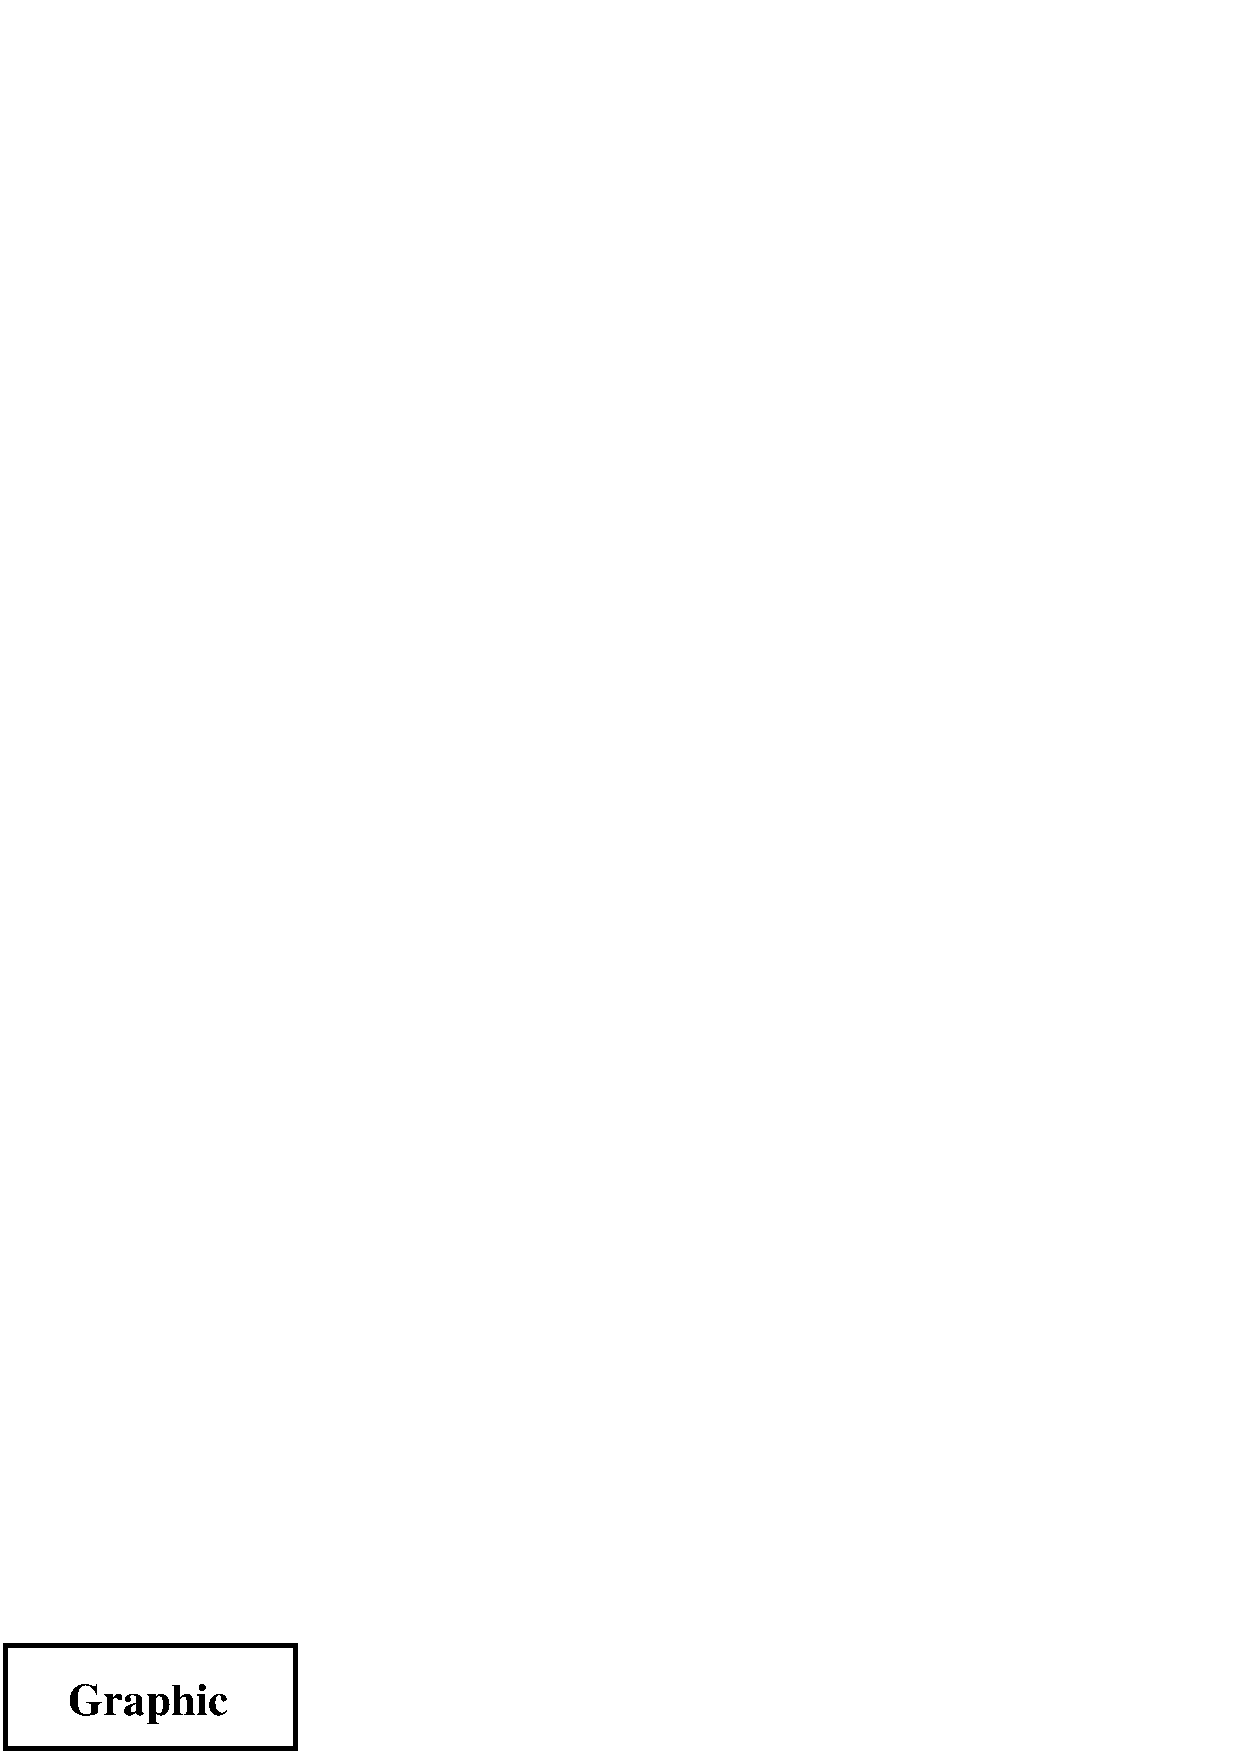
\includegraphics[width=1in]{graphic}% 
	\hspace{1in}% 
	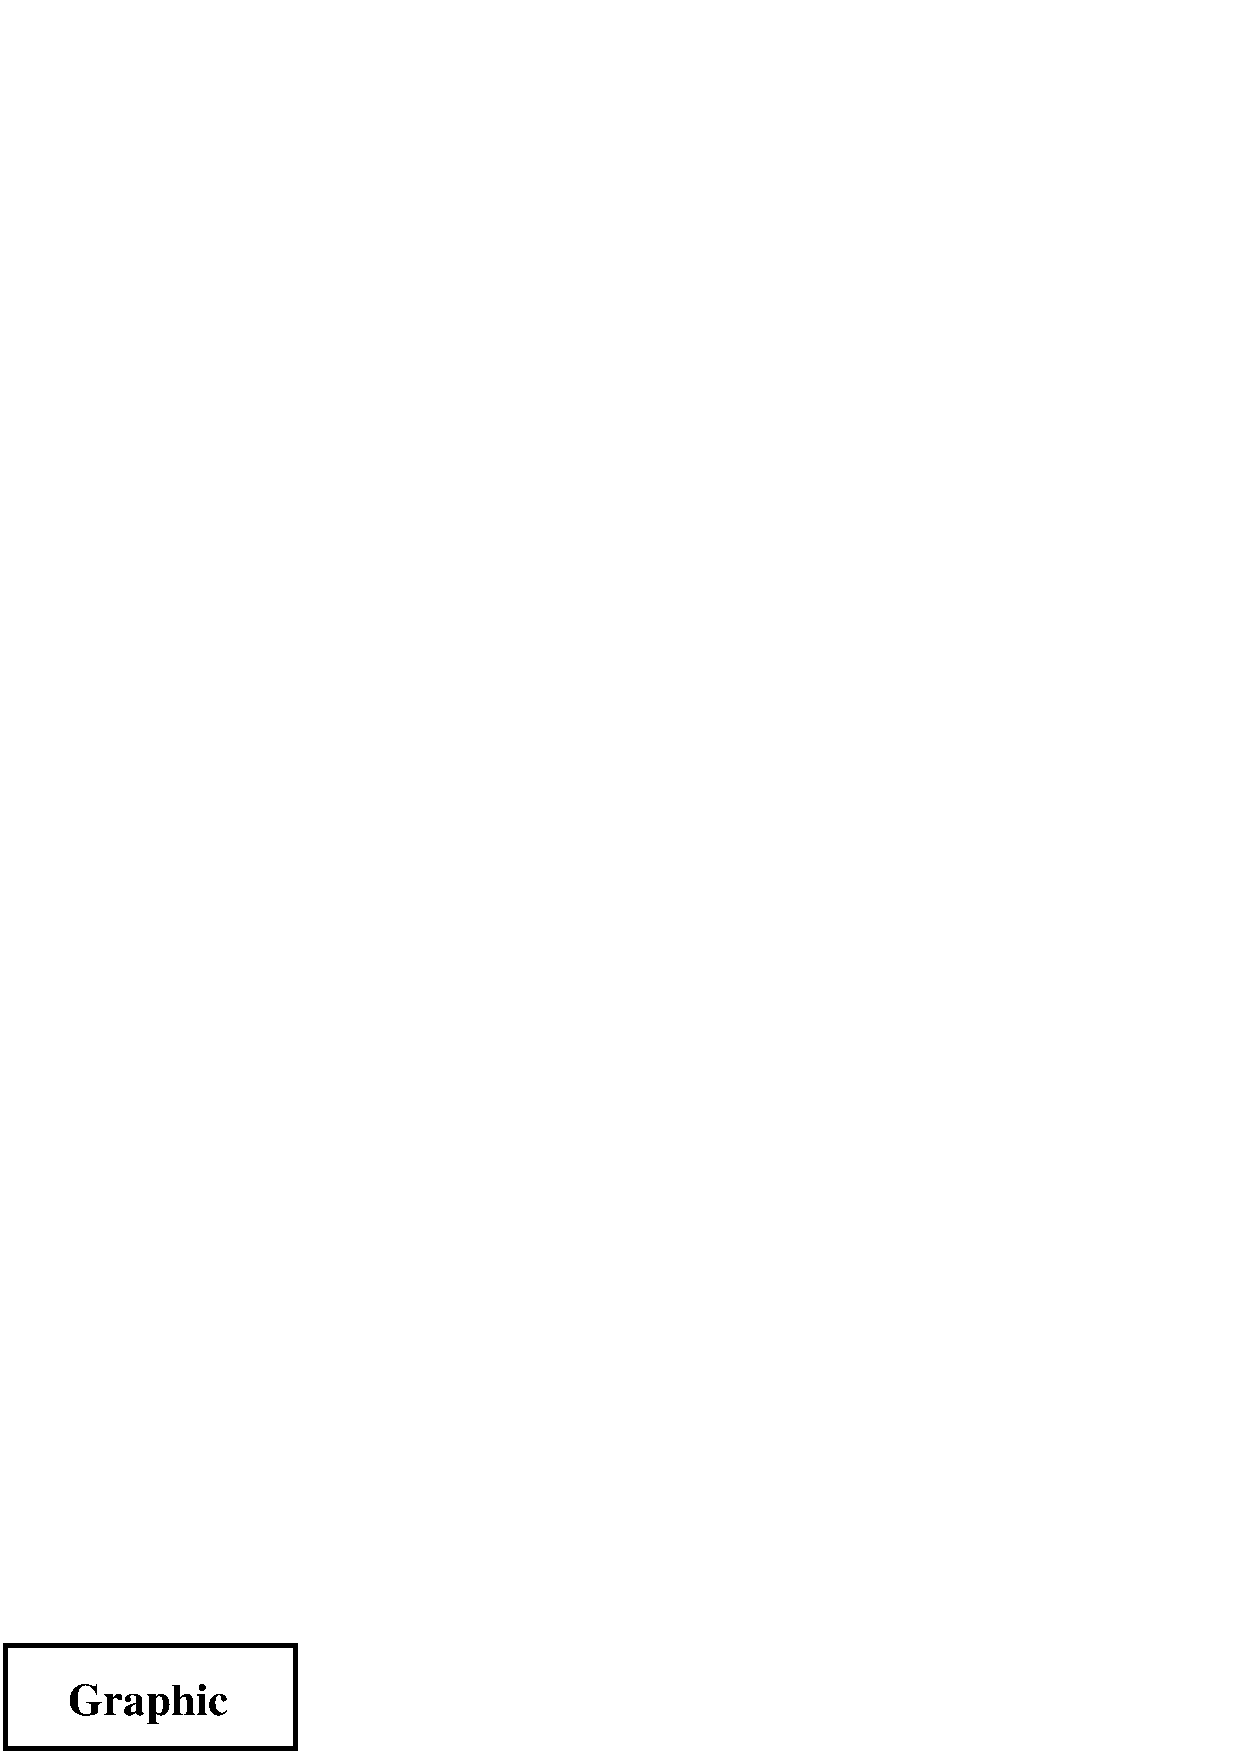
\includegraphics[width=2in]{graphic} 
	\caption{一个 figure 环境中的两幅图像} 
\end{figure}
\end{lstlisting}
会得到如图~\ref{fig:sidegraphics}~的并列图形。
该图形宽度为4英寸(第一幅图1英寸,\cmd{hspace}1英寸,第二幅图2英寸),居中放置。
其中的 \cmd{hspace} 命令可用 \cmd{hfill} 来代替,
这会将图形推向页面的两端边界(见第~\ref{ssec:hspace}~节)。

\begin{figure} 
	\centering 
	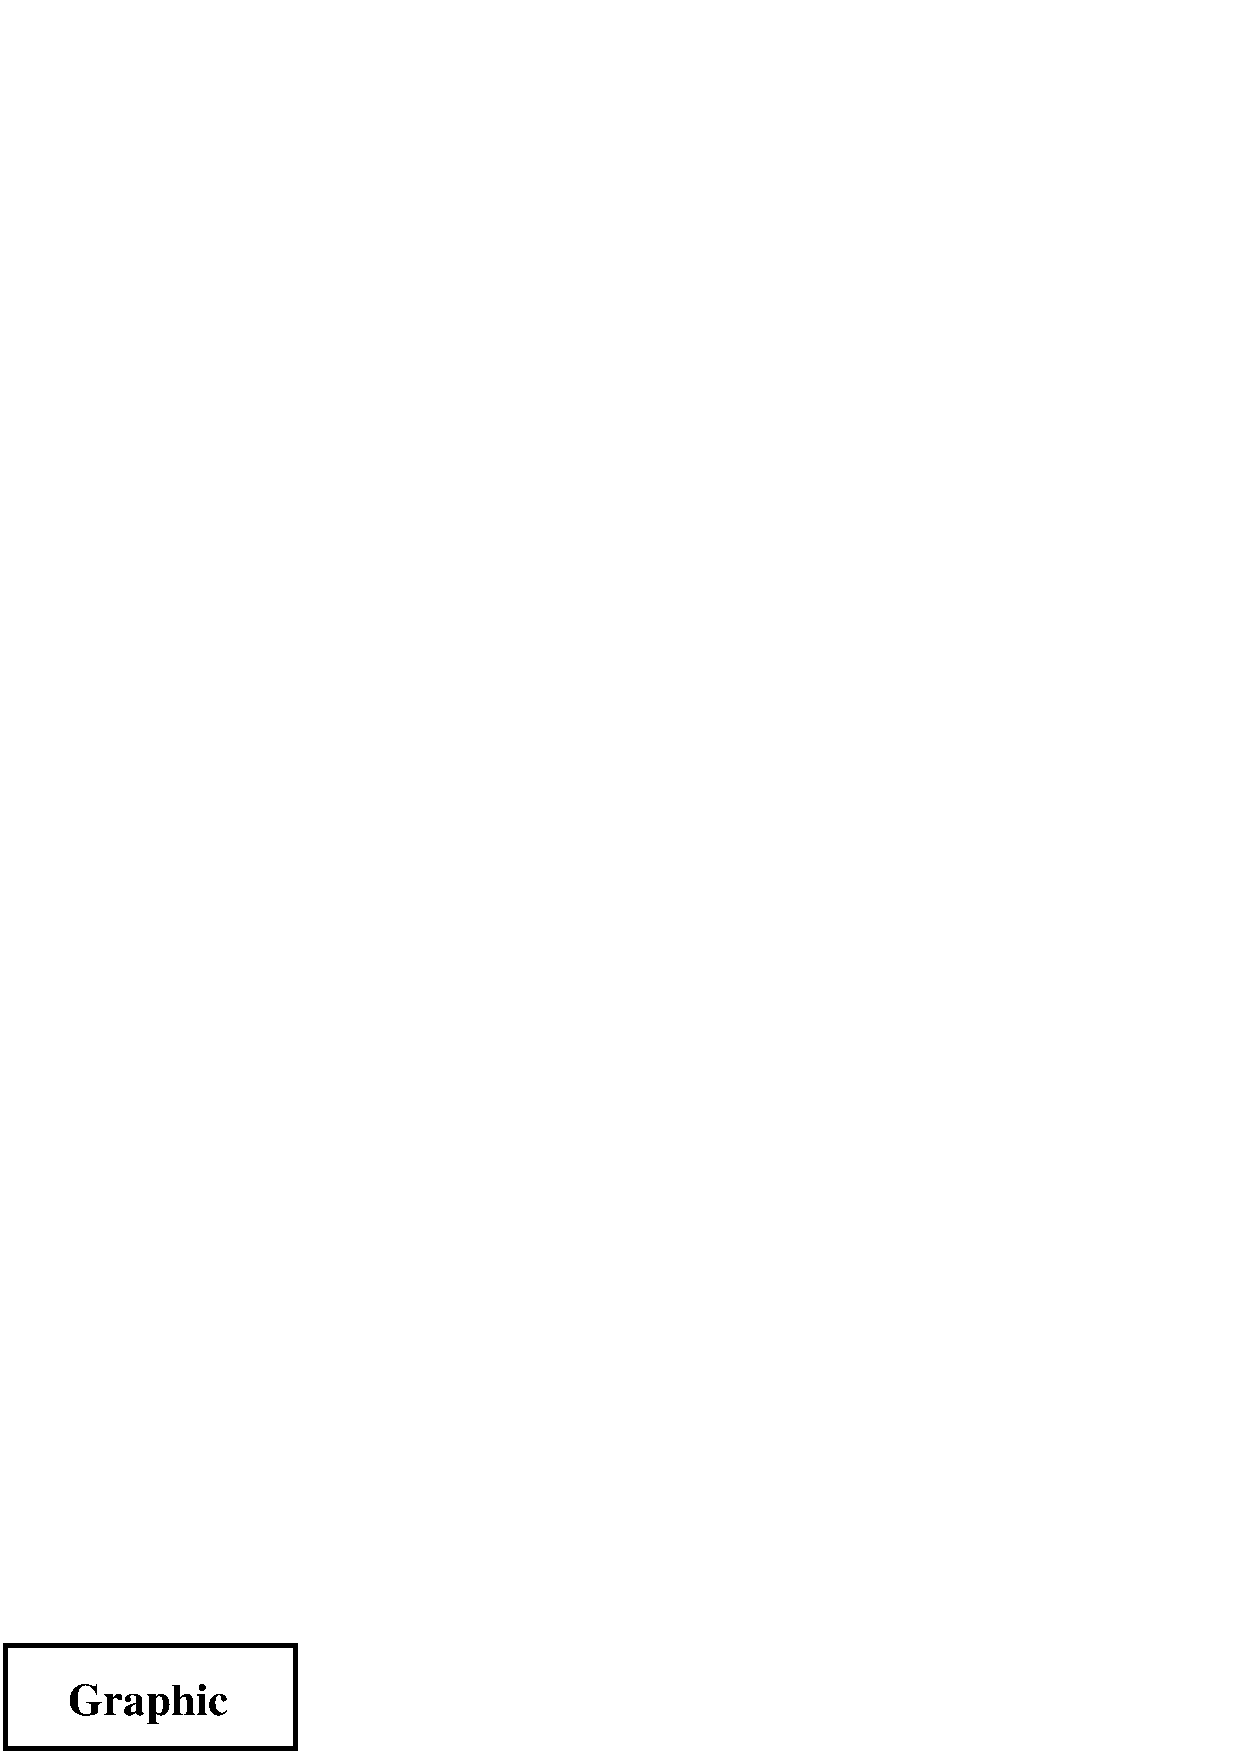
\includegraphics[width=1in]{graphic}% 
	\hspace{1in}% 
	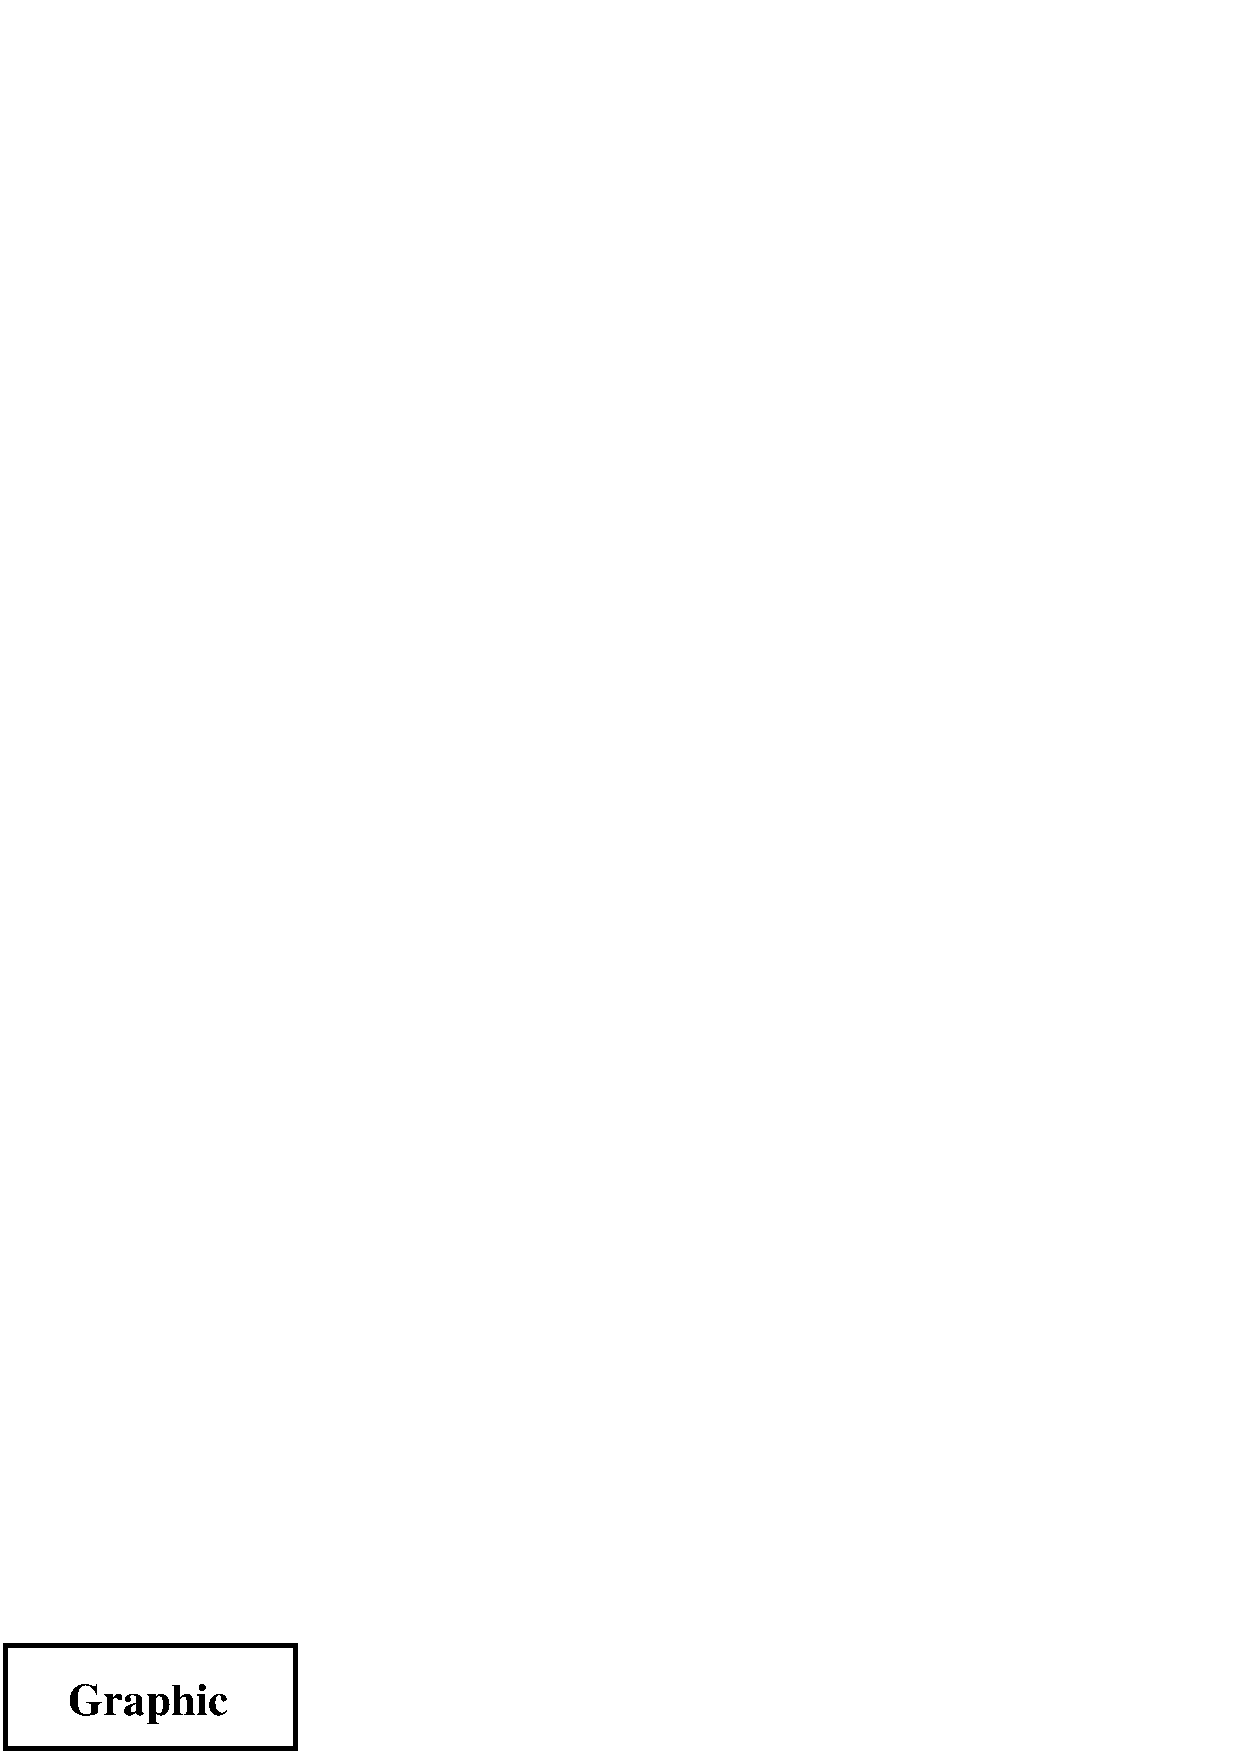
\includegraphics[width=2in]{graphic} 
	\caption{一个 \env{figure} 环境中的两幅图像}\label{fig:sidegraphics}
\end{figure}

\subsubsection{使用并列的小页环境}

Placing the \includegraphics commands inside minipage environments provides
the user more control over the graphics’ vertical placement. For example
\begin{figure}
	\centering
	\begin{minipage}[c]{0.5\linewidth}
		\centering 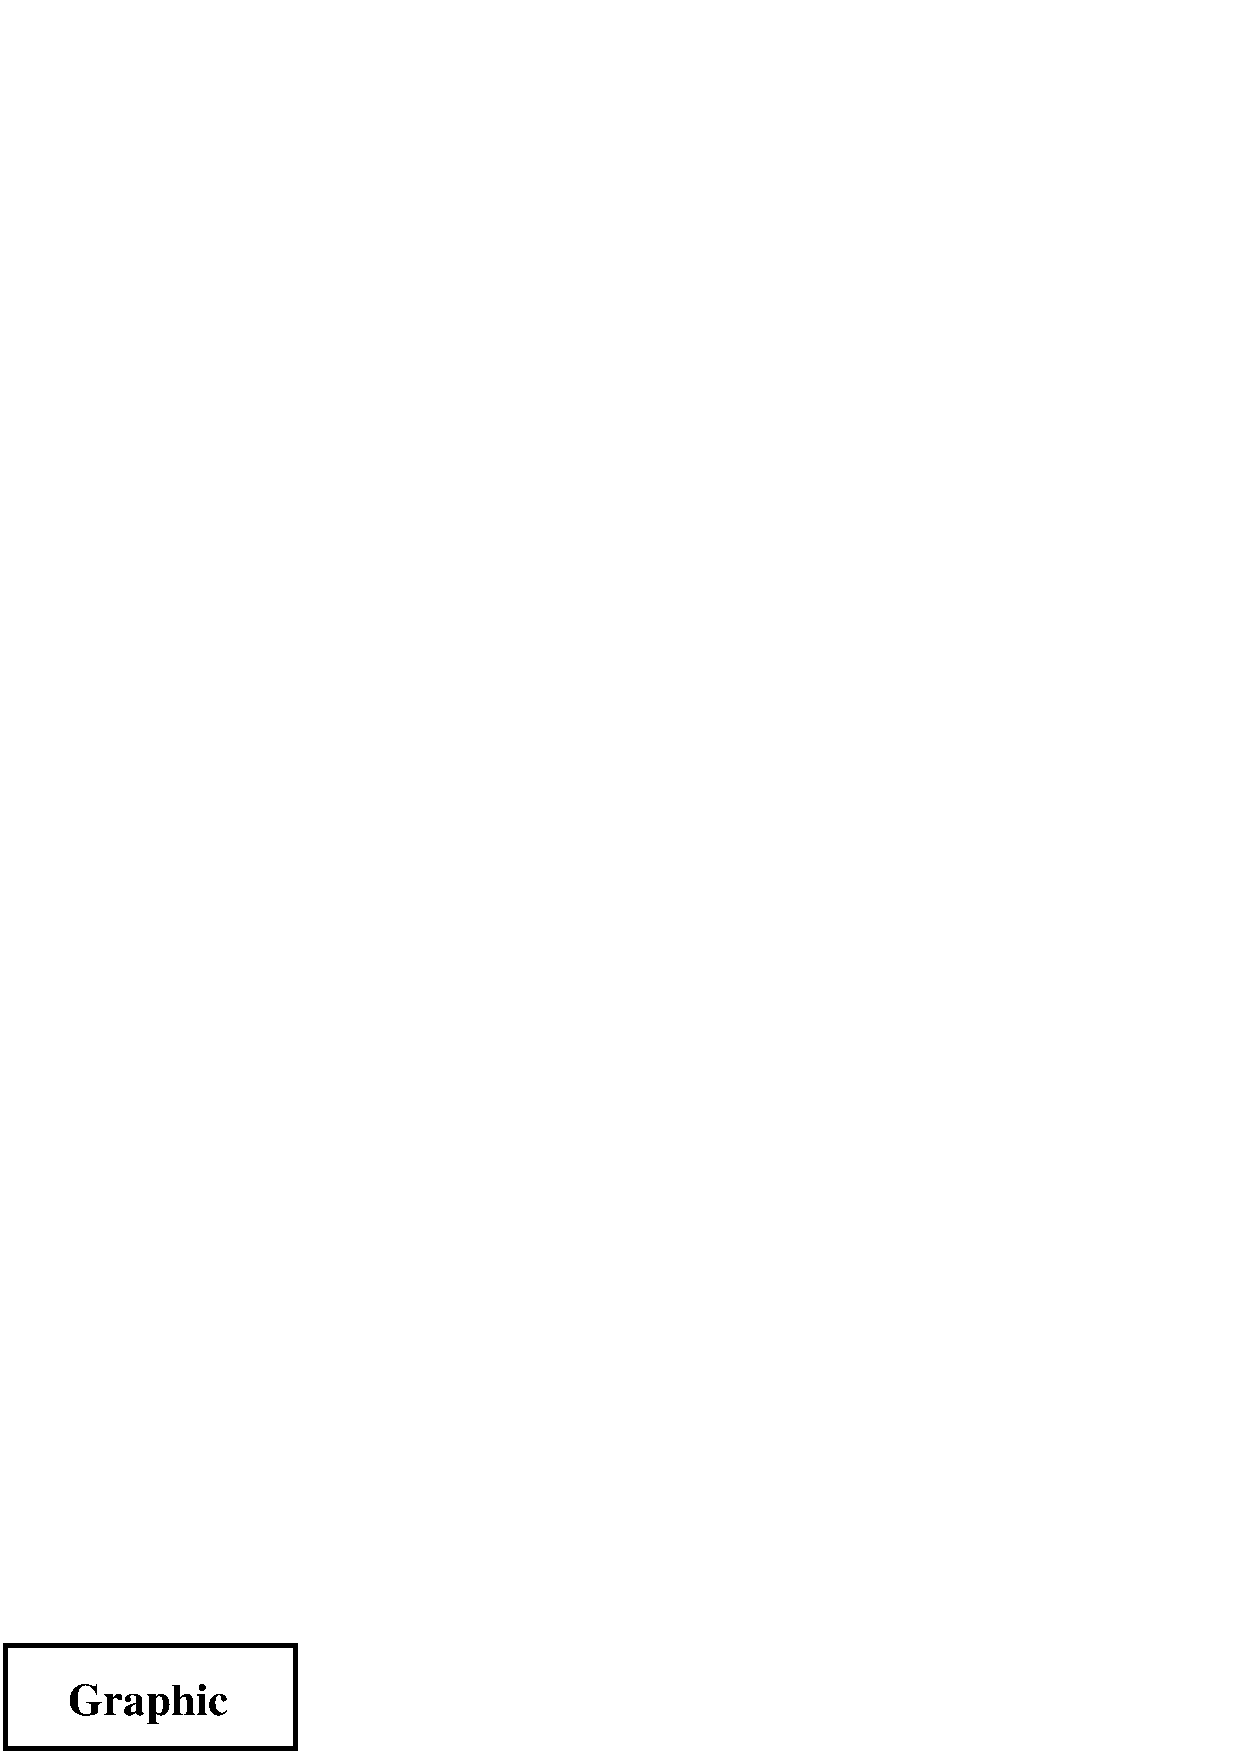
\includegraphics[width=1in]{graphic}
	\end{minipage}%
	\begin{minipage}[c]{0.5\linewidth}
		\centering 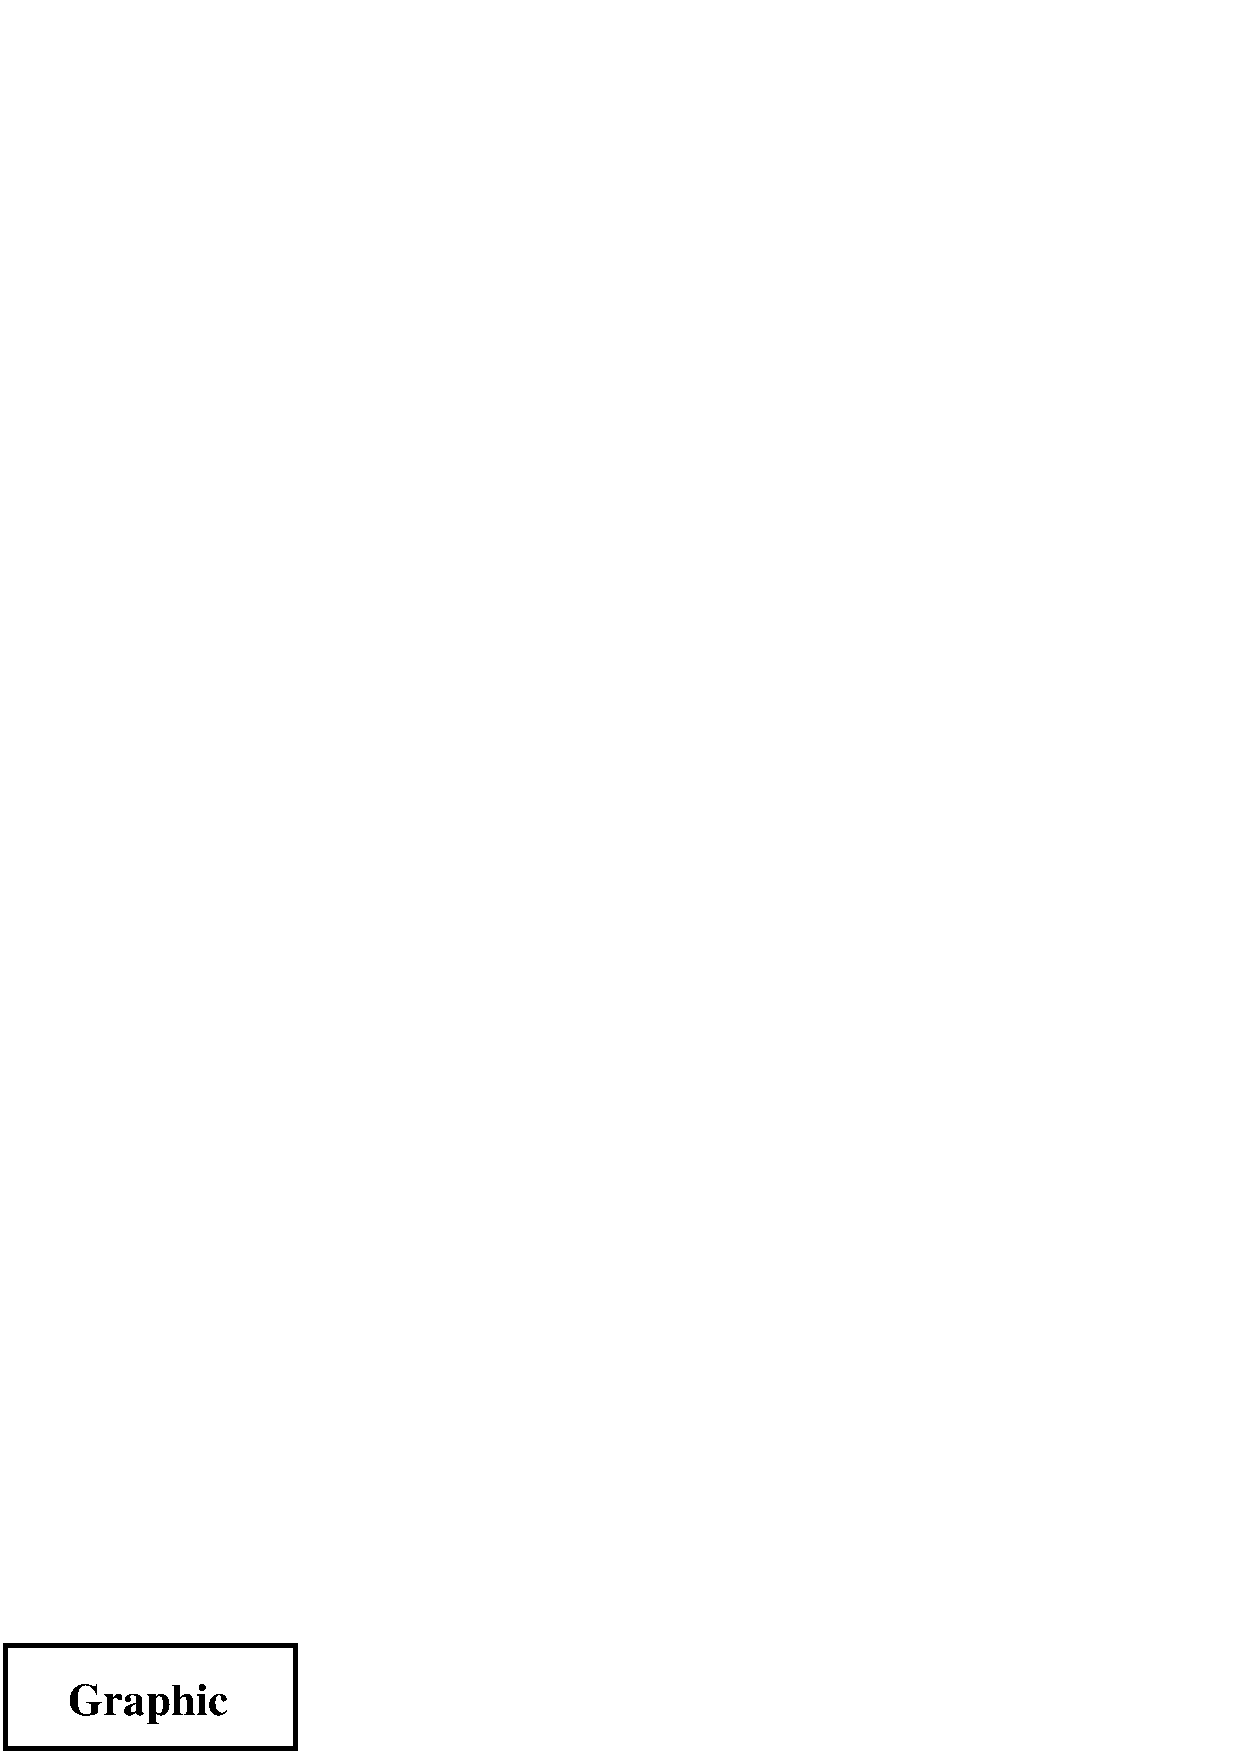
\includegraphics[width=2in]{graphic}
	\end{minipage}
	\caption{Centers Aligned Vertically}
\end{figure}
produces Figure 62, which has vertically-centered graphics.

将 \cmd{includegraphics} 命令放到小页环境中可以更好地控制图形的对齐方式。例如:
\begin{lstlisting}
\begin{figure} 
	\centering 
	\begin{minipage}[c]{0.5\textwidth} 
		\centering 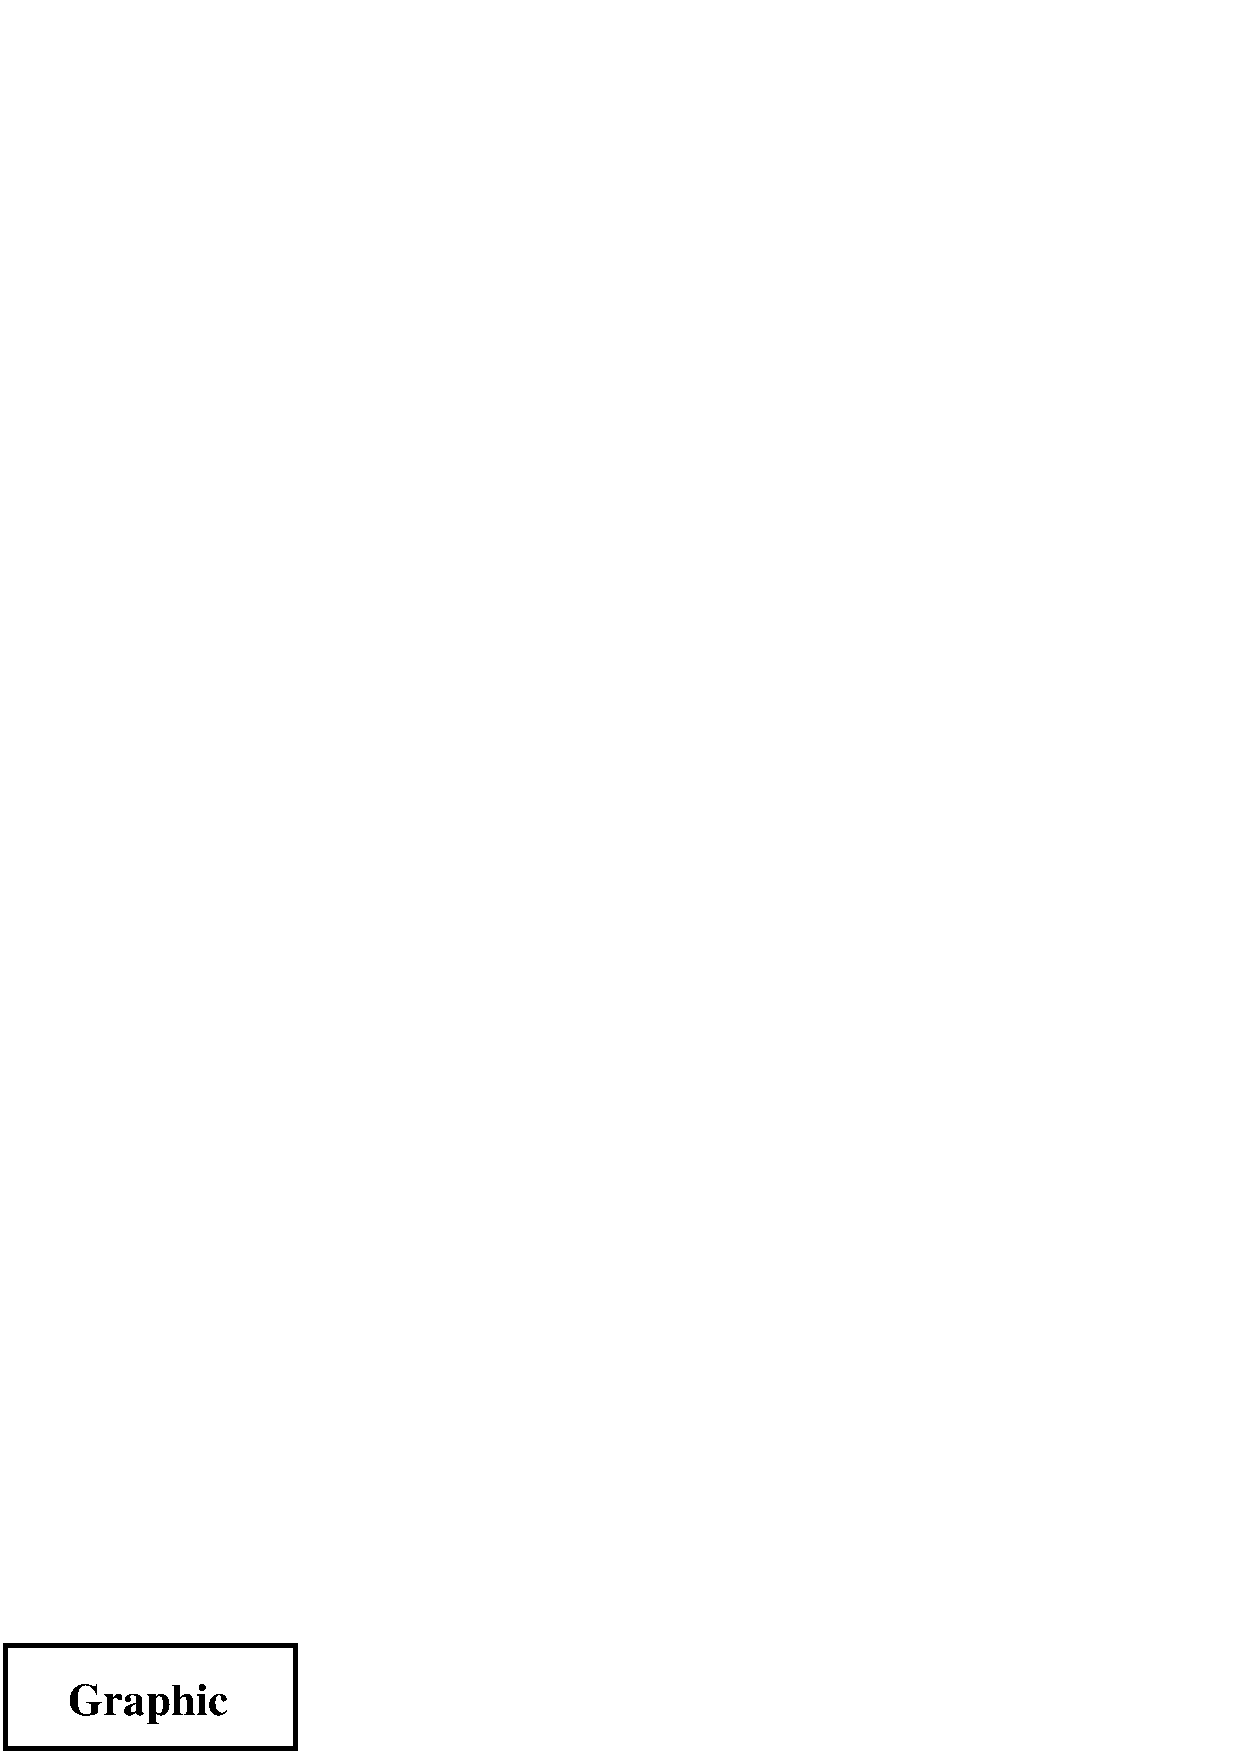
\includegraphics[width=1in]{graphic} 
	\end{minipage}% 
	\begin{minipage}[c]{0.5\textwidth} 
		\centering 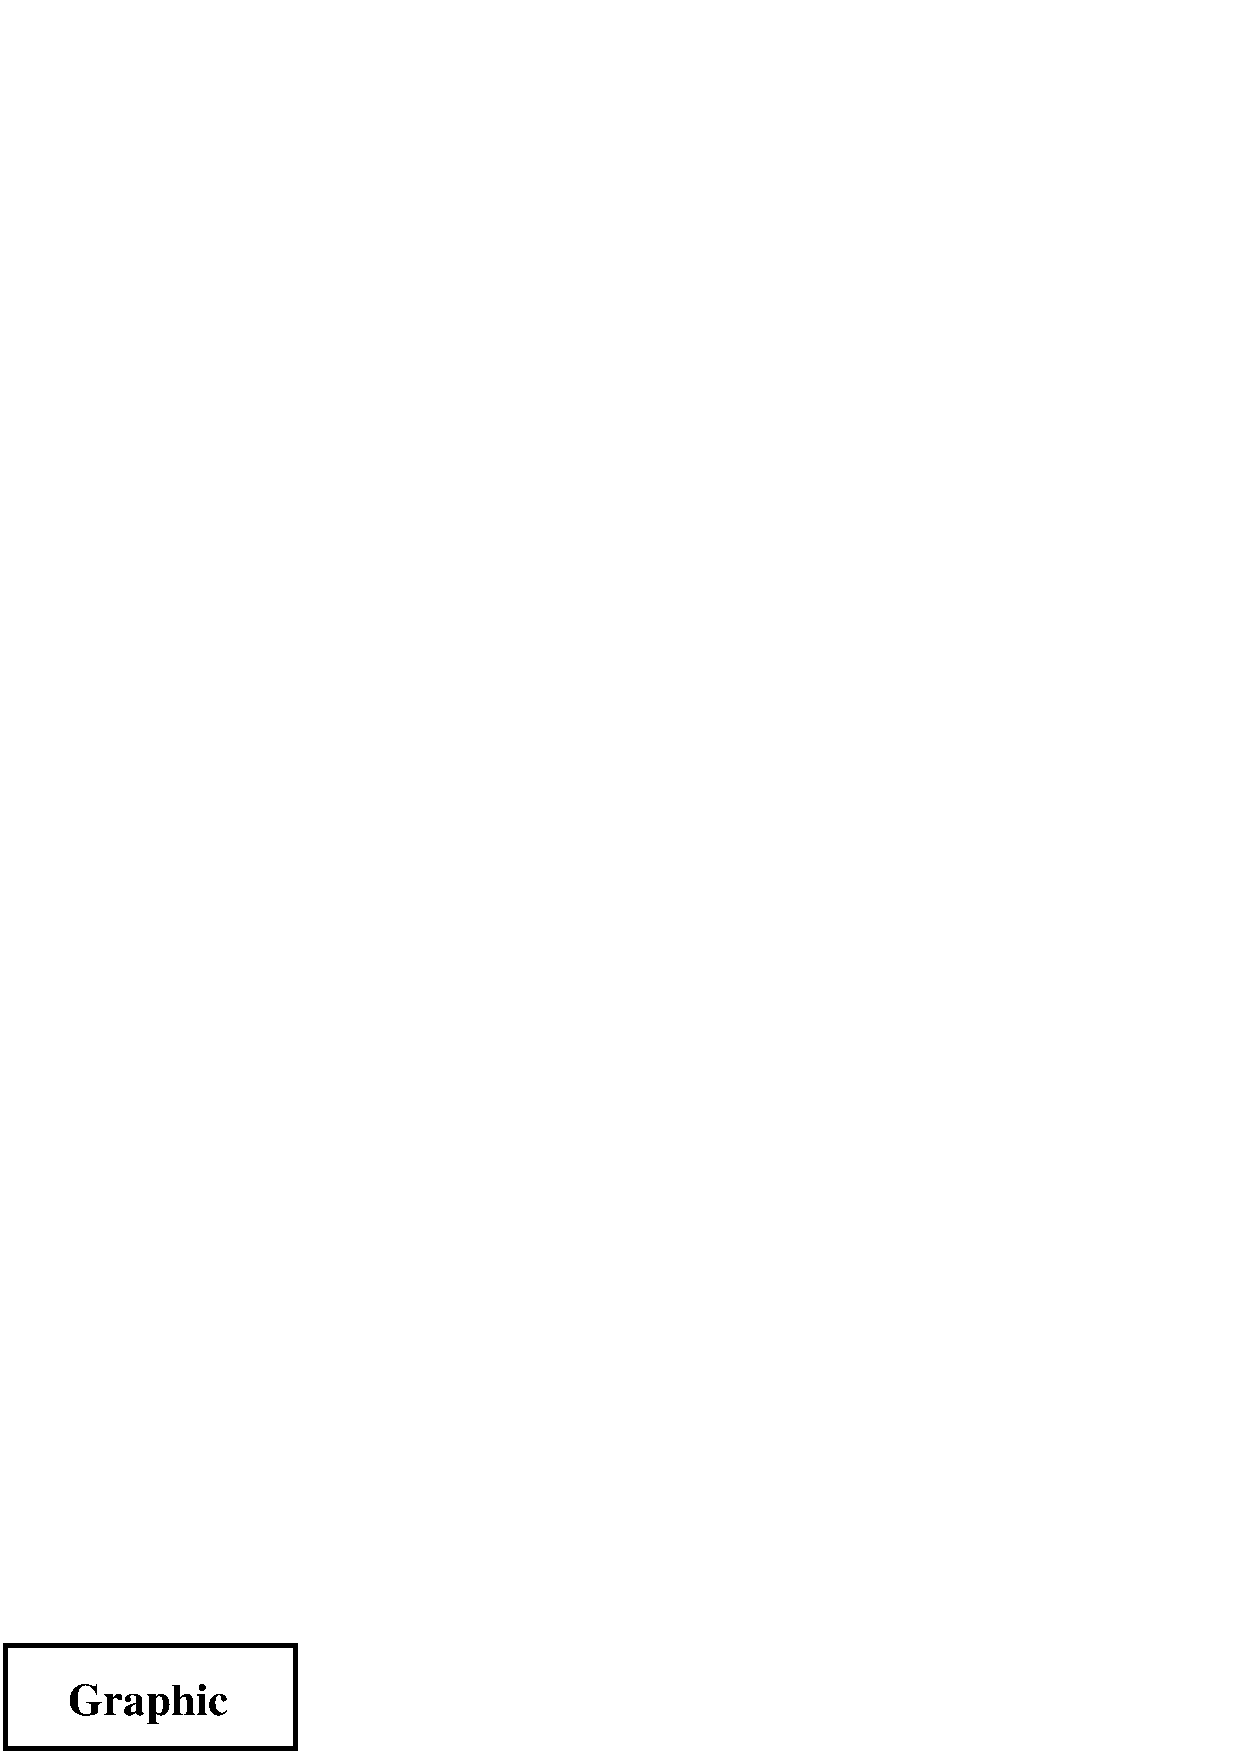
\includegraphics[width=2in]{graphic} 
	\end{minipage} 
	\caption{中间对齐的图像} 
\end{figure}
\end{lstlisting}
生成图~\ref{fig:minipagegraphics}~,其中的图形是中间对齐的。

\begin{figure} 
	\centering 
	\begin{minipage}[c]{0.5\textwidth} 
		\centering 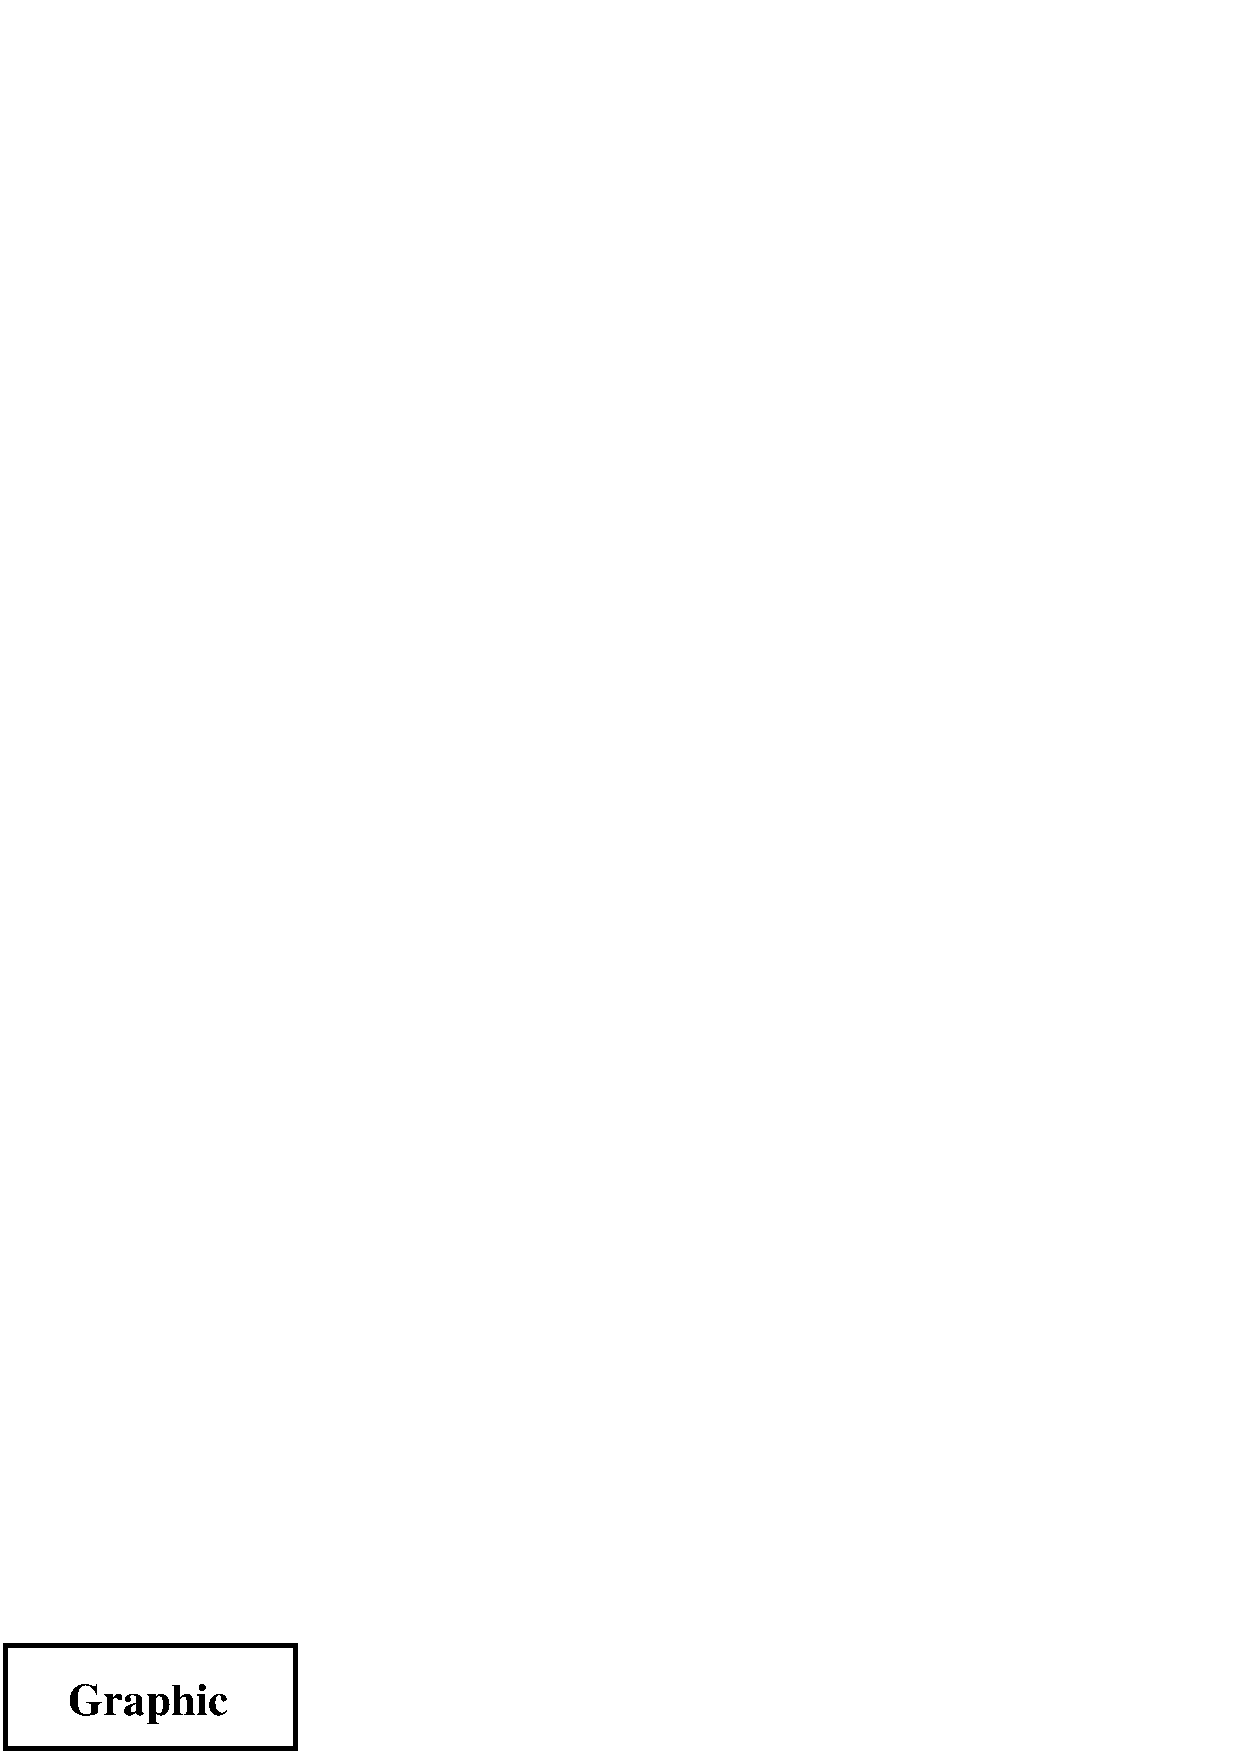
\includegraphics[width=1in]{graphic} 
	\end{minipage}% 
	\begin{minipage}[c]{0.5\textwidth} 
		\centering 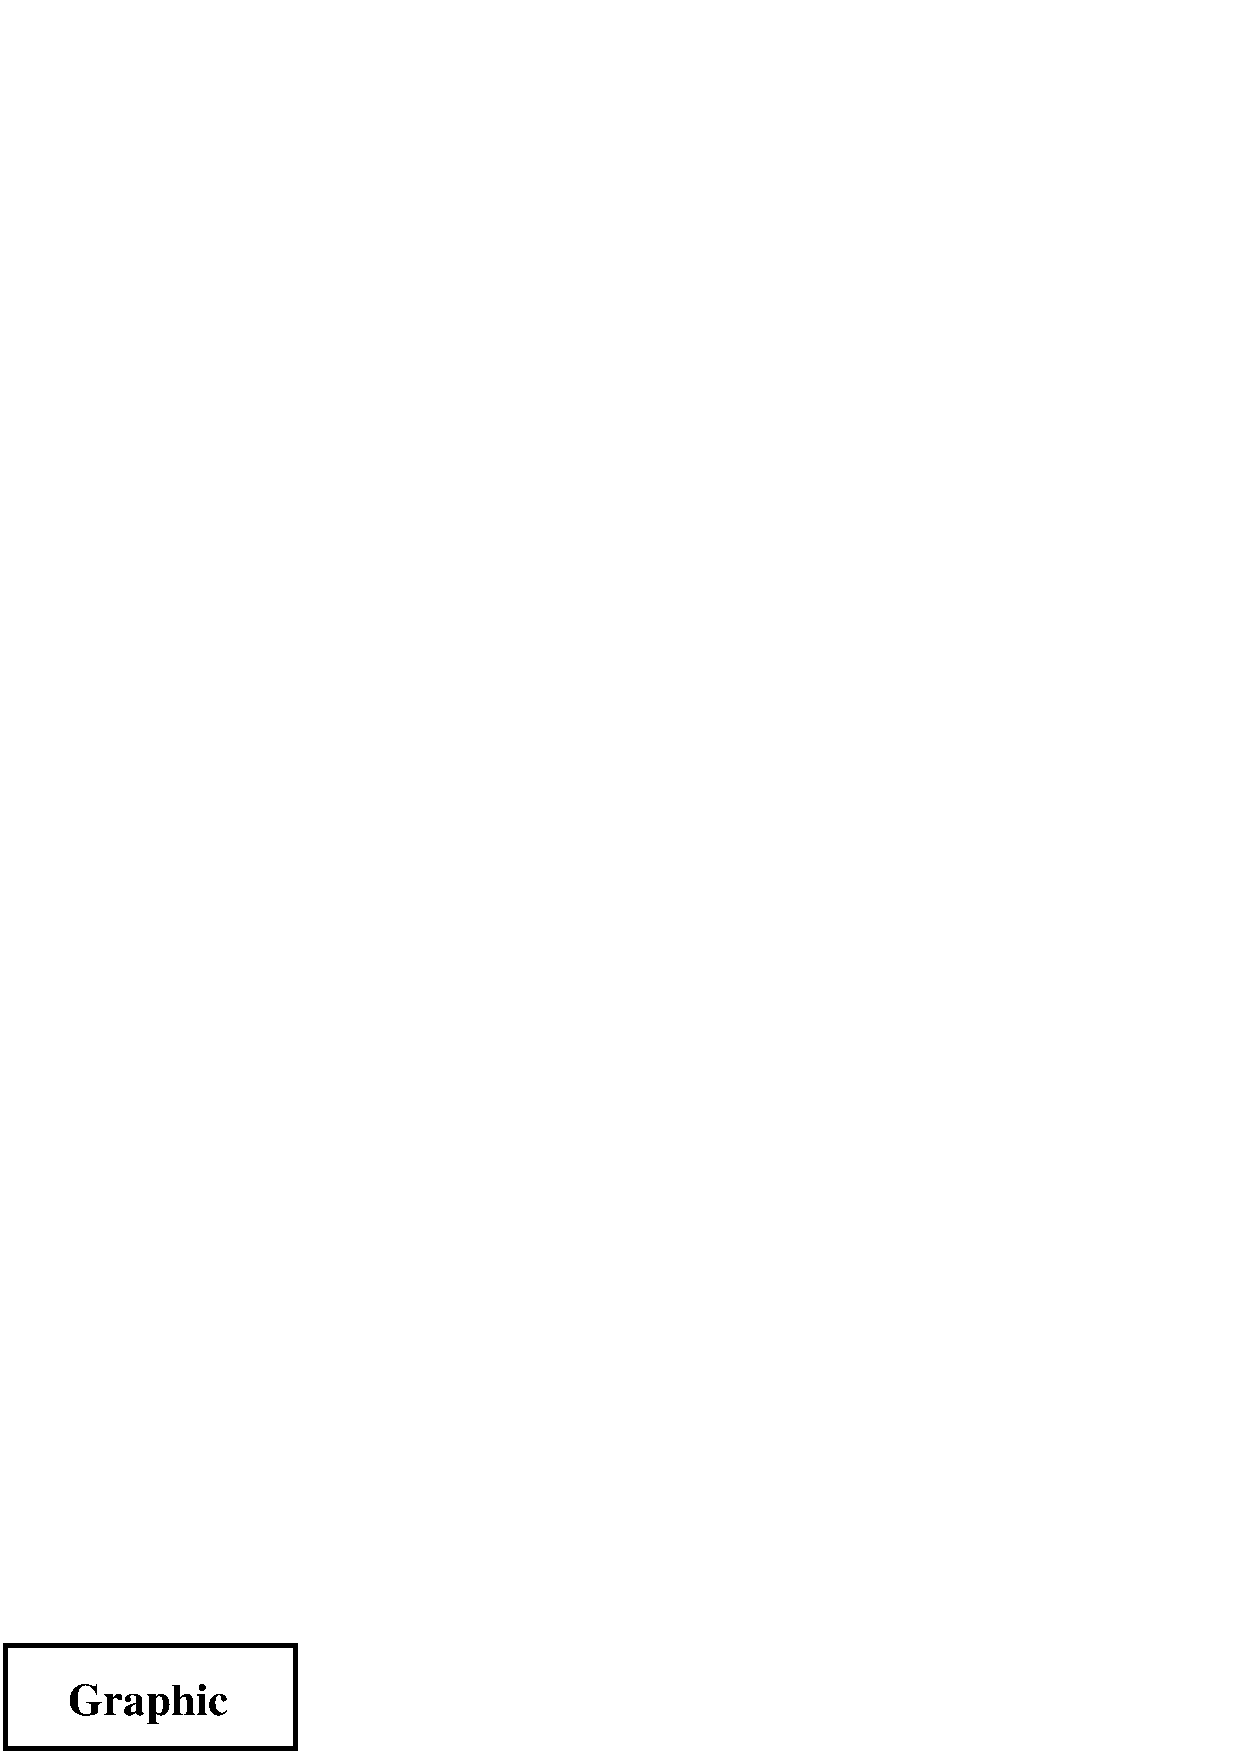
\includegraphics[width=2in]{graphic} 
	\end{minipage} 
	\caption{中间对齐的图像} \label{fig:minipagegraphics}
\end{figure}

对于这个例子,需要注意以下几点:
\begin{itemize}
	\item 如同其它的 \LaTeX{} 对象一样,小页在放置时,它的参考点和当前基线对齐。
	缺省情况下小页使用 \opt{[c]} 选项,将参考点置于其竖直方向的中点。
	选项 \opt{[t]} 将参考点置于小页顶行的基线上,
	而选项 \opt{[b]} 将参考点置于小页底行的基线上(参见第~\ref{ssec:minivalign}~节)。
	
	\item 在第一个 \cmdonearg{end}{minipage} 后面的 \texttt{\%} 防止在两个小页之间多一个空格
	(参见第~\ref{ssec:hspace} 节)。
	
	\item 当几个并列小页的宽度之和没有达到 $1.0\text{\cmd{textwidth}}$ 时,
	可用 \cmd{hspace} 或 \cmd{hfill} 来确定水平间距,详见第~\ref{ssec:hspace}~节。
\end{itemize}


\subsection{并列的浮动图形}\label{ssec:sidefigure}

在上一节中,通过在一个图形环境中使用多个小页环境得到一个由多幅图像组成的浮动图形。
若将  \cmd{caption} 命令放到每个小页环境中,则每个小页环境自己就变成浮动图形。例如:
\begin{lstlisting}
\begin{figure}
	\centering
	%%----start of first figure----
	\begin{minipage}[t]{0.4\linewidth}
		\centering
		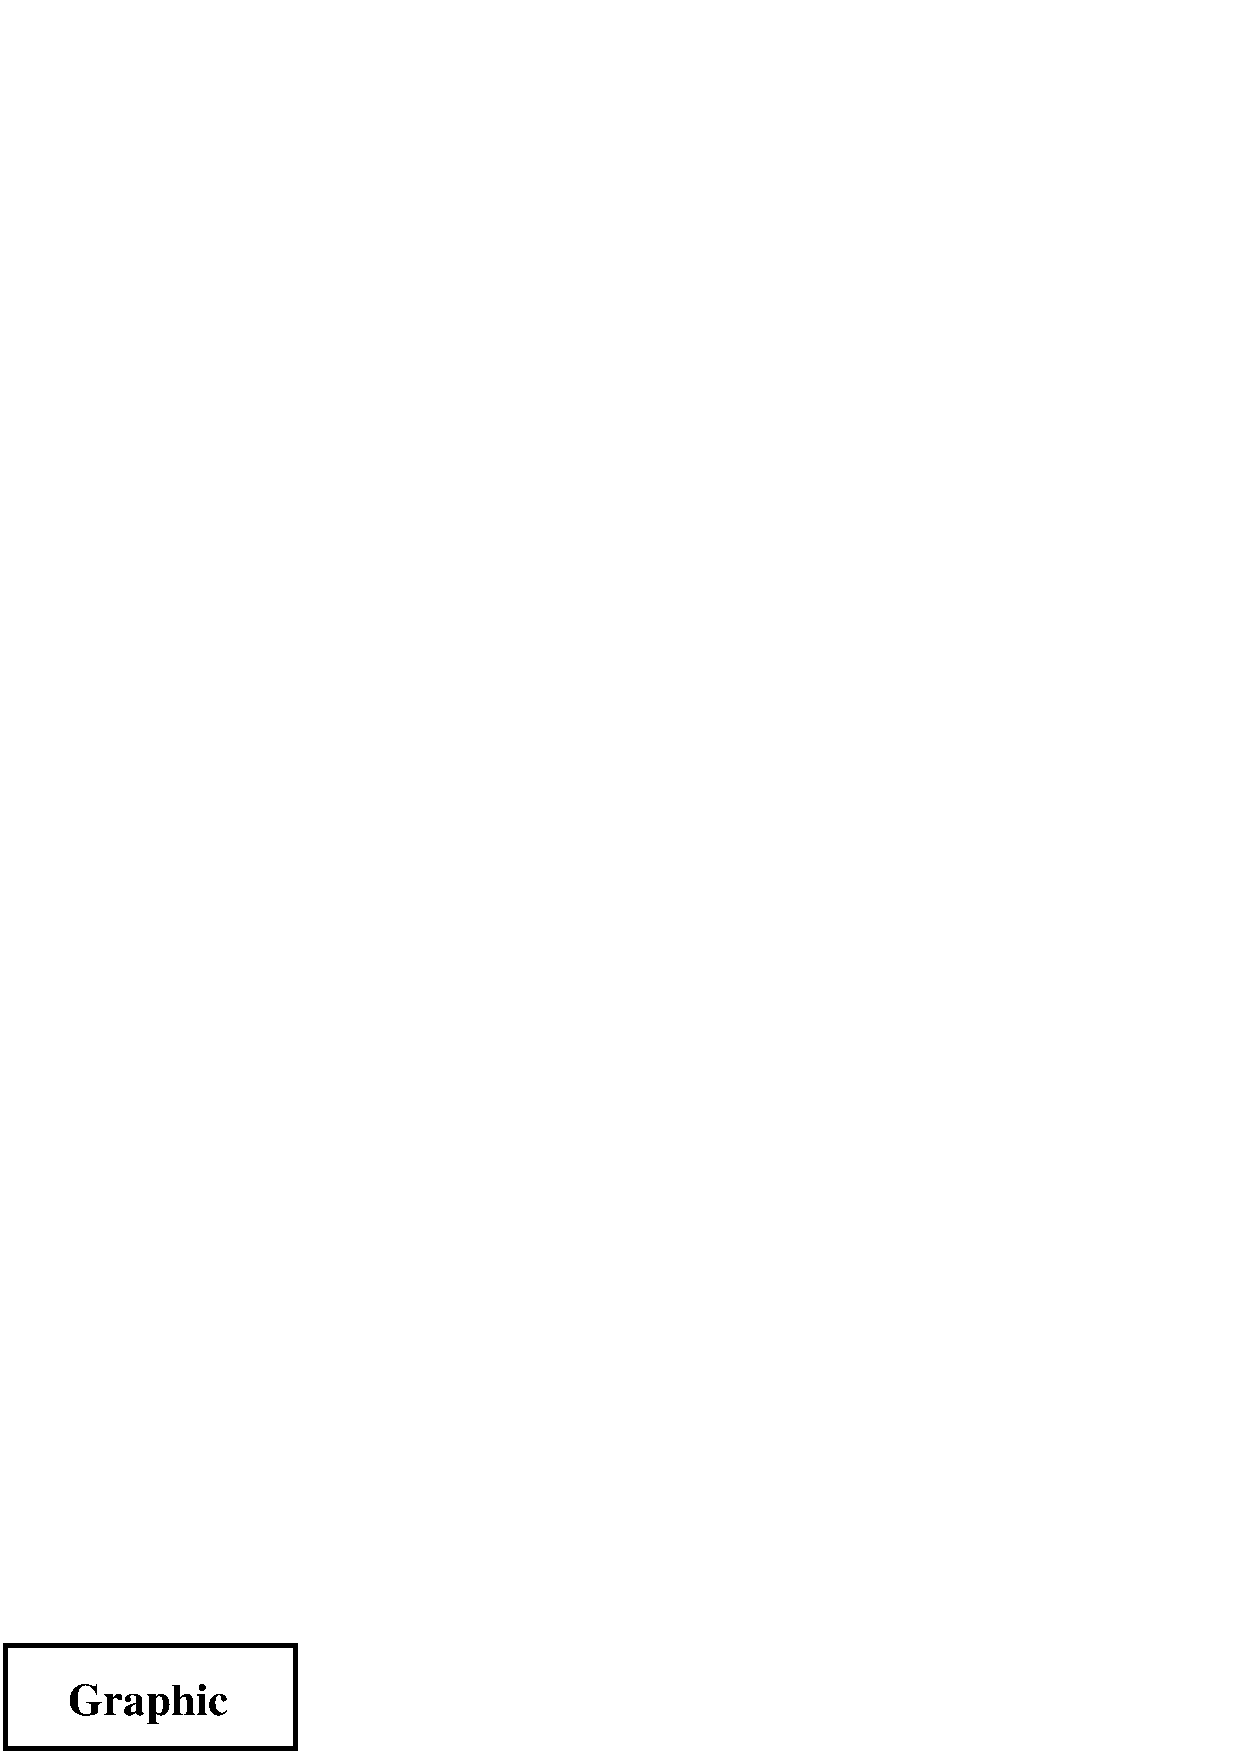
\includegraphics[width=1in]{graphic}
		\caption{Small Box} \label{fig:side:a}
	\end{minipage}%
	\hspace{1cm}%
	%%----start of second figure----
	\begin{minipage}[t]{0.4\linewidth}
		\centering
		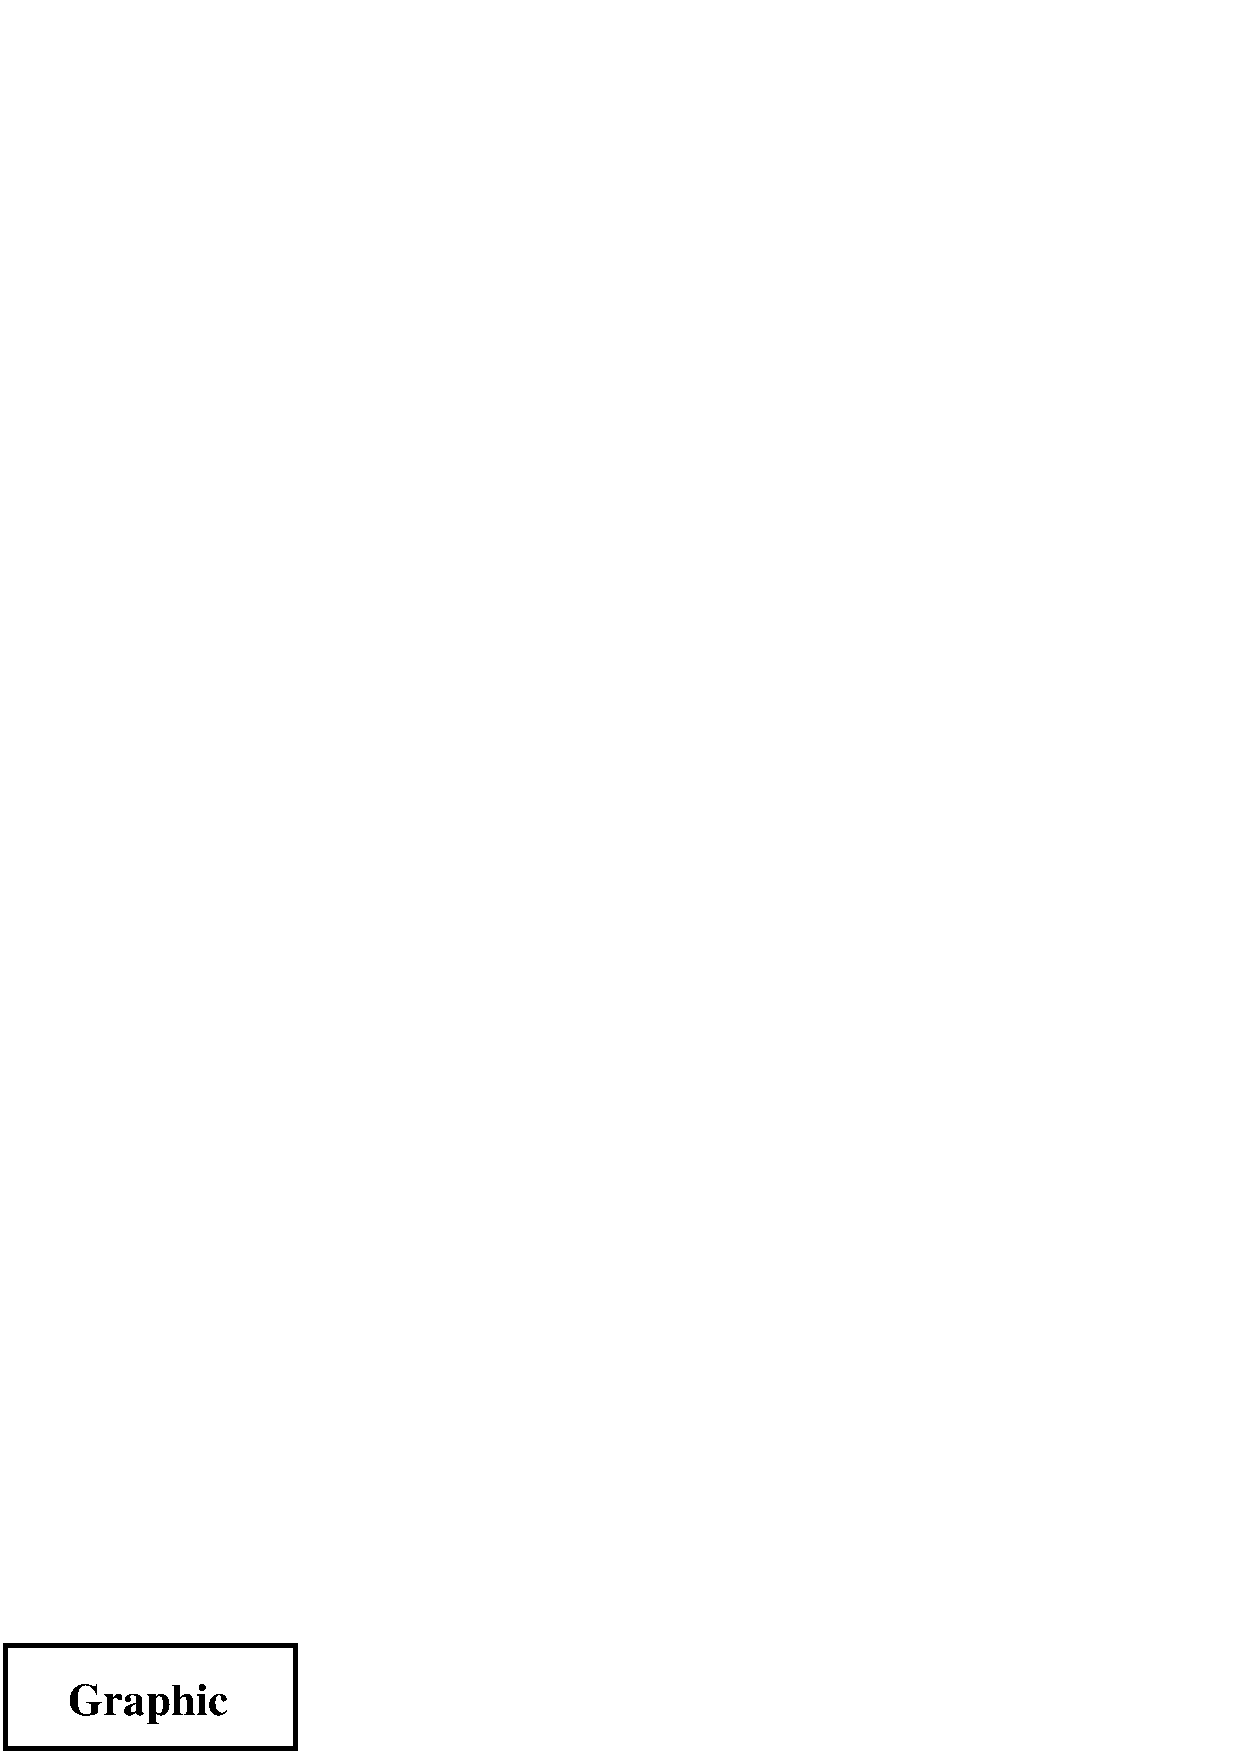
\includegraphics[width=1.5in]{graphic}
		\caption{Big Box} \label{fig:side:b}
	\end{minipage}
\end{figure}
\end{lstlisting}
生成图~\ref{fig:side:a}~和~\ref{fig:side:b}。

\begin{figure}
	\centering
	%%----start of first figure----
	\begin{minipage}[t]{0.4\linewidth}
		\centering
		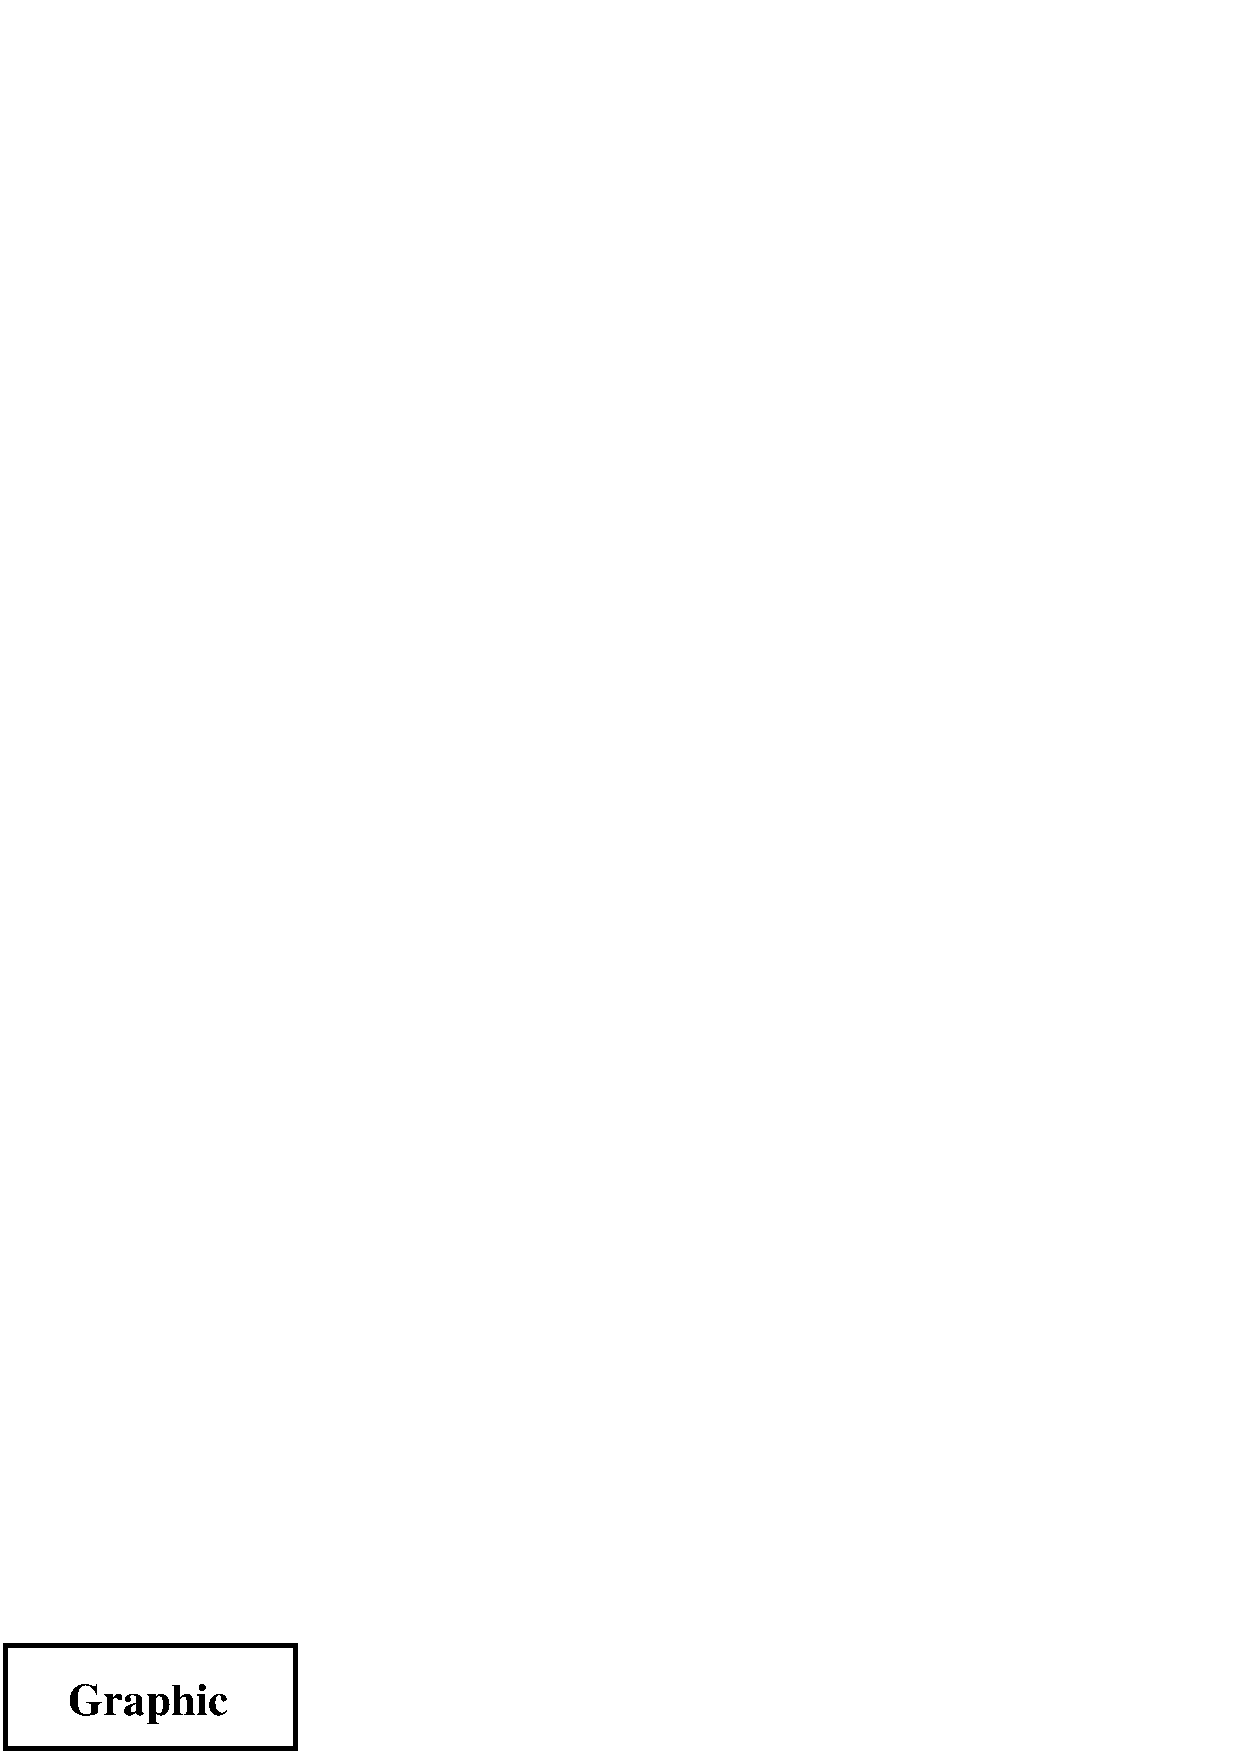
\includegraphics[width=1in]{graphic}
		\caption{Small Box} \label{fig:side:a}
	\end{minipage}%
	\hspace{1cm}%
	%%----start of second figure----
	\begin{minipage}[t]{0.4\linewidth}
		\centering
		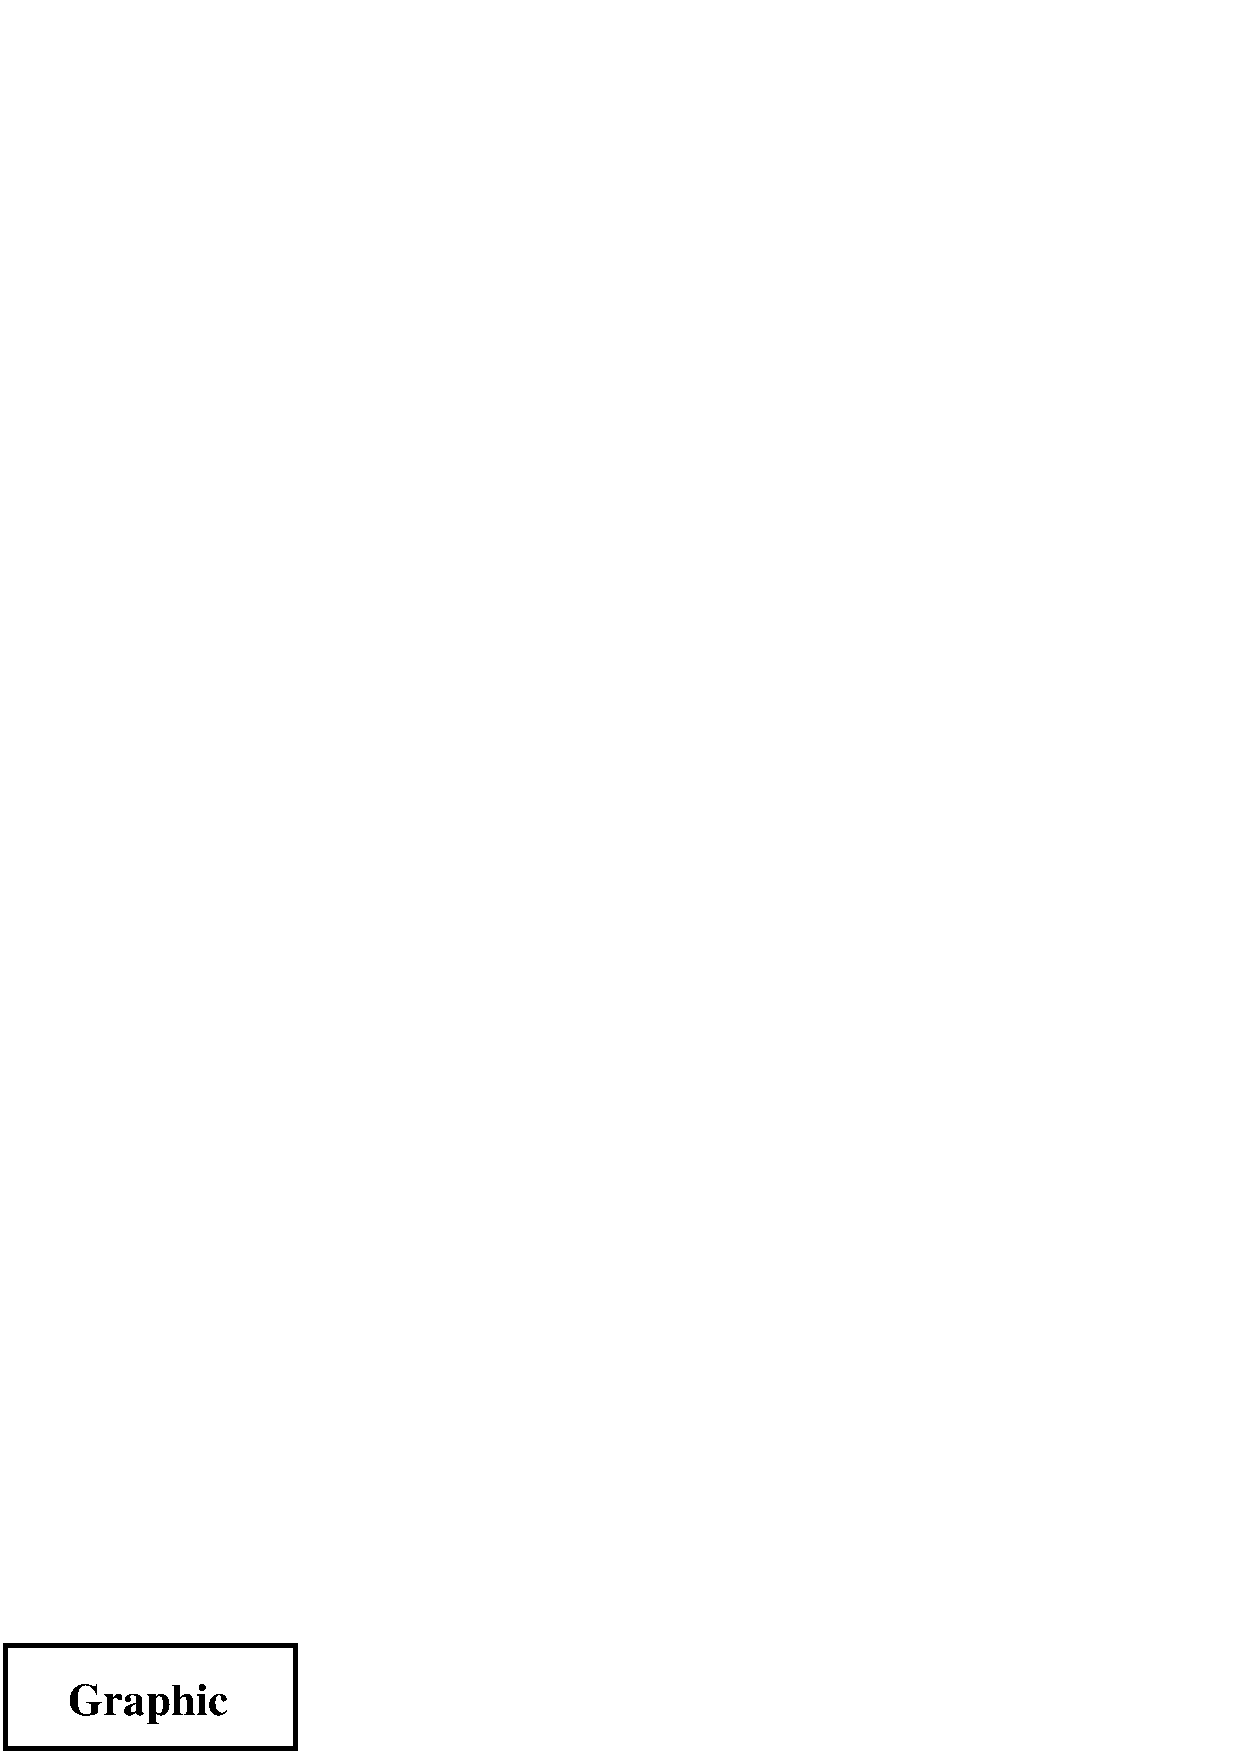
\includegraphics[width=1.5in]{graphic}
		\caption{Big Box} \label{fig:side:b}
	\end{minipage}
\end{figure}

关于该例子有几个注记:
\begin{itemize}
	\item 尽管上面的命令只使用了一个 \env{figure} 环境,
	但由于每个小页中都包含 \cmd{caption} 命令,所以仍然得到两个浮动图形。
	
	\item 两个放置图像的小页环境宽度为 \env{figure} 环境宽度的 $40\percent$,
	之间有1厘米的水平间距。
	(注意,在 \cmdonearg{end}{minipage} 和 \cmdonearg{hspace}{1cm} 之后的注释会阻止额外的空格,
	从而确保了间距正好是1厘米。)
	
	默认情况下,图形标题的宽度就是小页环境的宽度。
	使用1厘米的水平间距是为了确保标题之间有空白(无论对长标题还是很宽的图像)。
	
	此外,标题的宽度也可以用 \pkg{caption} 宏包的 \opt{margin} 或 \opt{width} 关键字进行控制
	(参见表~\ref{tab:caption-formatopt})。
	
	\item 紧接着 \cmdonearg{begin{figure} 的 \cmd{centering} 命令使得两个小页以及之间的空白在 \env{figure} 环境中居中放置。
		
	\item 小页内部的 \cmd{centering} 命令使得图像在小页环境内部居中放置。
\end{itemize}

\subsection{并列的子图形}\label{ssec:sidesubfigure}

在某些情况下,有时会希望将并列的图形组成一组,同时其中的每一幅图都保持其独立性。
\pkgi{subfig} 宏包的 \cmdi{subfloat} 命令(参见第~\ref{sec:subfig-pkg} 节)
可以将一组独立的图像作为一个 \env{figure} 环境中的子图。
例如:
\begin{lstlisting}
\usepackage{subfig}
...
\begin{figure}
	\centering
	%%----start of first subfigure----
	\subfloat[Small Box with a Long Caption]{
		\label{fig:subfig:a} %% label for first subfigure
		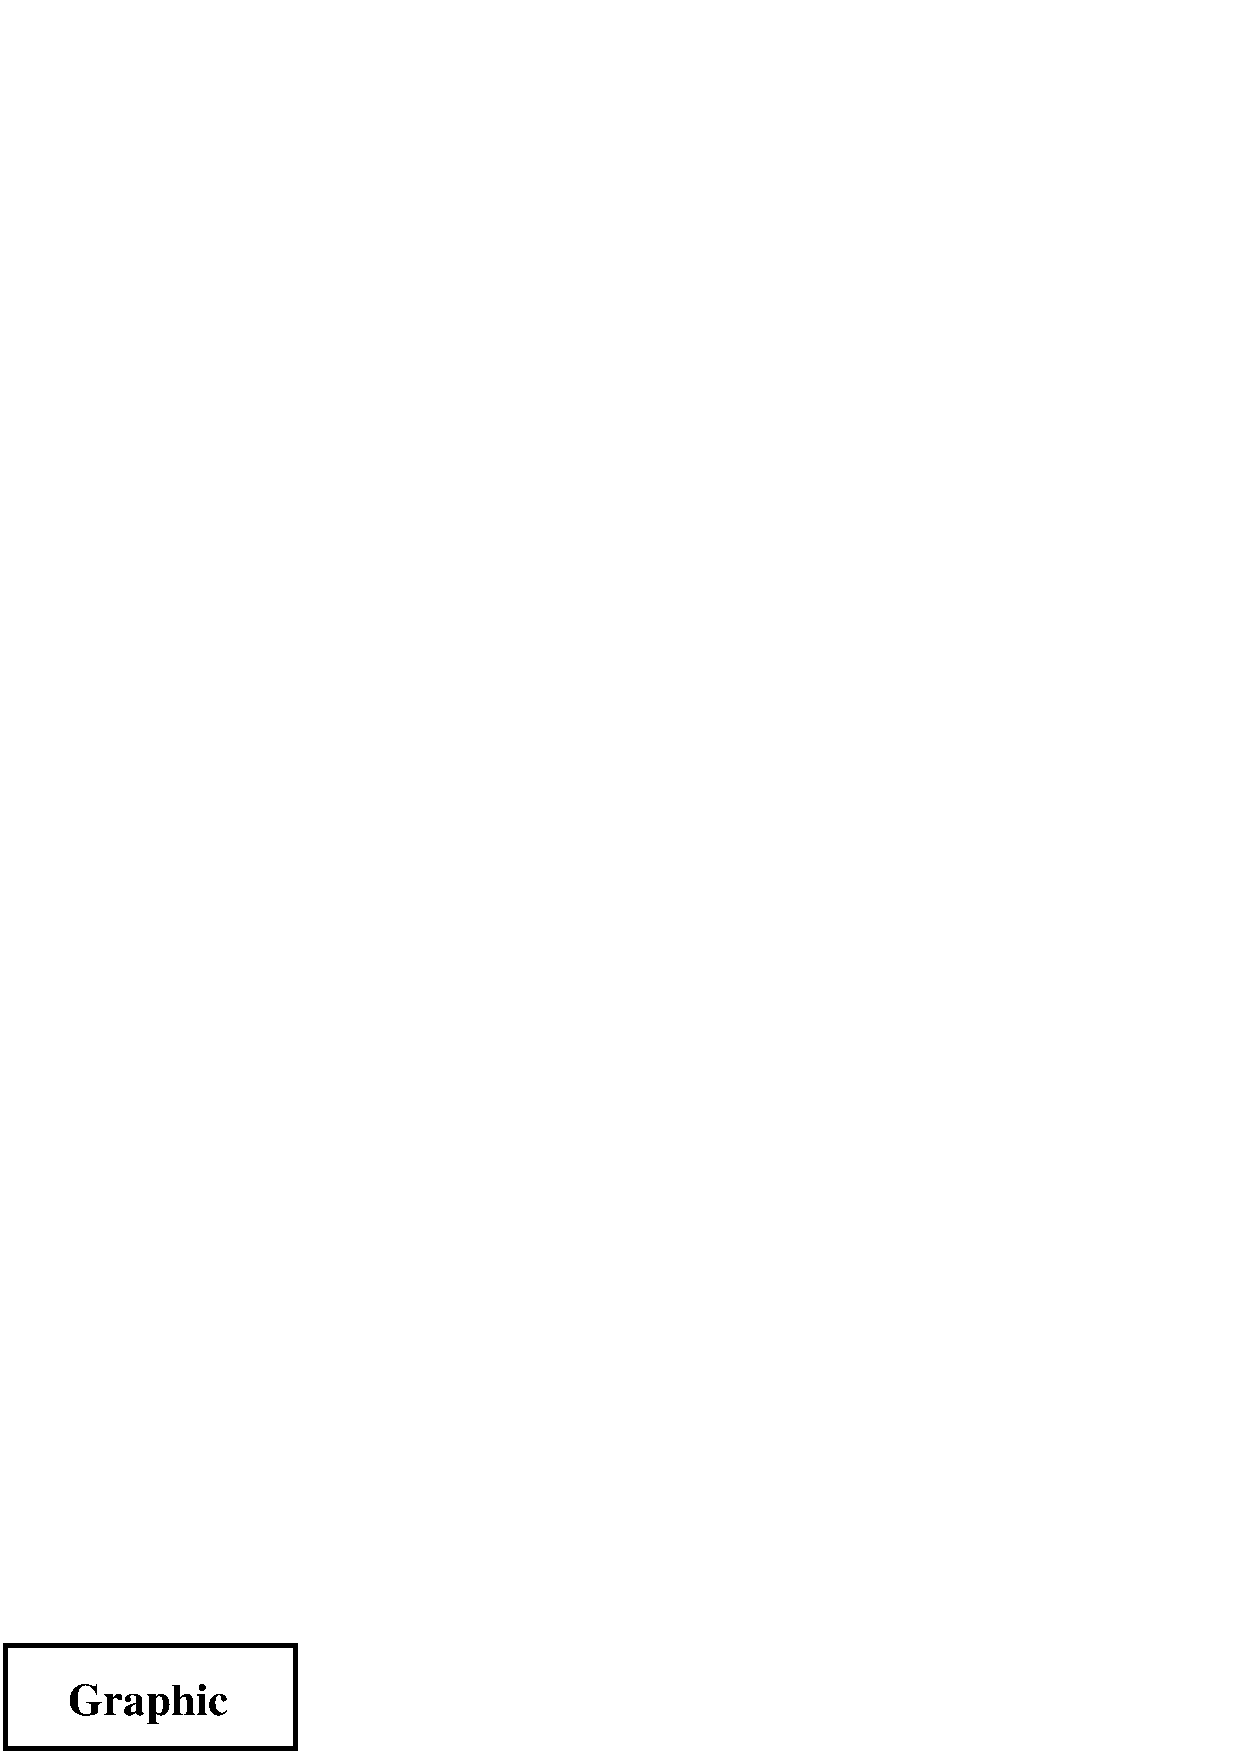
\includegraphics[width=1.0in]{graphic}}
	\hspace{1in}
	%%----start of second subfigure----
	\subfloat[Big Box]{
		\label{fig:subfig:b} %% label for second subfigure
		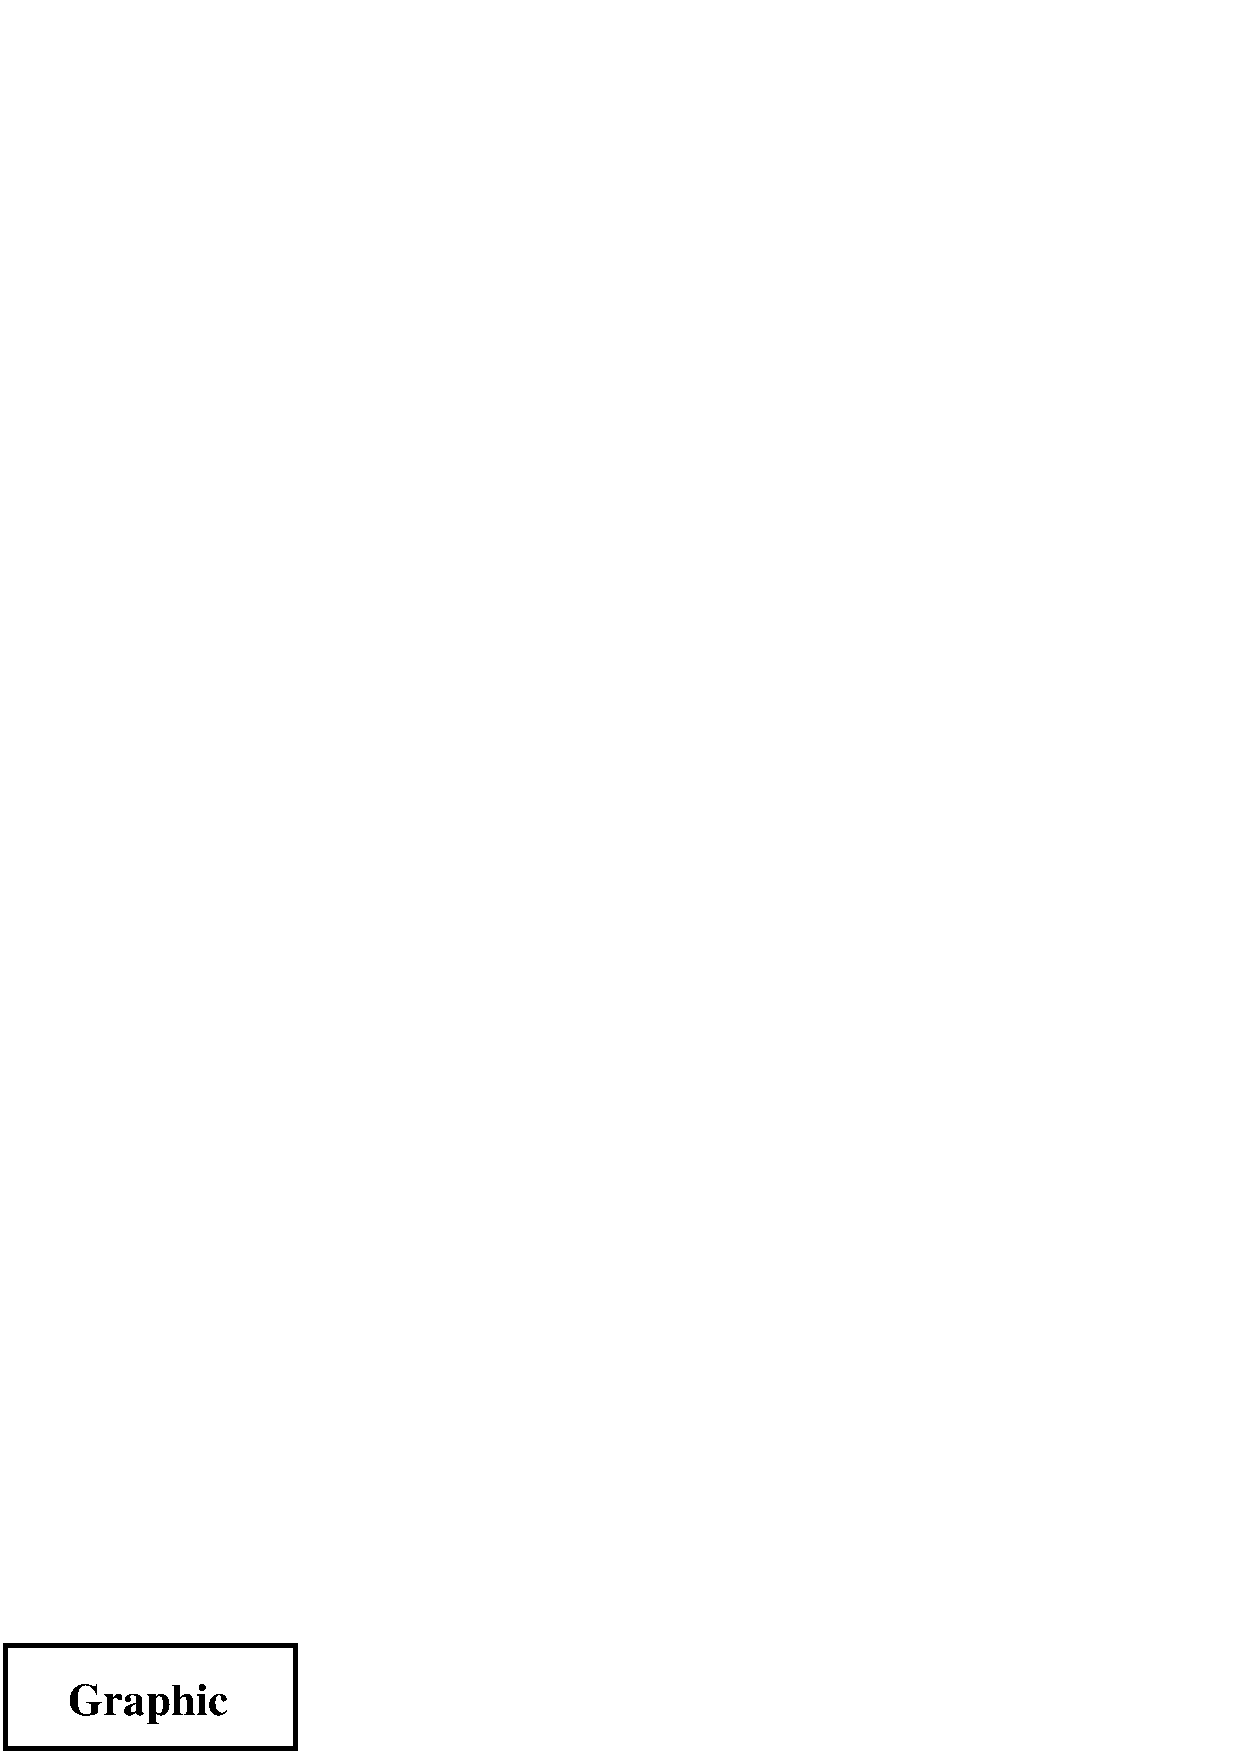
\includegraphics[width=1.5in]{graphic}}
	\caption{Two Subfigures}
	\label{fig:subfig} %% label for entire figure
\end{figure}
\end{lstlisting}
生成图~\ref{fig:subfig}。
表~\ref{tab:subfigref} 展示了用于如何引用图~\ref{fig:subfig} 中子图的命令。

\begin{figure}
	\centering
	%%----start of first subfigure----
	\subfloat[Small Box with a Long Caption]{
		\label{fig:subfig:a} %% label for first subfigure
		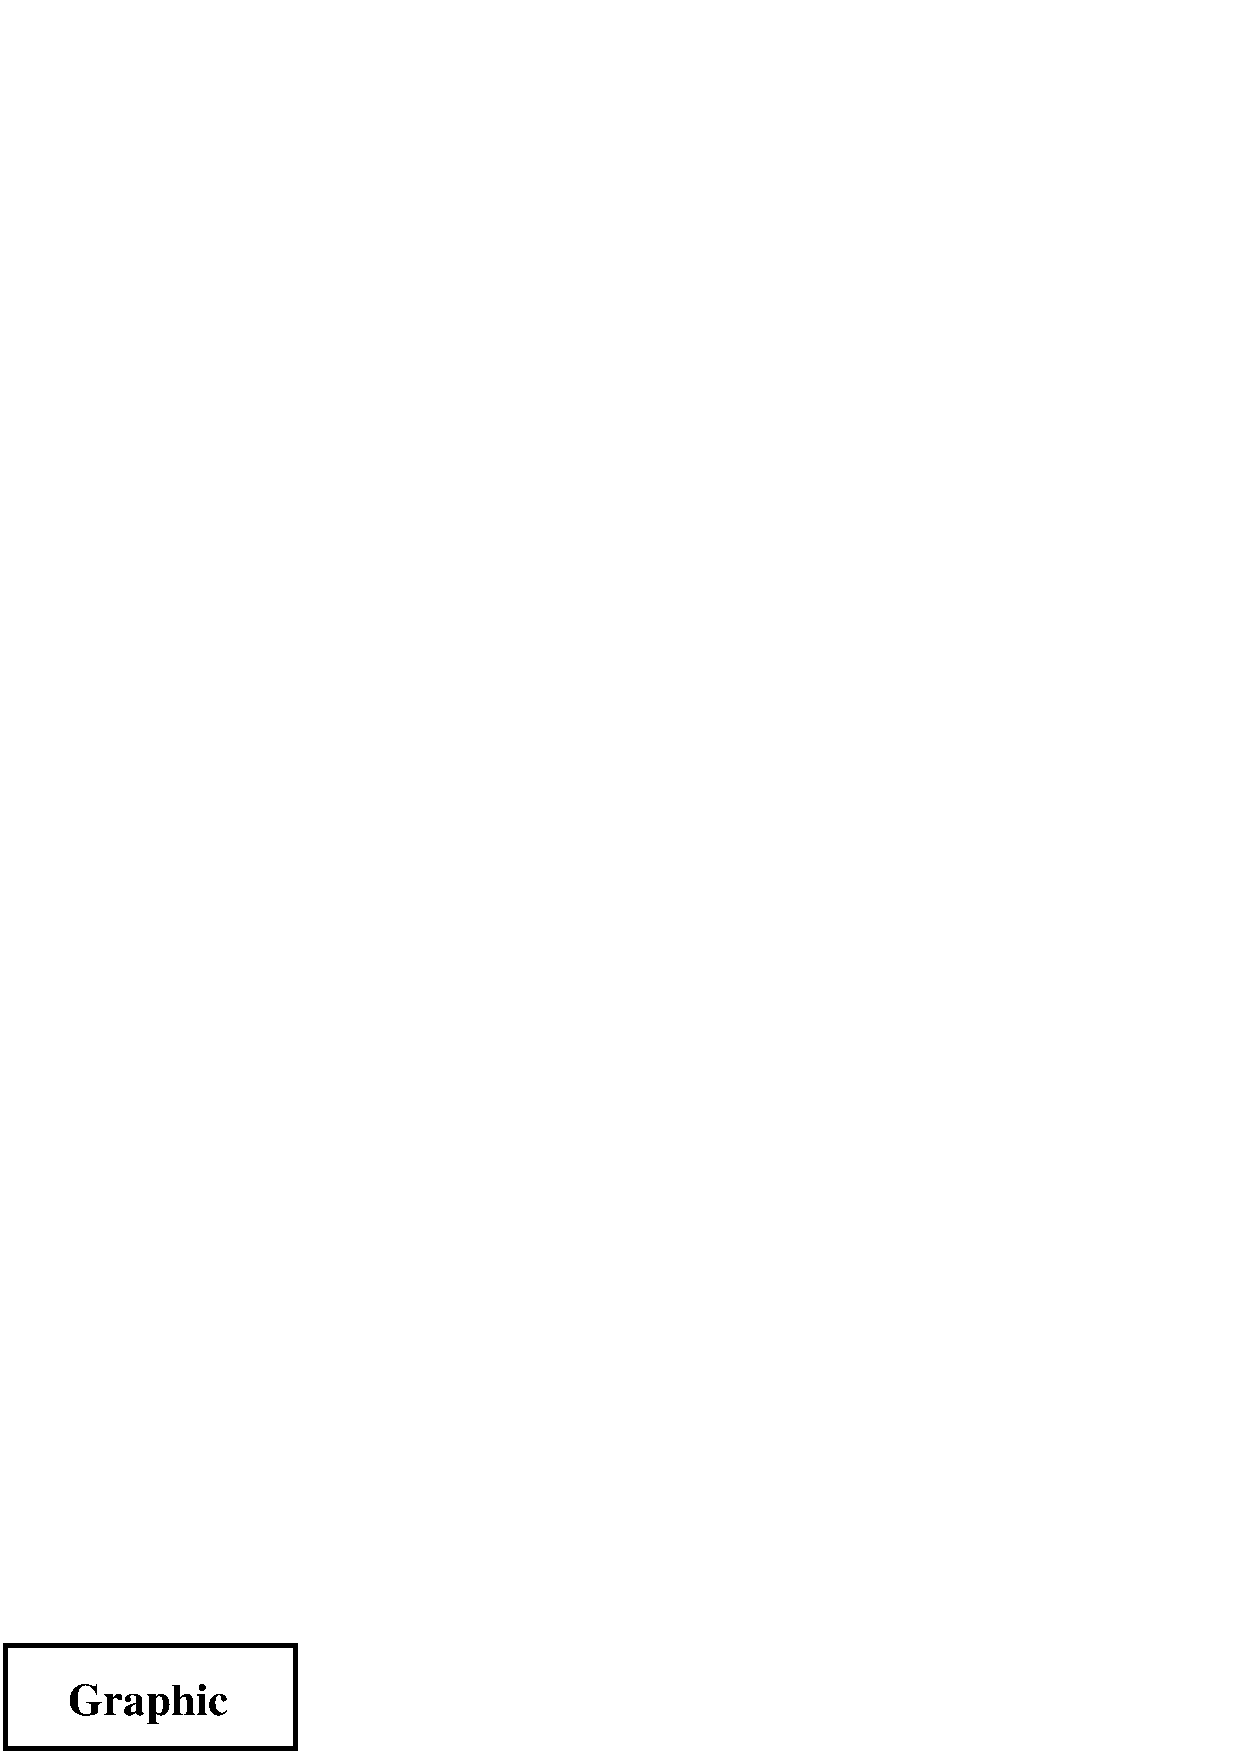
\includegraphics[width=1.0in]{graphic}}
	\hspace{1in}
	%%----start of second subfigure----
	\subfloat[Big Box]{
		\label{fig:subfig:b} %% label for second subfigure
		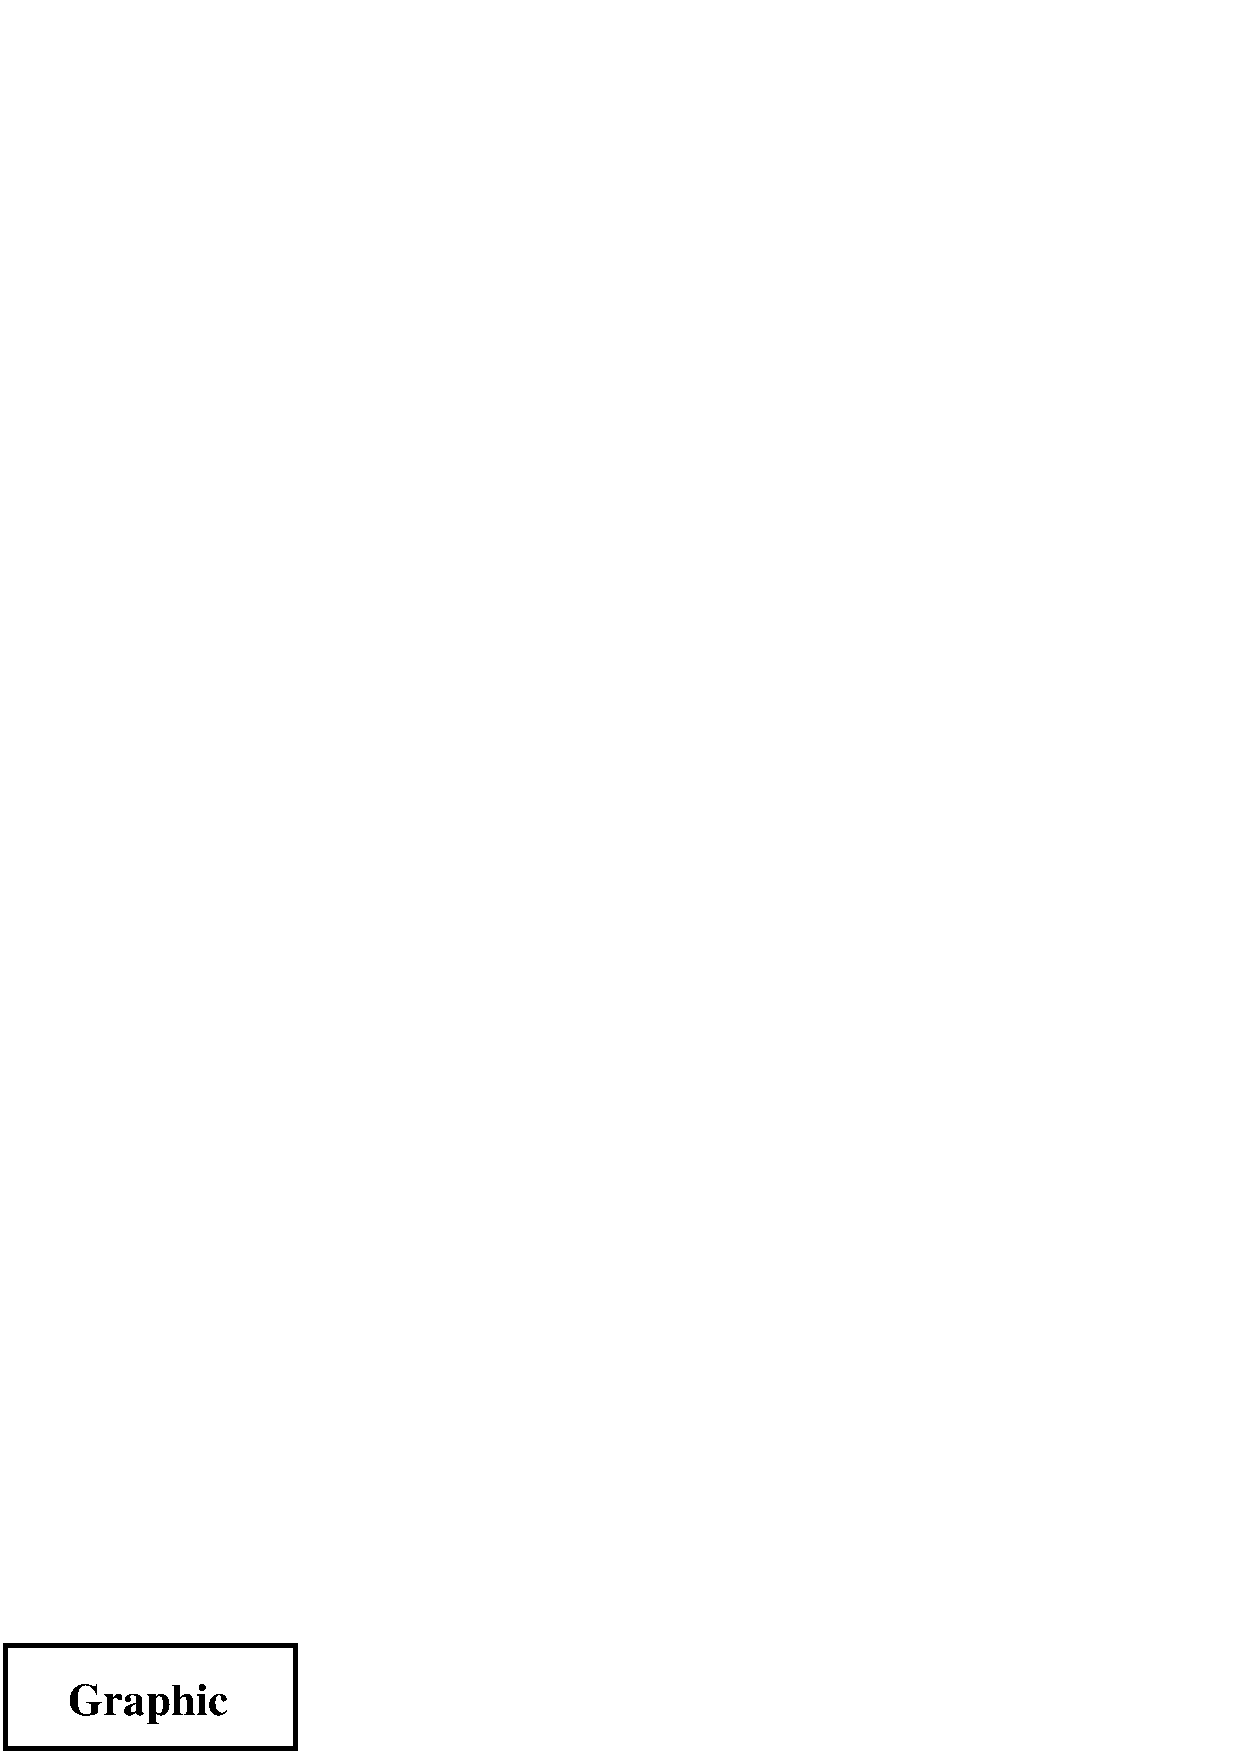
\includegraphics[width=1.5in]{graphic}}
	\caption{Two Subfigures}
	\label{fig:subfig} %% label for entire figure
\end{figure}

\begin{table}
	\centering
	\caption{图~\ref{fig:subfig} 的子图引用命令及其结果}
	\begin{tabular}{lc}
		\toprule
		引用命令 & 输出 \\
		\midrule
		\cmdonearg{subref}{fig:subfig:a} & \subref{fig:subfig:a} \\
		\cmdonearg{subref*}{fig:subfig:a} & \subref*{fig:subfig:a} \\
		\cmdonearg{ref}{fig:subfig:a} & \subref*{fig:subfig:a} \\
		\cmdonearg{subref}{fig:subfig:b} & \subref{fig:subfig:b} \\
		\cmdonearg{subref*}{fig:subfig:b} & \subref*{fig:subfig:b} \\
		\cmdonearg{ref}{fig:subfig:b} & \ref{fig:subfig:b} \\
		\cmdonearg{ref}{fig:subfig} & \ref{fig:subfig} \\
		\bottomrule
	\end{tabular}
\end{table}

\subsubsection{子图中的小页环境}

由于子图~\ref{fig:subfig:a} 只包含 \cmd{includegraphics} 命令,
因此子图~\ref{fig:subfig:a} 的标题宽度取决于插入图片的宽度。
如果子图中包含了小页环境,那么标题就可以和小页宽度一样了。
例如,
\begin{lstlisting}
\begin{figure}
	\subfloat[Small Box with a Long Caption]{
		\label{fig:mini:subfig:a} %% label for first subfigure
		\begin{minipage}[b]{0.45\linewidth}
			\centering 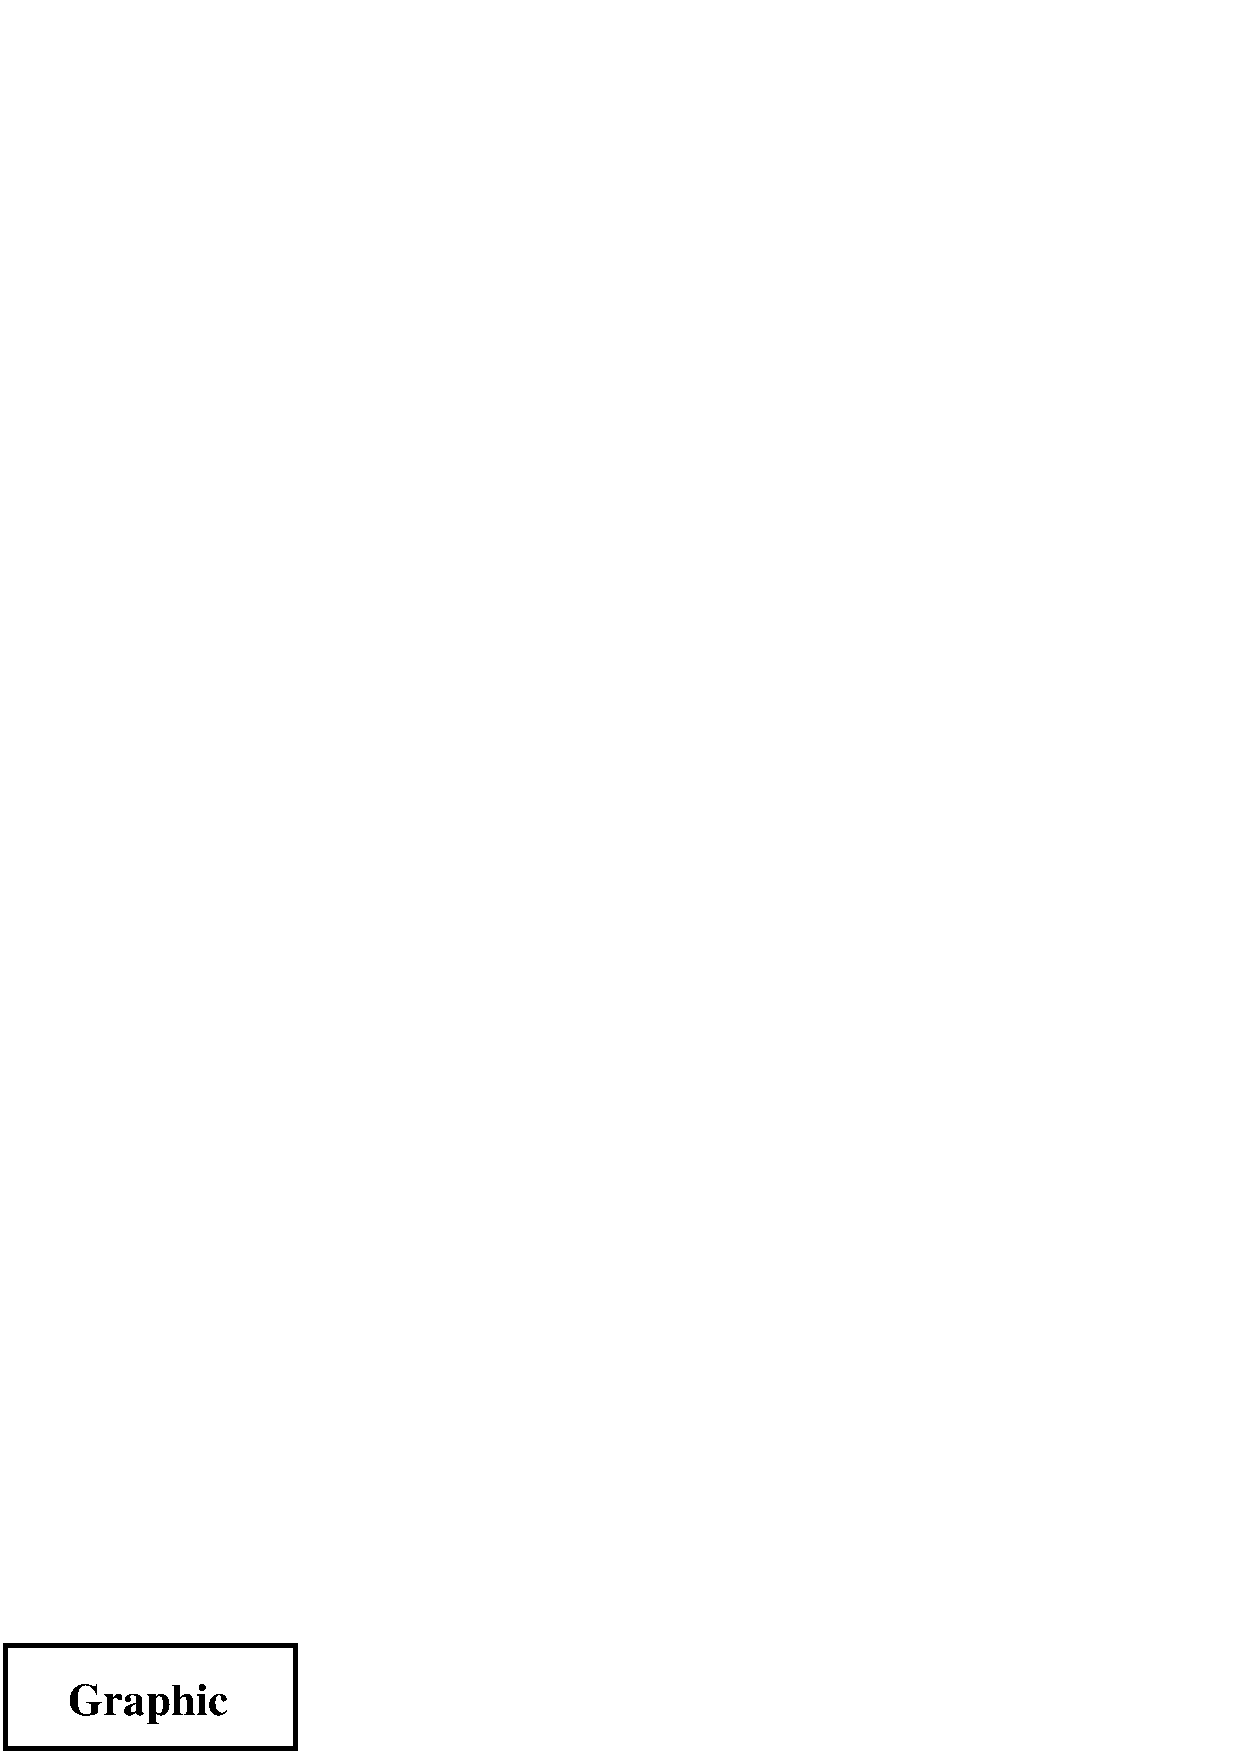
\includegraphics[width=1in]{graphic}
		\end{minipage}}%
	\hfill
	\subfloat[Big Box]{
		\label{fig:mini:subfig:b} %% label for second subfigure
		\begin{minipage}[b]{0.45\linewidth}
			\centering 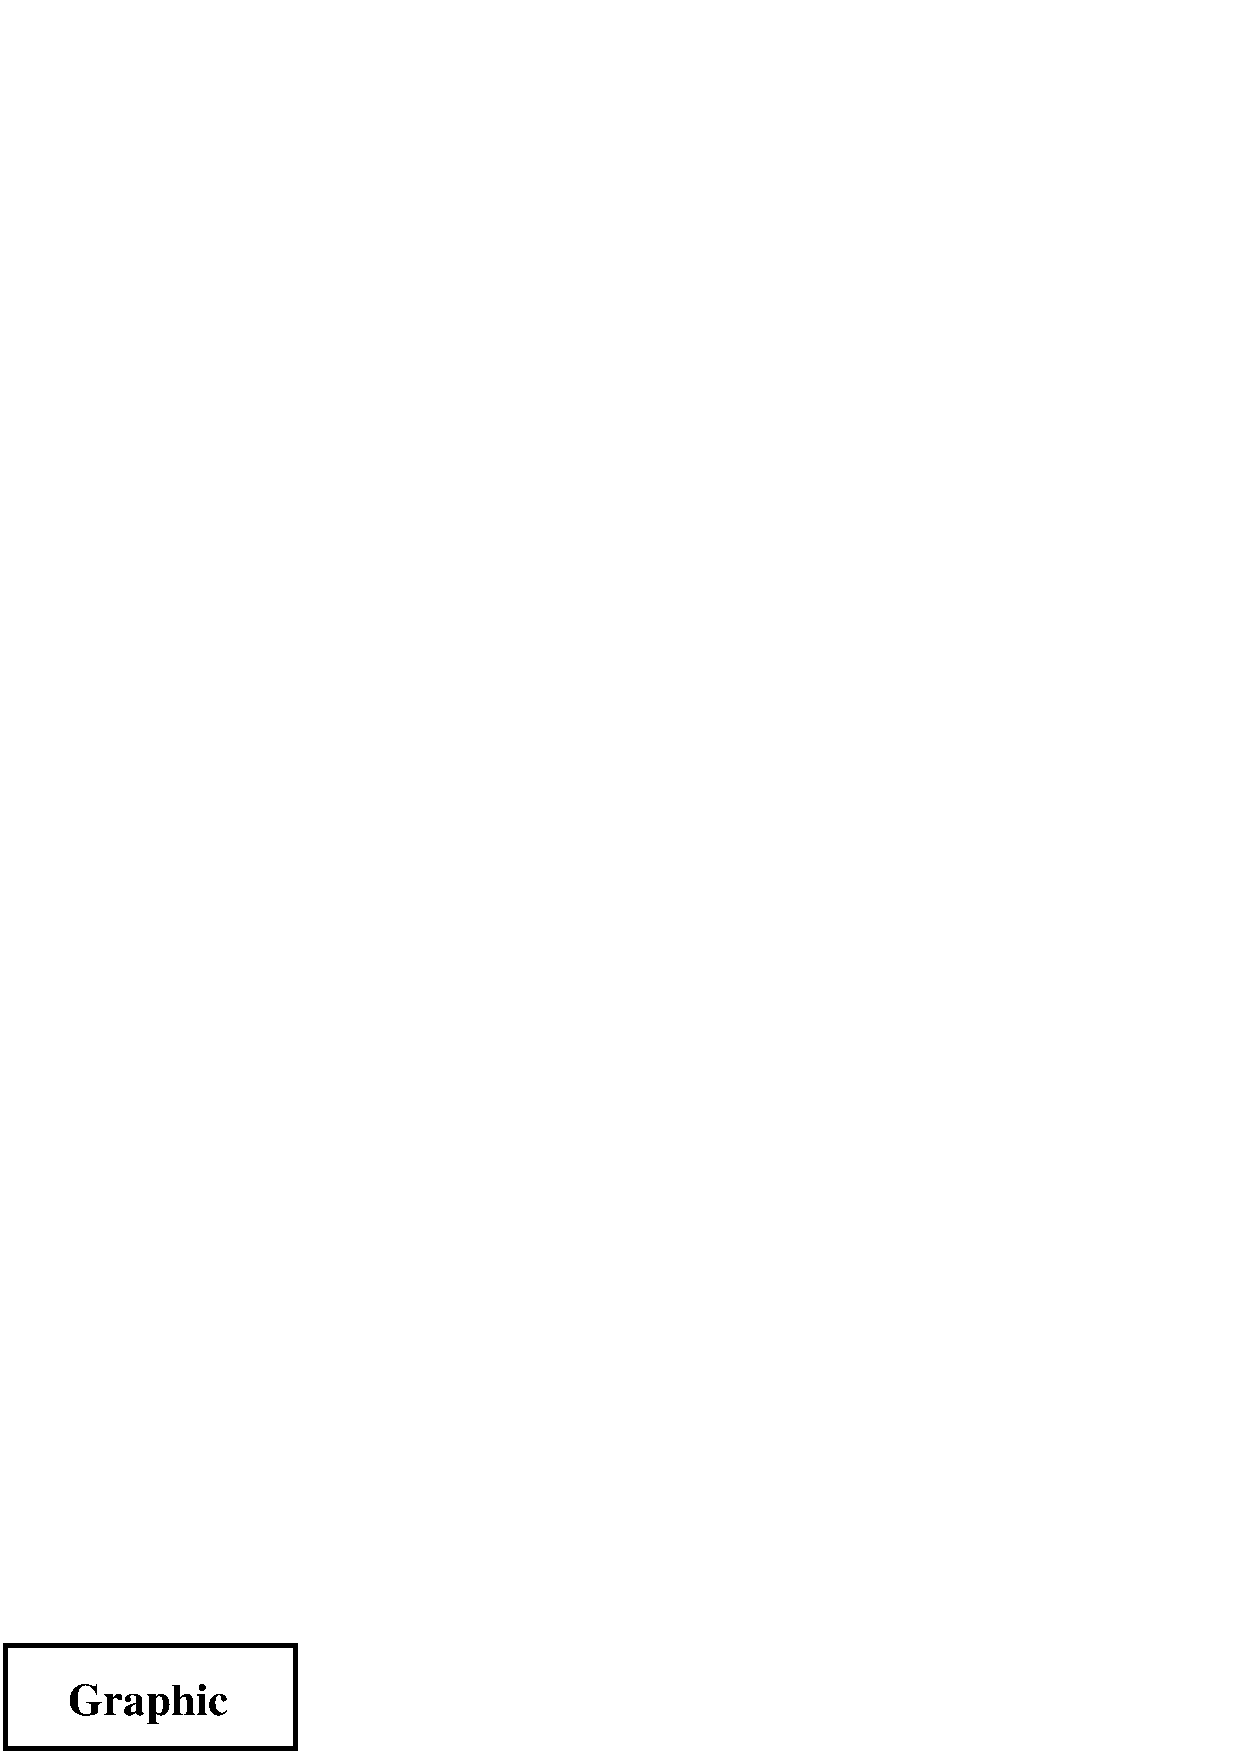
\includegraphics[width=1.5in]{graphic}
		\end{minipage}}
	\caption{Minipages Inside Subfigures}
	\label{fig:mini:subfig} %% label for entire figure
\end{figure}
\end{lstlisting}
生成图~\ref{fig:mini:subfig},其中包含了子图~\ref{fig:mini:subfig:a} 和~\ref{fig:mini:subfig:b}。

\begin{figure}
	\subfloat[Small Box with a Long Caption]{
		\label{fig:mini:subfig:a} %% label for first subfigure
		\begin{minipage}[b]{0.45\linewidth}
			\centering 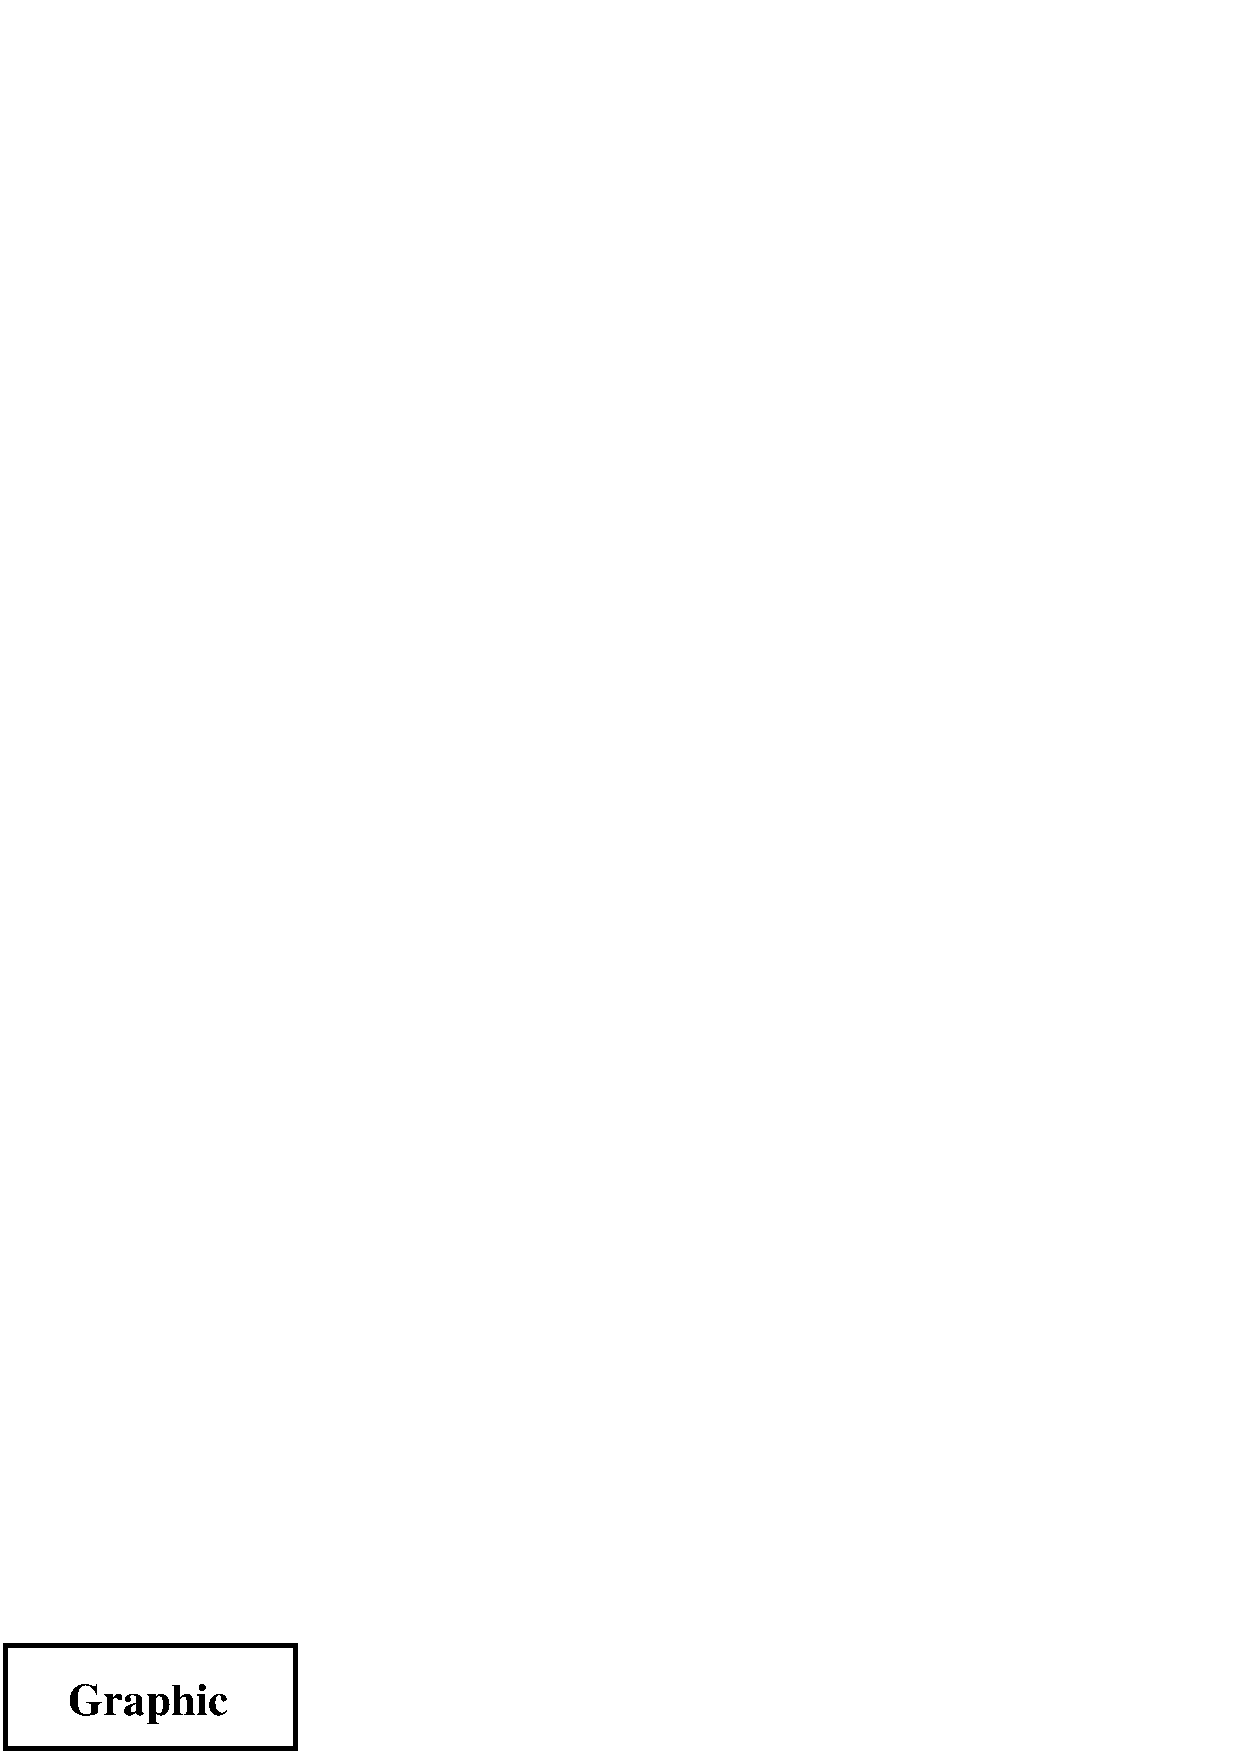
\includegraphics[width=1in]{graphic}
		\end{minipage}}%
		\hfill
		\subfloat[Big Box]{
			\label{fig:mini:subfig:b} %% label for second subfigure
			\begin{minipage}[b]{0.45\linewidth}
				\centering 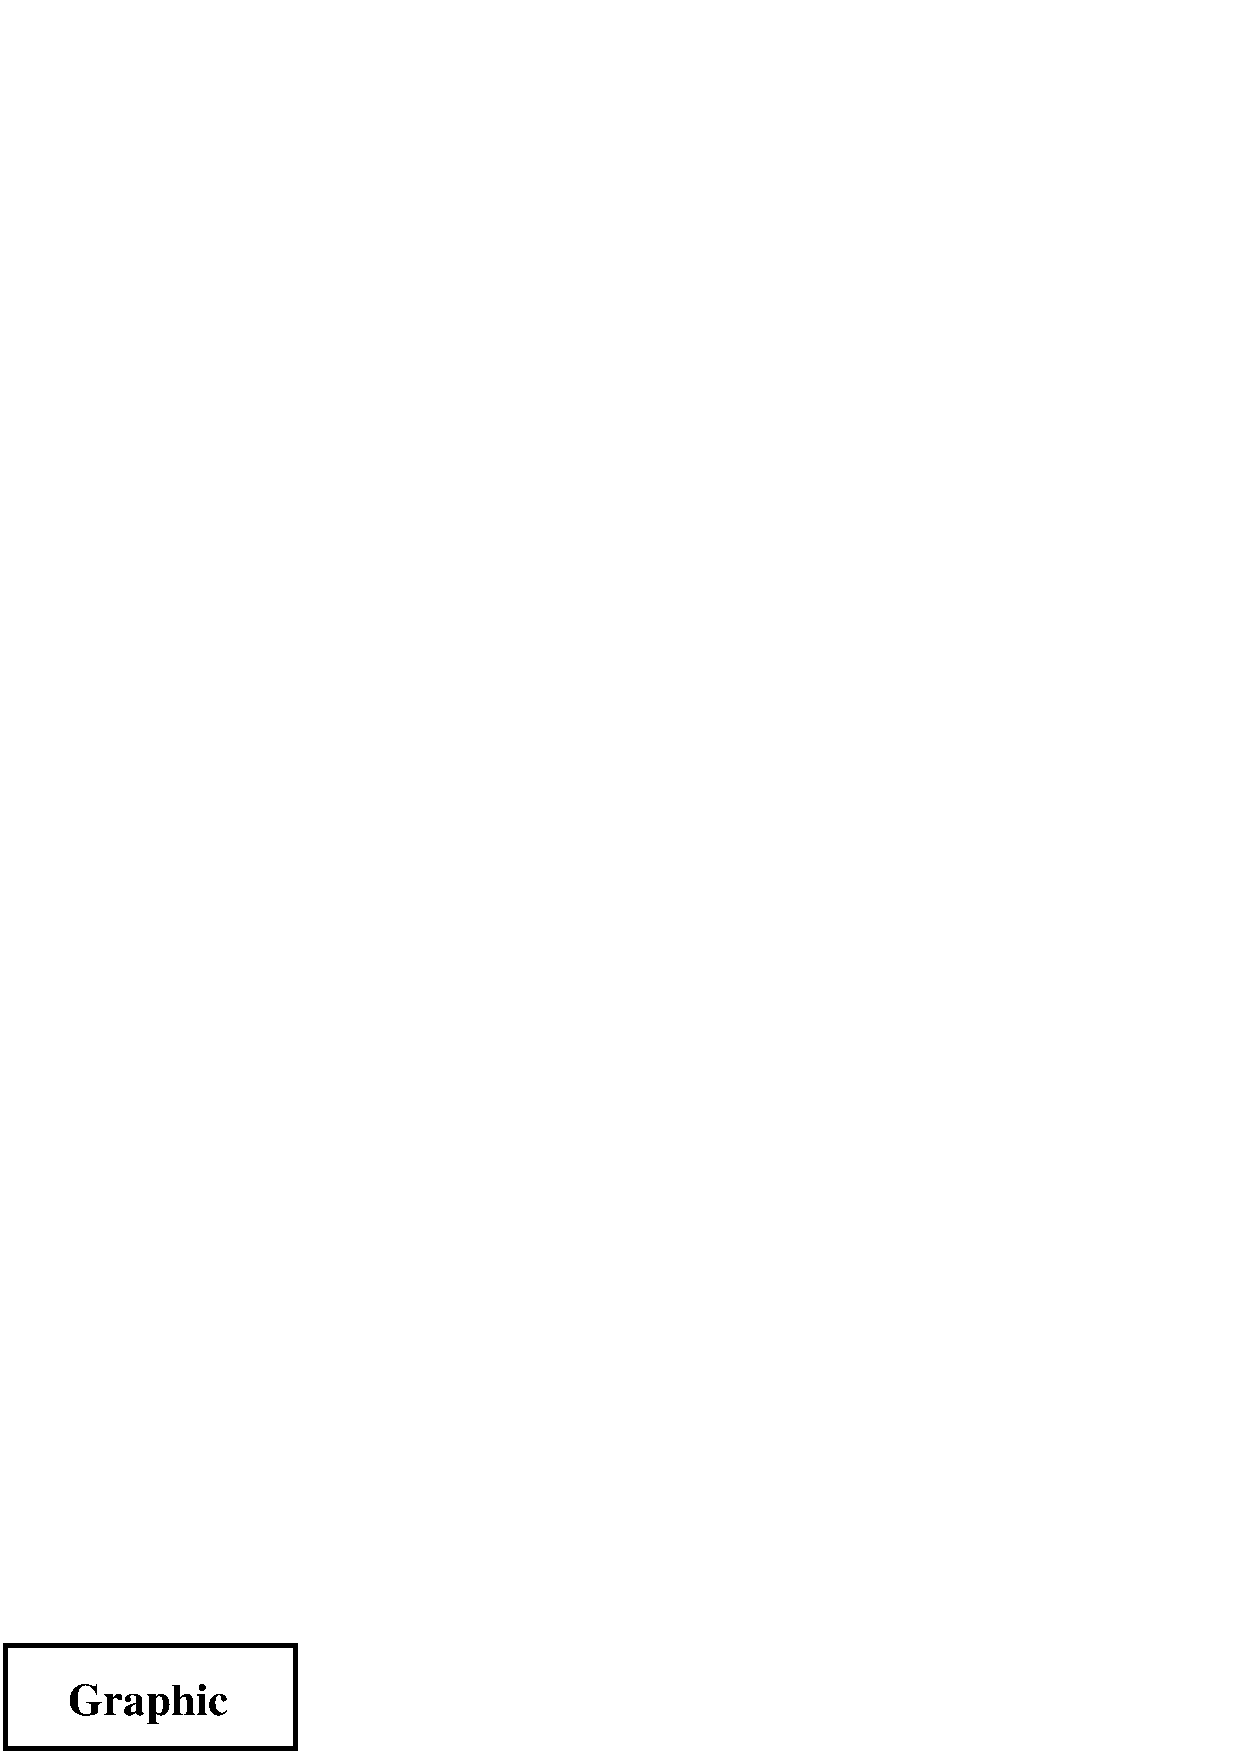
\includegraphics[width=1.5in]{graphic}
			\end{minipage}}
			\caption{Minipages Inside Subfigures}
			\label{fig:mini:subfig} %% label for entire figure
		\end{figure}

由于子图标题的宽度默认就是子图的宽度,
因此图~\ref{fig:mini:subfig} 中子图标题的宽度大于图~\ref{fig:subfig} 中的子图标题。
这是因为图~\ref{fig:subfig} 中的子图只包含图像,
而图~\ref{fig:mini:subfig} 中的子图包含了宽度为 $0.5\text{\cmd{linewidth}}$ 的小页环境。

========================================
\section{Separate Minipages for Captions}


在图~\ref{fig:side:a}~和~\ref{fig:side:b}中,并列的小页环境使用了
~\texttt{[t]}~选项,使得两幅图形的基线对齐。这对于非旋转的图形
没有任何问题,而且使得两标题的顶部对齐。不过,如果图形的底部
不对齐的话(如其中一图形被旋转),就会发生问题。例如:
\begin{Verbatim}[xleftmargin=1cm]
\begin{figure} 
\centering 
\begin{minipage}[t]{.33\textwidth} 
\centering 
\includegraphics[width=2cm]{graphic.eps} 
\caption{Box with a Long Caption} 
\end{minipage}% 
\begin{minipage}[t]{.33\textwidth} 
\centering 
\includegraphics[width=2cm,angle=-30]{graphic.eps} 
\caption{Rotated Box} 
\end{minipage}% 
\end{figure}
\end{Verbatim}
生成图~\ref{fig:mininonrot}~和~\ref{fig:minirot},我们可以看到这里
两幅图形的标题并不对齐。而若只使用小页的~\texttt{[b]}~选项,会使得标题
的最后一行对齐,并不能解决问题。

\begin{figure} 
	\centering 
	\begin{minipage}[t]{.33\textwidth} 
		\centering 
		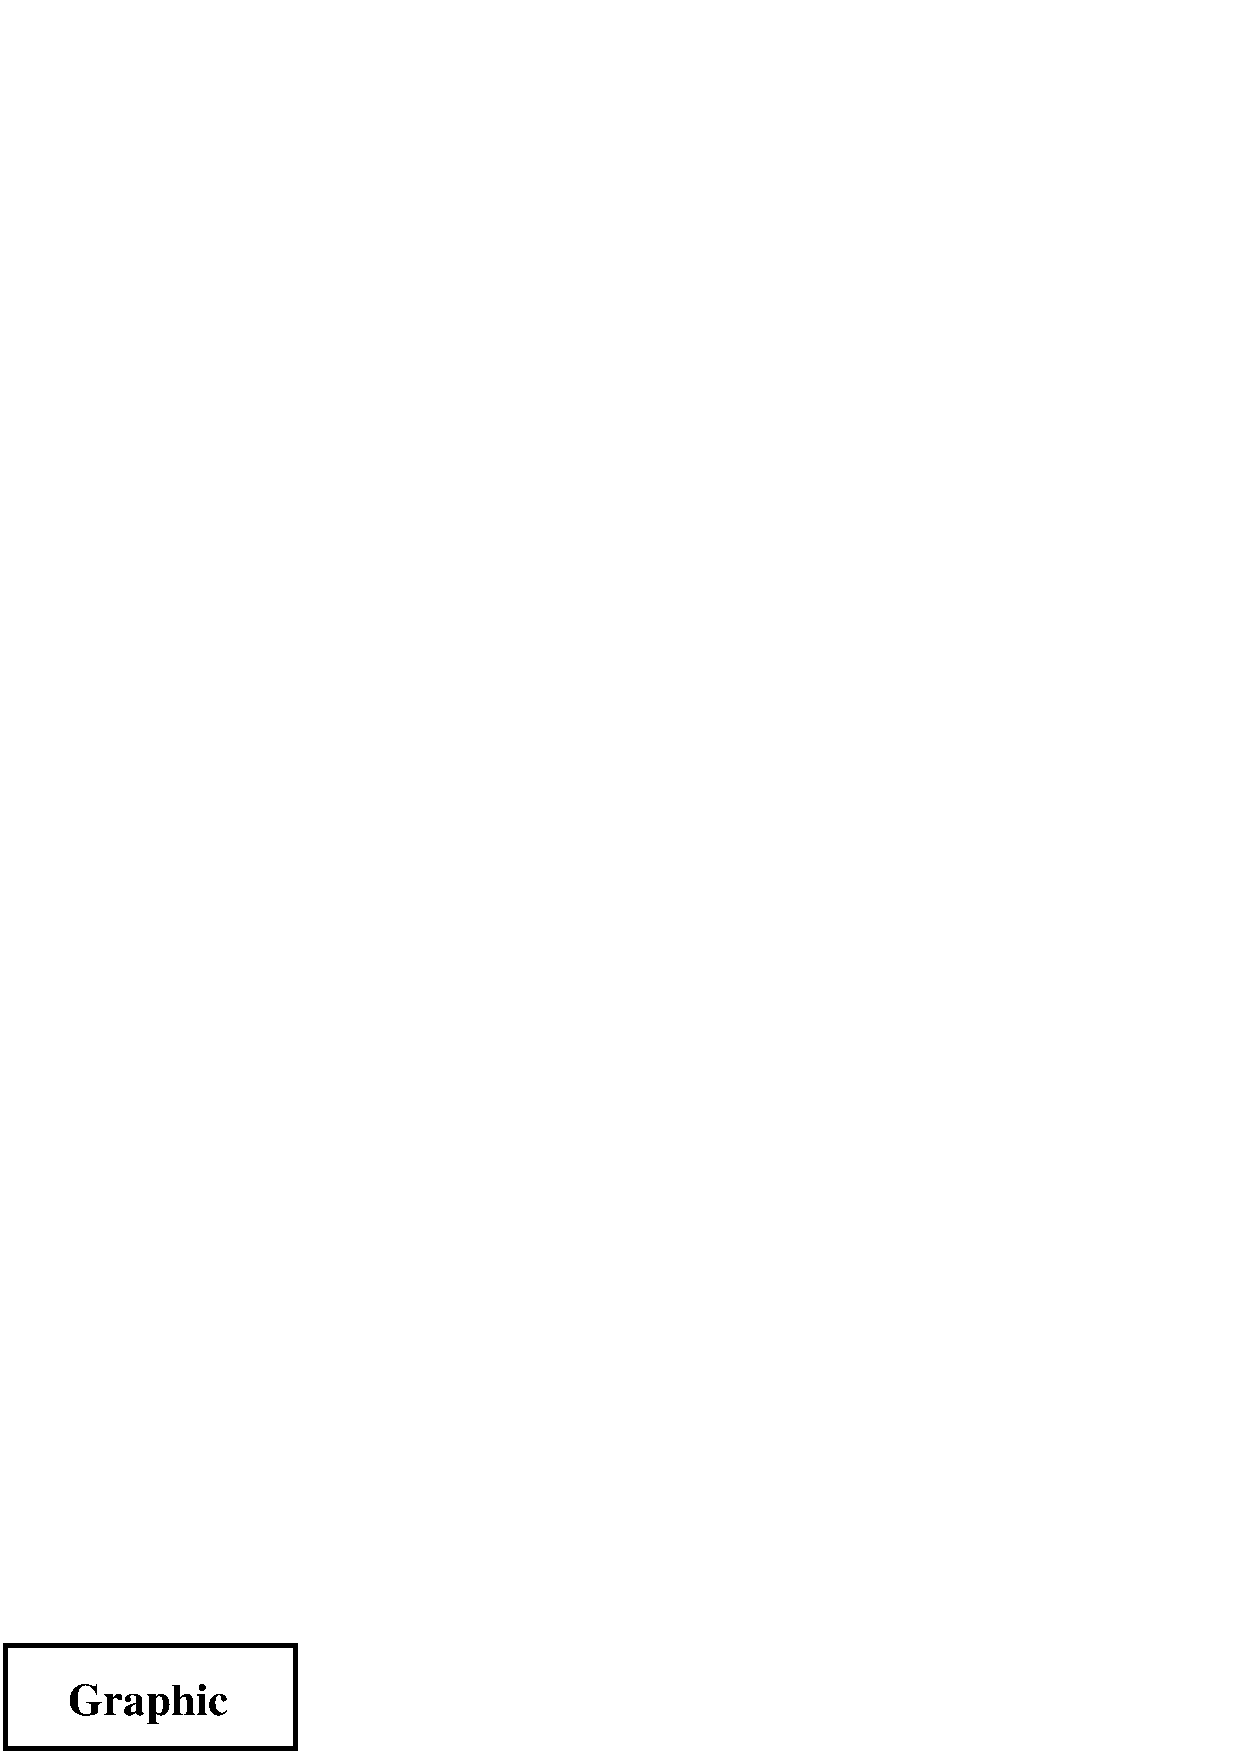
\includegraphics[width=2cm]{graphic} 
		\caption{Box with a Long Caption}\label{fig:mininonrot} 
	\end{minipage}%   
	\begin{minipage}[t]{.33\textwidth} 
		\centering 
		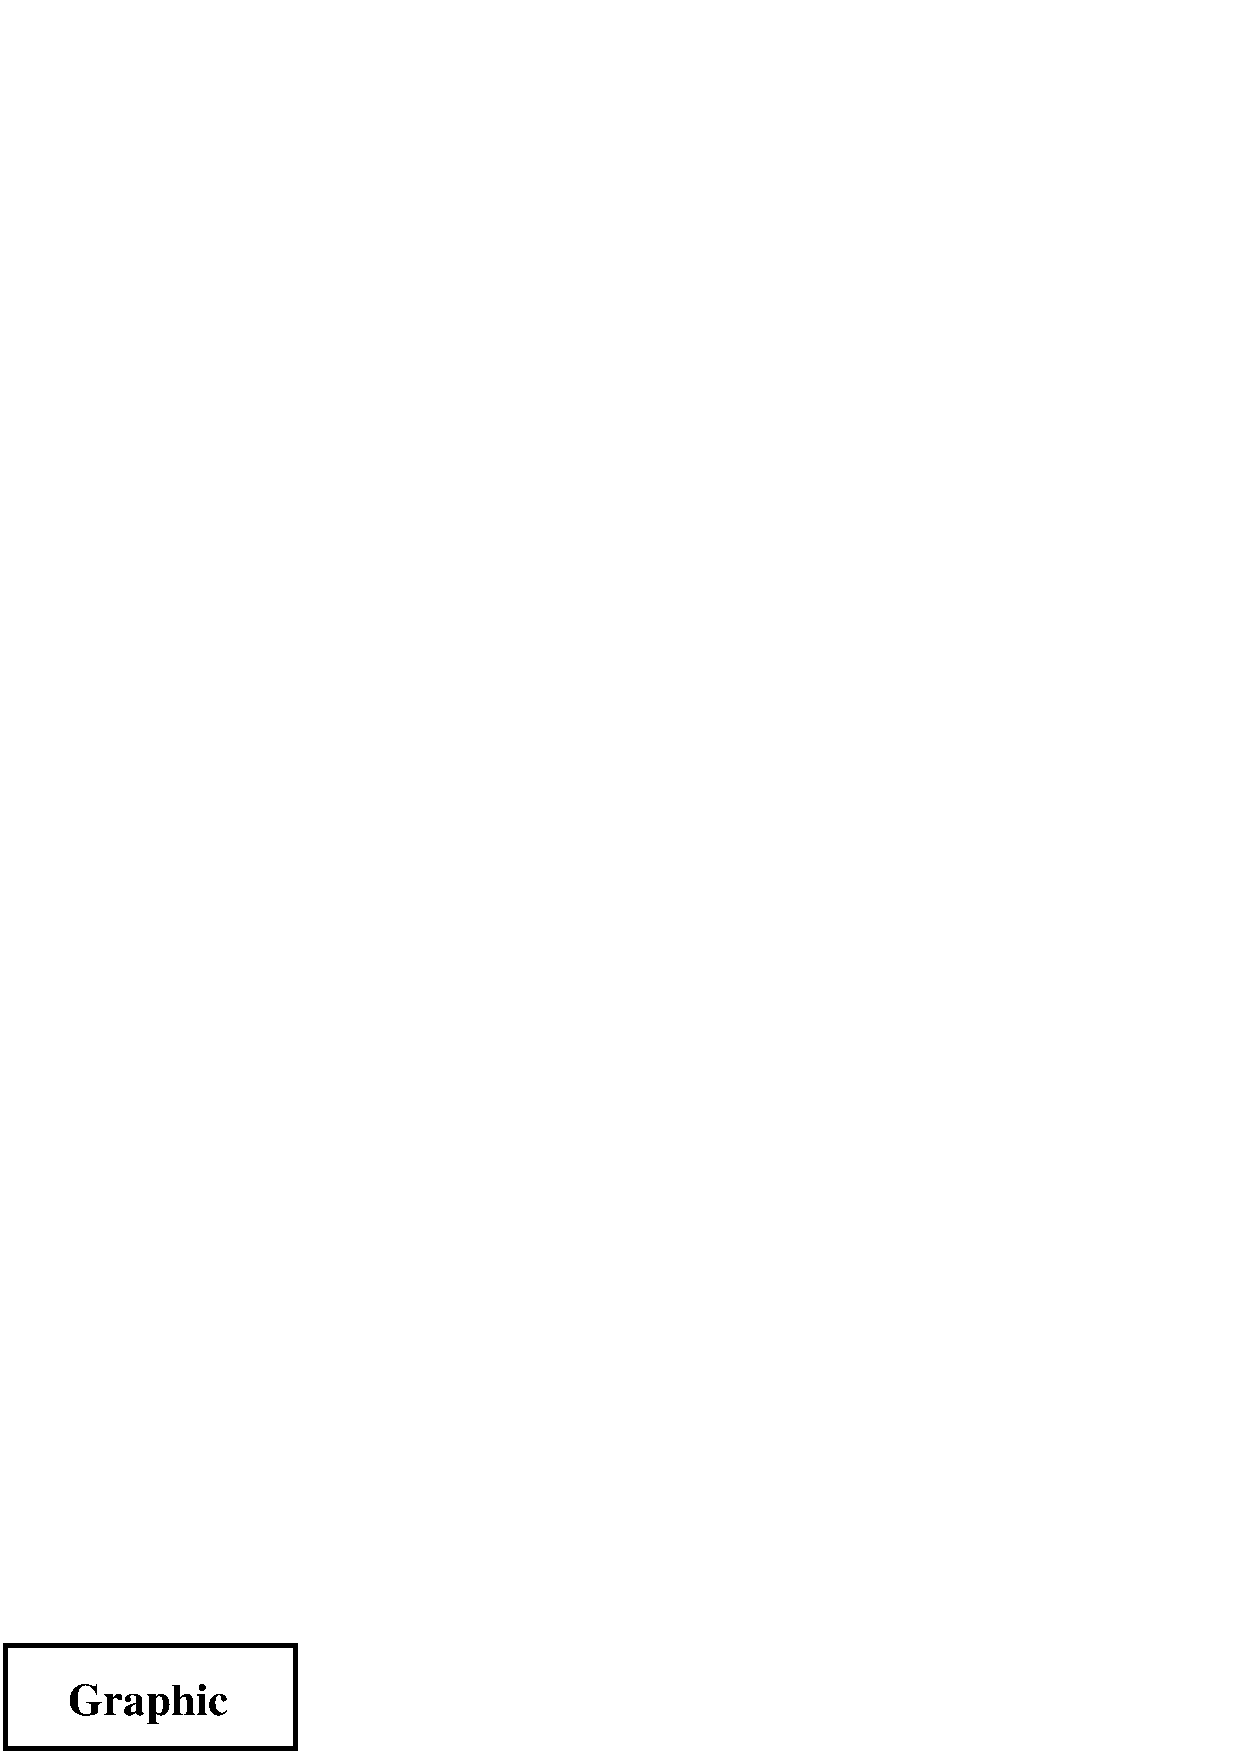
\includegraphics[width=2cm,angle=-30]{graphic} 
		\caption{Rotated Box}\label{fig:minirot} 
	\end{minipage}% 
\end{figure}

一种解决办法是在小页环境中把图形和标题分开放到两行中:第一行放置图形,
第二行放置标题。例如:
\begin{Verbatim}[xleftmargin=1cm]
\begin{figure} 
\centering 
\begin{minipage}[b]{.33\textwidth} 
\centering 
\includegraphics[width=2cm]{graphic.eps} 
\end{minipage}% 
\begin{minipage}[b]{.33\textwidth} 
\centering 
\includegraphics[width=2cm,angle=-30]{graphic.eps} 
\end{minipage}\\[-10pt] 
\begin{minipage}[t]{.33\textwidth} 
\caption{Box with a Long Caption} 
\end{minipage}% 
\begin{minipage}[t]{.33\textwidth} 
\caption{Rotated Box} 
\end{minipage}% 
\end{figure}
\end{Verbatim}
生成的图~\ref{fig:mininonrot:a}~和~\ref{fig:minirot:a}~中,图形的基
线和标题的第一行分别对齐。

\begin{figure}
	\centering
	\begin{minipage}[b]{.33\textwidth}
		\centering
		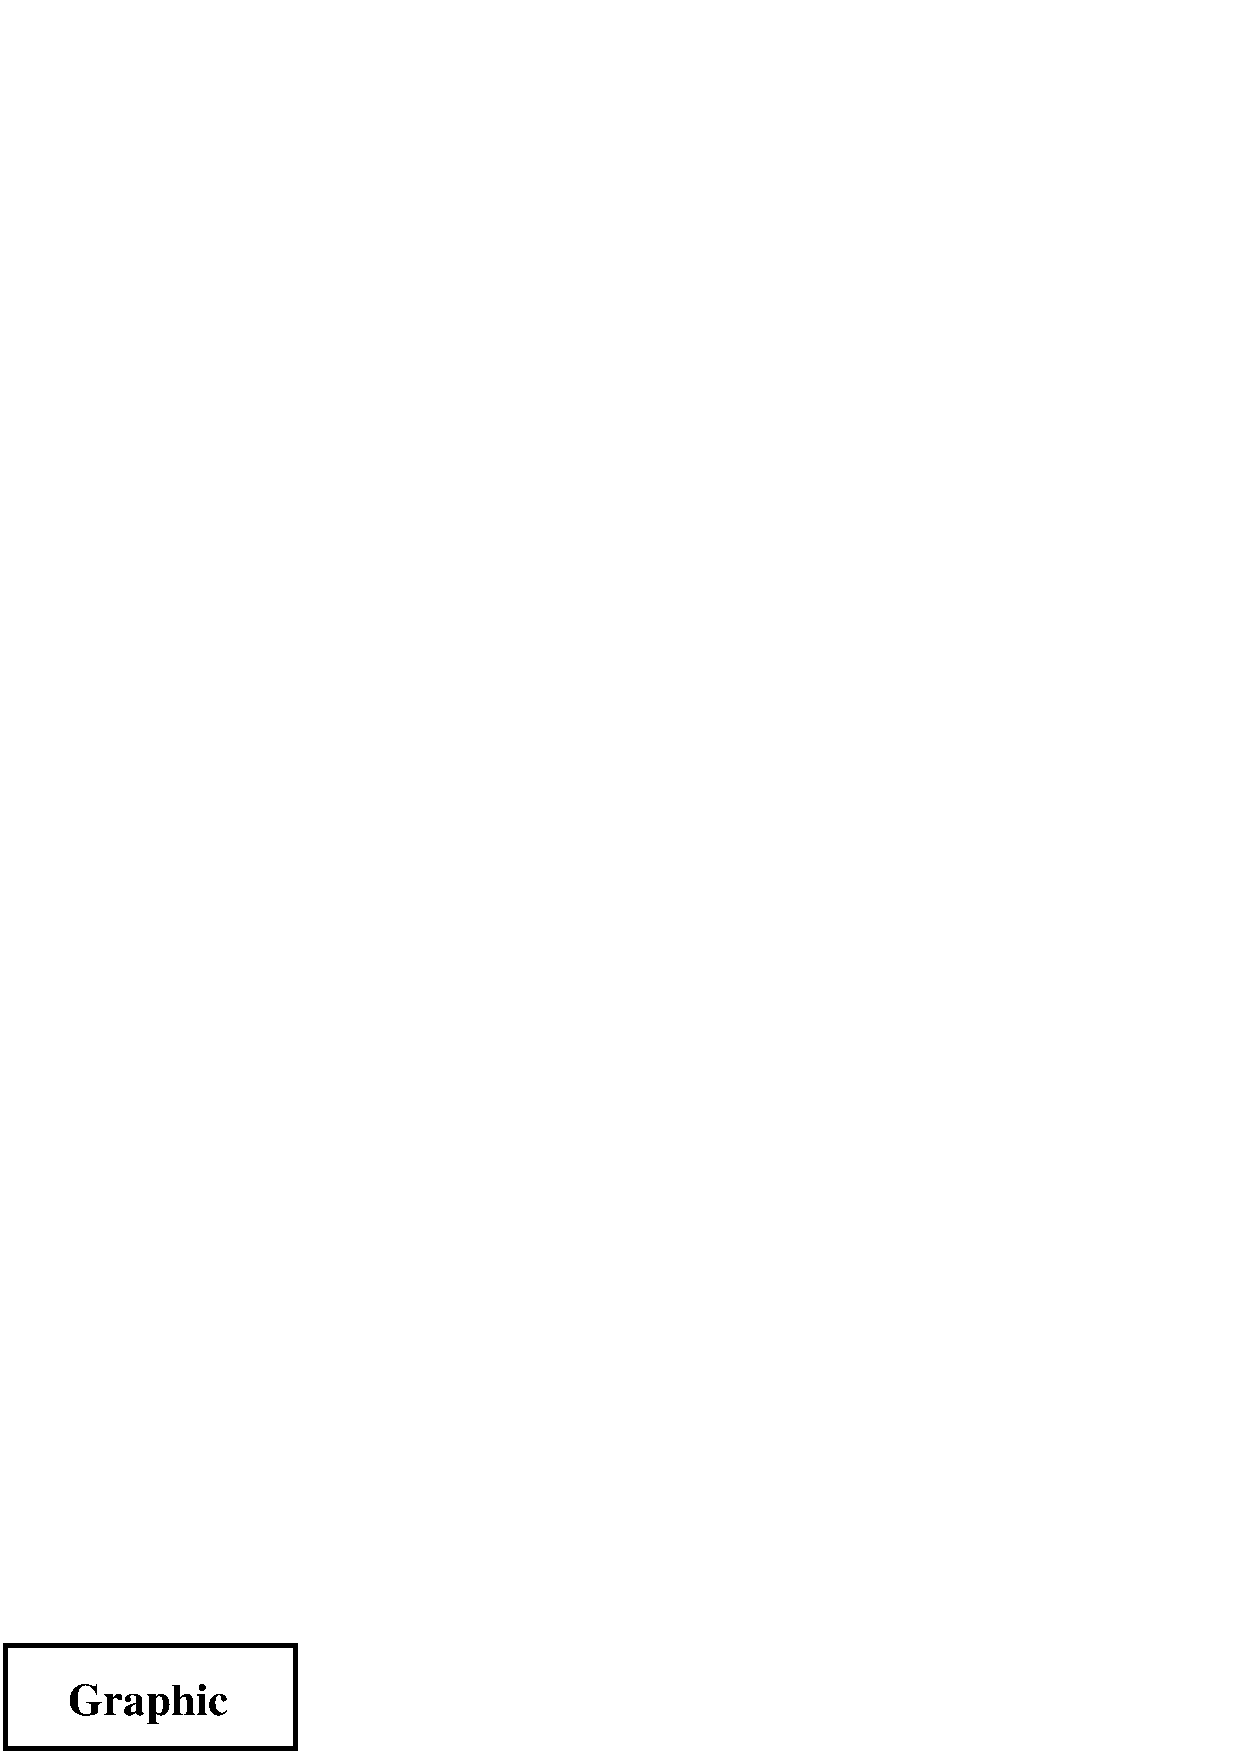
\includegraphics[width=2cm]{graphic}
	\end{minipage}%
	\begin{minipage}[b]{.33\textwidth}\label{fig:mininonrot:a}
		\centering
		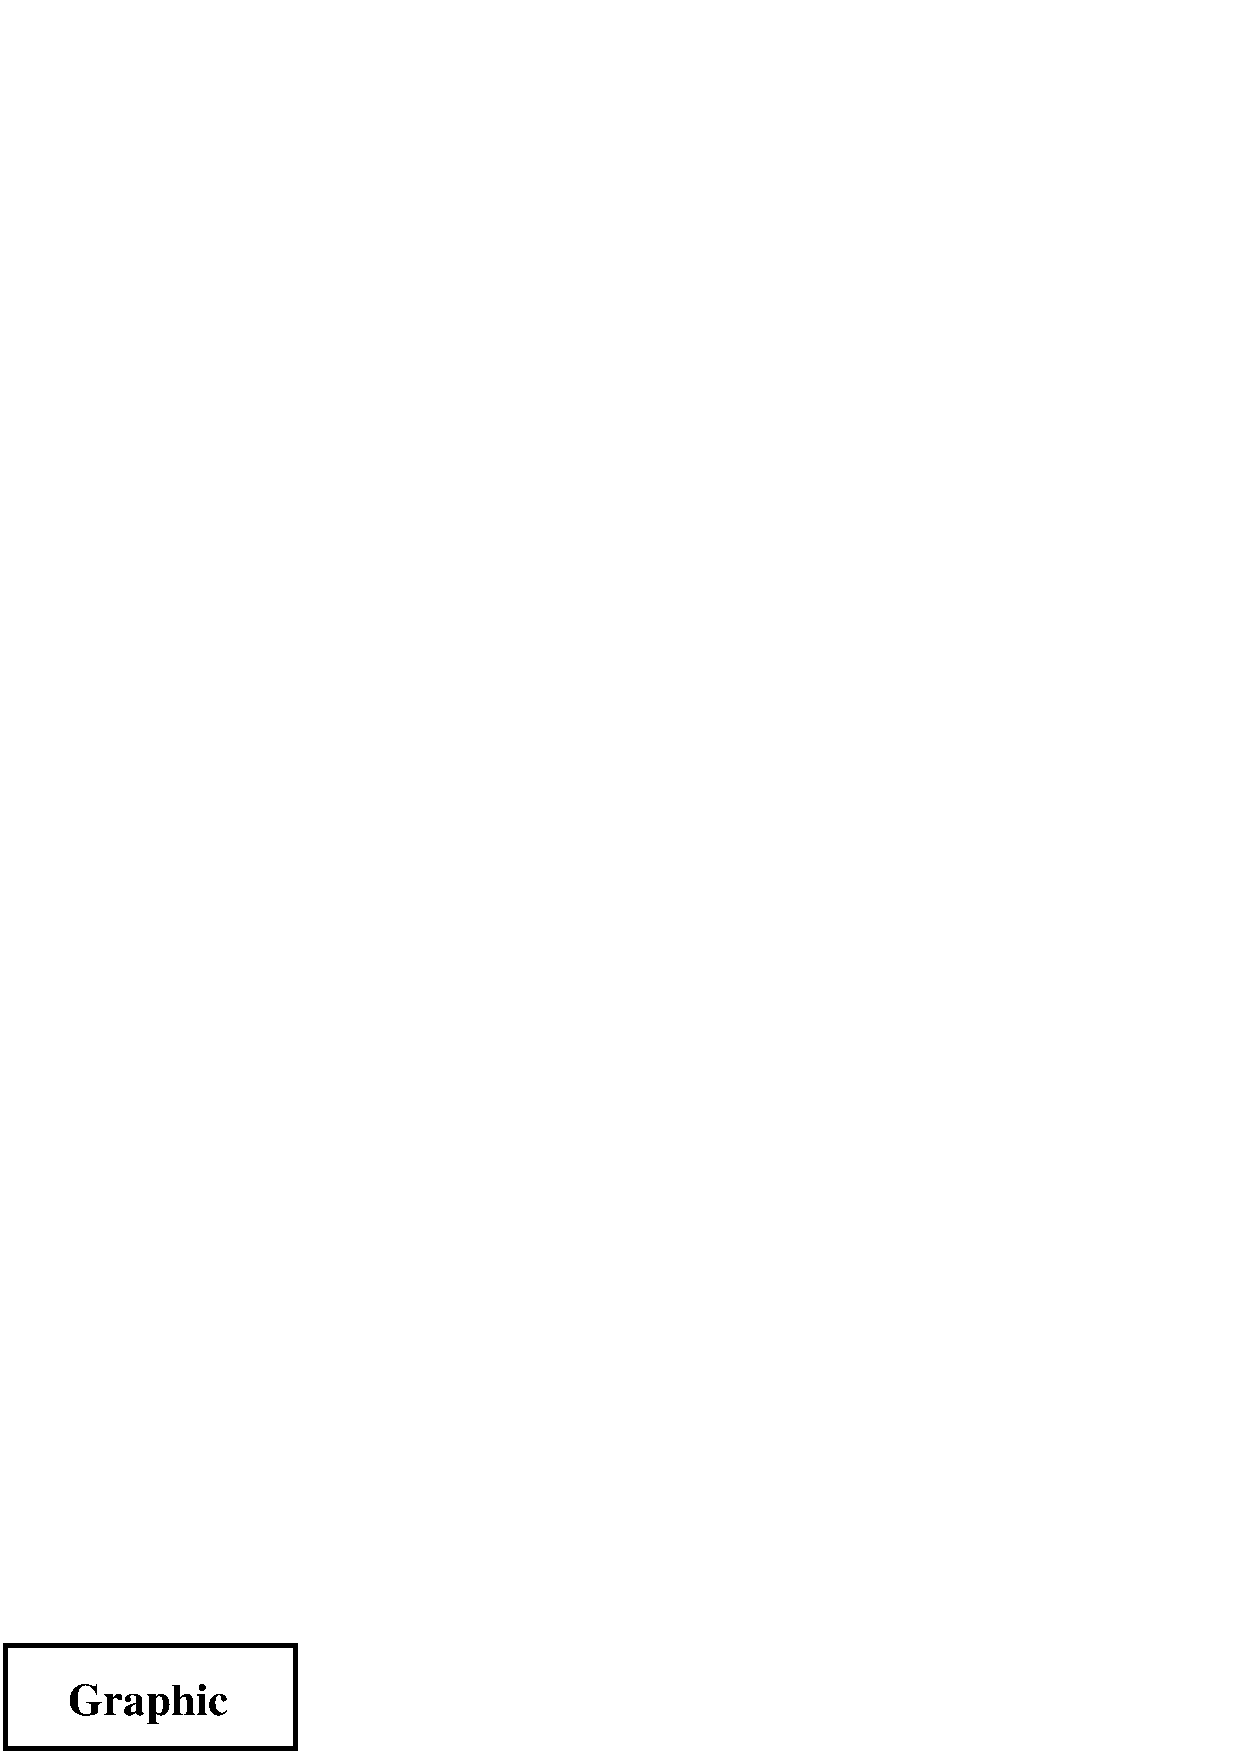
\includegraphics[width=2cm,angle=-30]{graphic}
	\end{minipage}\\[-10pt]
	\begin{minipage}[t]{.33\textwidth}
		\caption{Box with a Long Caption}
	\end{minipage}%
	\begin{minipage}[t]{.33\textwidth}
		\caption{Rotated Box}\label{fig:minirot:a}
	\end{minipage}%
\end{figure}

\noindent在这个例子中,需要注意:
\begin{itemize}
	\item 在最后一幅图后面用~\cmd{\bs}~来断行,~\cmd{\bs}~的参数项
	~\texttt{[-10pt]}~使得图形与标题之间的距离比当前行距
	减少~\texttt{10pt}。这样做是让图形和标题更接近些,用户也可
	自己选用合适的值。
	\item 包含图形的小页使用~\texttt{[b]}~选项,使得它们的参考点为
	其最后一行的基线。
	\item 包含标题小页使用~\texttt{[t]}~选项,使得它们的参考点为
	其第一行的基线。
	\item 任何一个~\cmd{label}~命令都必须和它相应的~\cmd{caption}~
	命令在同一个小页中。
\end{itemize}


\section{图形与表格的平行排列}\label{sec:figuretable}

在第~\ref{chap:sidebyside}~章中,通过在一个~\texttt{figure}~环境中使用多个
~\cmd{caption}~命令来得到并列的多个图形。同样地,在一个~\texttt{table}~
环境中使用多个~\cmd{caption}~命令可将多个表格平行排列。
若想使表格和图形平行排列在一起,可使用第~\ref{chap:nonfloat}~中定义
的命令~\cmd{figcaption}~和~\cmd{tabcaption}。
例如下面的命令:
\begin{Verbatim}[xleftmargin=1cm]
\begin{figure}[htb] 
\begin{minipage}[b]{0.5\textwidth} 
\centering 
\includegraphics[width=0.8\textwidth]{graphic.eps} 
\caption{This is a Figure by a Table} 
\label{fig:by:table} 
\end{minipage}% 
\begin{minipage}[b]{0.5\textwidth} 
\centering
\begin{tabular}{|c|c|} \hline 
Day & Data \\ \hline\hline 
Monday    & 14.6 \\ 
Tuesday   & 14.3 \\ 
Wednesday & 14.2 \\ 
Thursday  & 14.5 \\ 
Friday    & 14.9 \\ \hline 
\end{tabular} 
\tabcaption{This is a Table by a Figure} 
\label{table:by:fig} 
\end{minipage} 
\end{figure}
\end{Verbatim}
用一个~\texttt{figure}~环境生成了并排放置的图~\ref{fig:by:table}~和
表~\ref{table:by:fig}。

\begin{figure}[htb]
	\begin{minipage}[b]{0.5\textwidth}
		\centering
		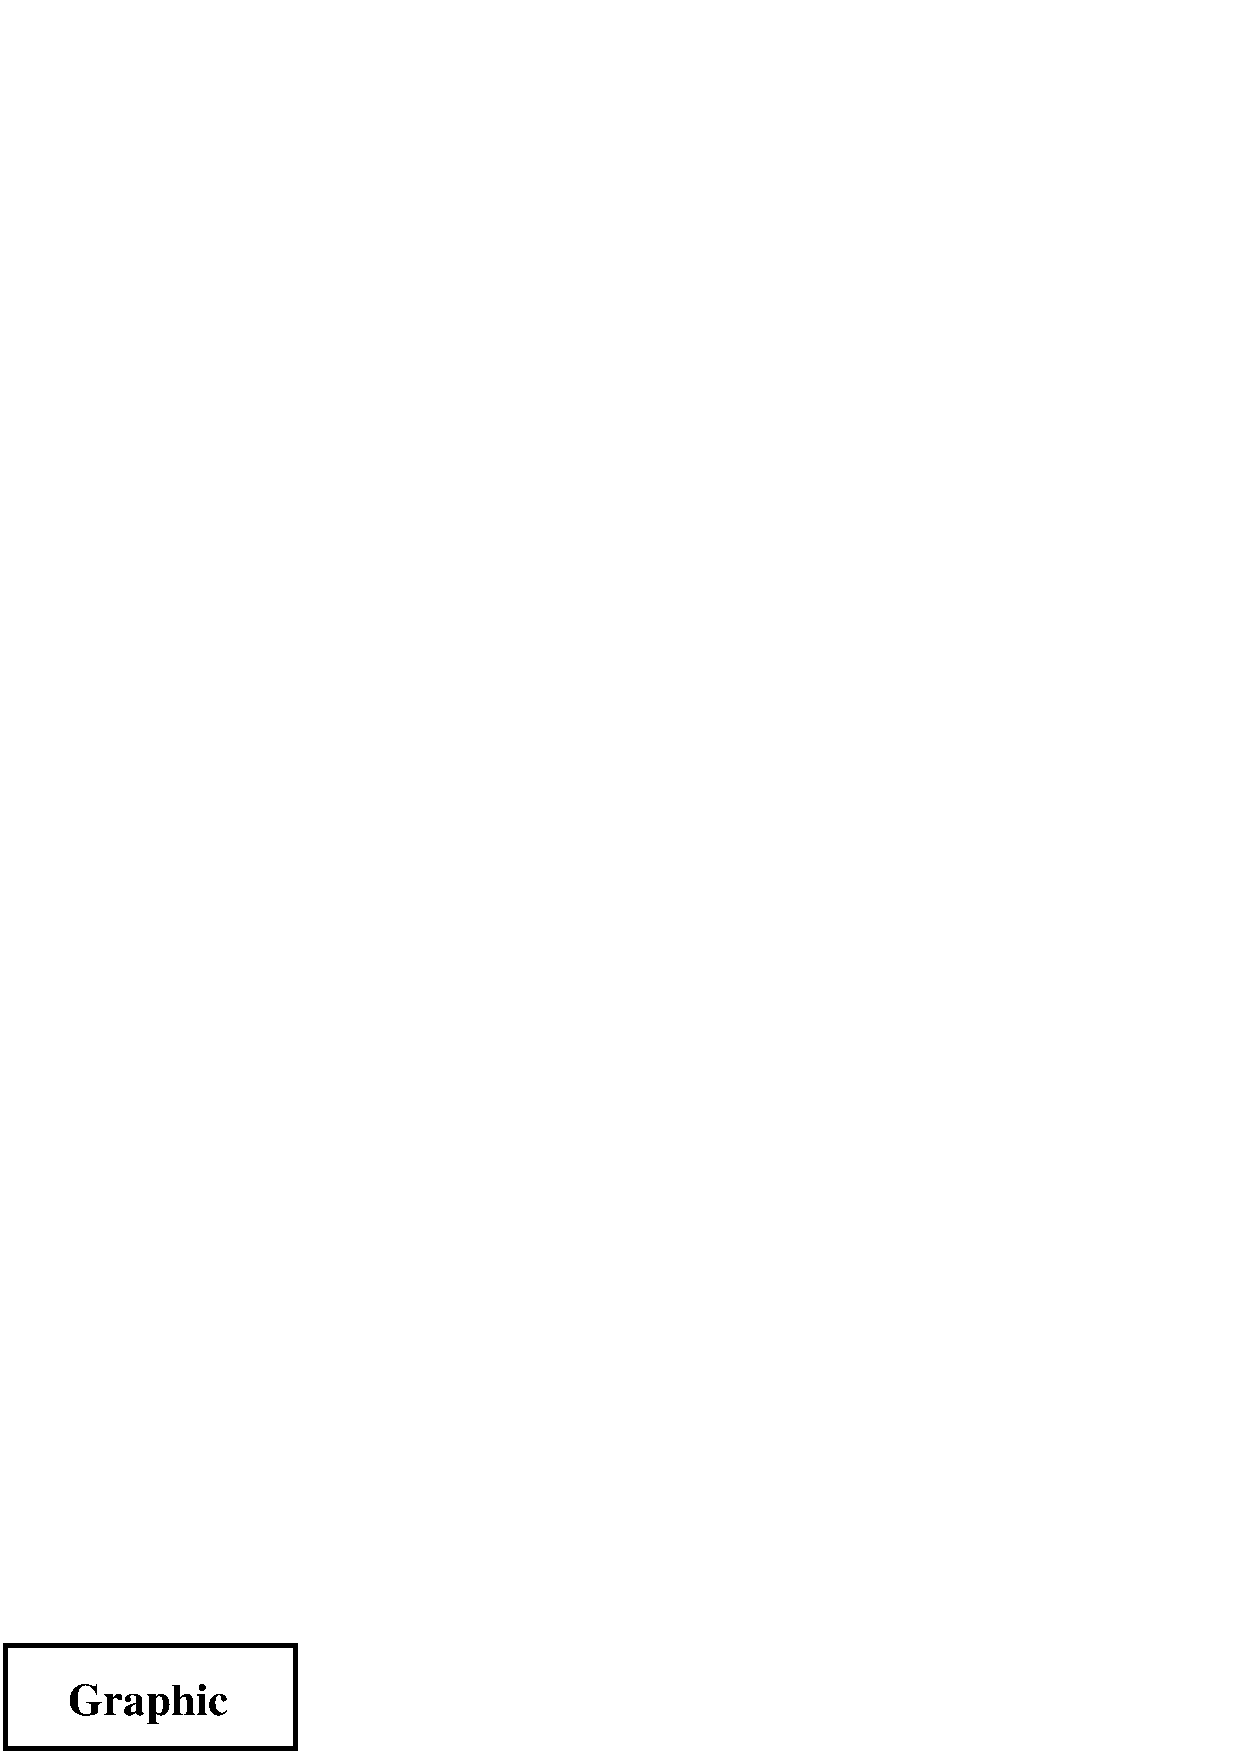
\includegraphics[width=0.8\textwidth]{graphic} 
		\caption{This is a Figure by a Table} 
		\label{fig:by:table} 
	\end{minipage}% 
	\begin{minipage}[b]{0.5\textwidth} 
		\centering
		\begin{tabular}{|c|c|} \hline
			Day & Data \\ \hline\hline
			Monday    & 14.6 \\ 
			Tuesday   & 14.3 \\
			Wednesday & 14.2 \\ 
			Thursday  & 14.5 \\ 
			Friday    & 14.9 \\ \hline
		\end{tabular}
		\tabcaption{This is a Table by a Figure} 
		\label{table:by:fig} 
	\end{minipage} 
\end{figure}

因为~\LaTeX{}~允许图形的浮动不必考虑其前后表格的顺序,所以在
~\texttt{figure}~环境中使用命令~\cmd{tabcaption}~可能会将表格
放置到尚未处理的浮动图形前面。同理,在~\texttt{table}~环境中
使用命令~\cmd{figcaption}~可能会将图形放置到尚未处理的浮动图形前面。
这种情况下,可以在图形环境前使用~\cmd{FloatBarrier}~命令来清除
其前面尚未处理的浮动图形。

\section{Placing a Table Beside a Figure}

\section{堆叠图形}

在第~\ref{chap:sidebyside}~章中,通过将几个盒子并排放置在
一行中来得到并列图形。堆叠图形(stacked graphics)也可用同样的
方法来生成。例如:
\begin{Verbatim}[xleftmargin=1cm]
\begin{figure} 
\centering 
\begin{minipage}[b]{0.3\textwidth} 
\centering 
\includegraphics[width=1in]{graphic.eps} 
\caption{Caption 1}
\end{minipage}% 
\hspace{0.04\textwidth}% 
\begin{minipage}[b]{0.3\textwidth} 
\centering 
\includegraphics[width=1in]{graphic.eps} 
\caption{Caption 2} 
\end{minipage}\\[20pt] 
\begin{minipage}[b]{0.3\textwidth} 
\centering 
\includegraphics[width=1in]{graphic.eps} 
\caption{Caption 3} 
\end{minipage}% 
\hspace{0.04\linewidth}% 
\begin{minipage}[b]{0.3\textwidth} 
\centering 
\includegraphics[width=1in]{graphic.eps} 
\caption{Caption 4} 
\end{minipage}% 
\hspace{0.04\linewidth}% 
\begin{minipage}[b]{0.3\textwidth} 
\centering 
\includegraphics[width=1in]{graphic.eps} 
\caption{Caption 5} 
\end{minipage} 
\end{figure}
\end{Verbatim}
得到图~\ref{fig:stacked:a}-\ref{fig:stacked:e}。其中在~``Caption2''~小页后
的~\texttt{\bs\bs[20pt]}~命令得到一增加了~20pt~的行距。

\begin{figure} 
	\centering 
	\begin{minipage}[b]{0.3\textwidth} 
		\centering 
		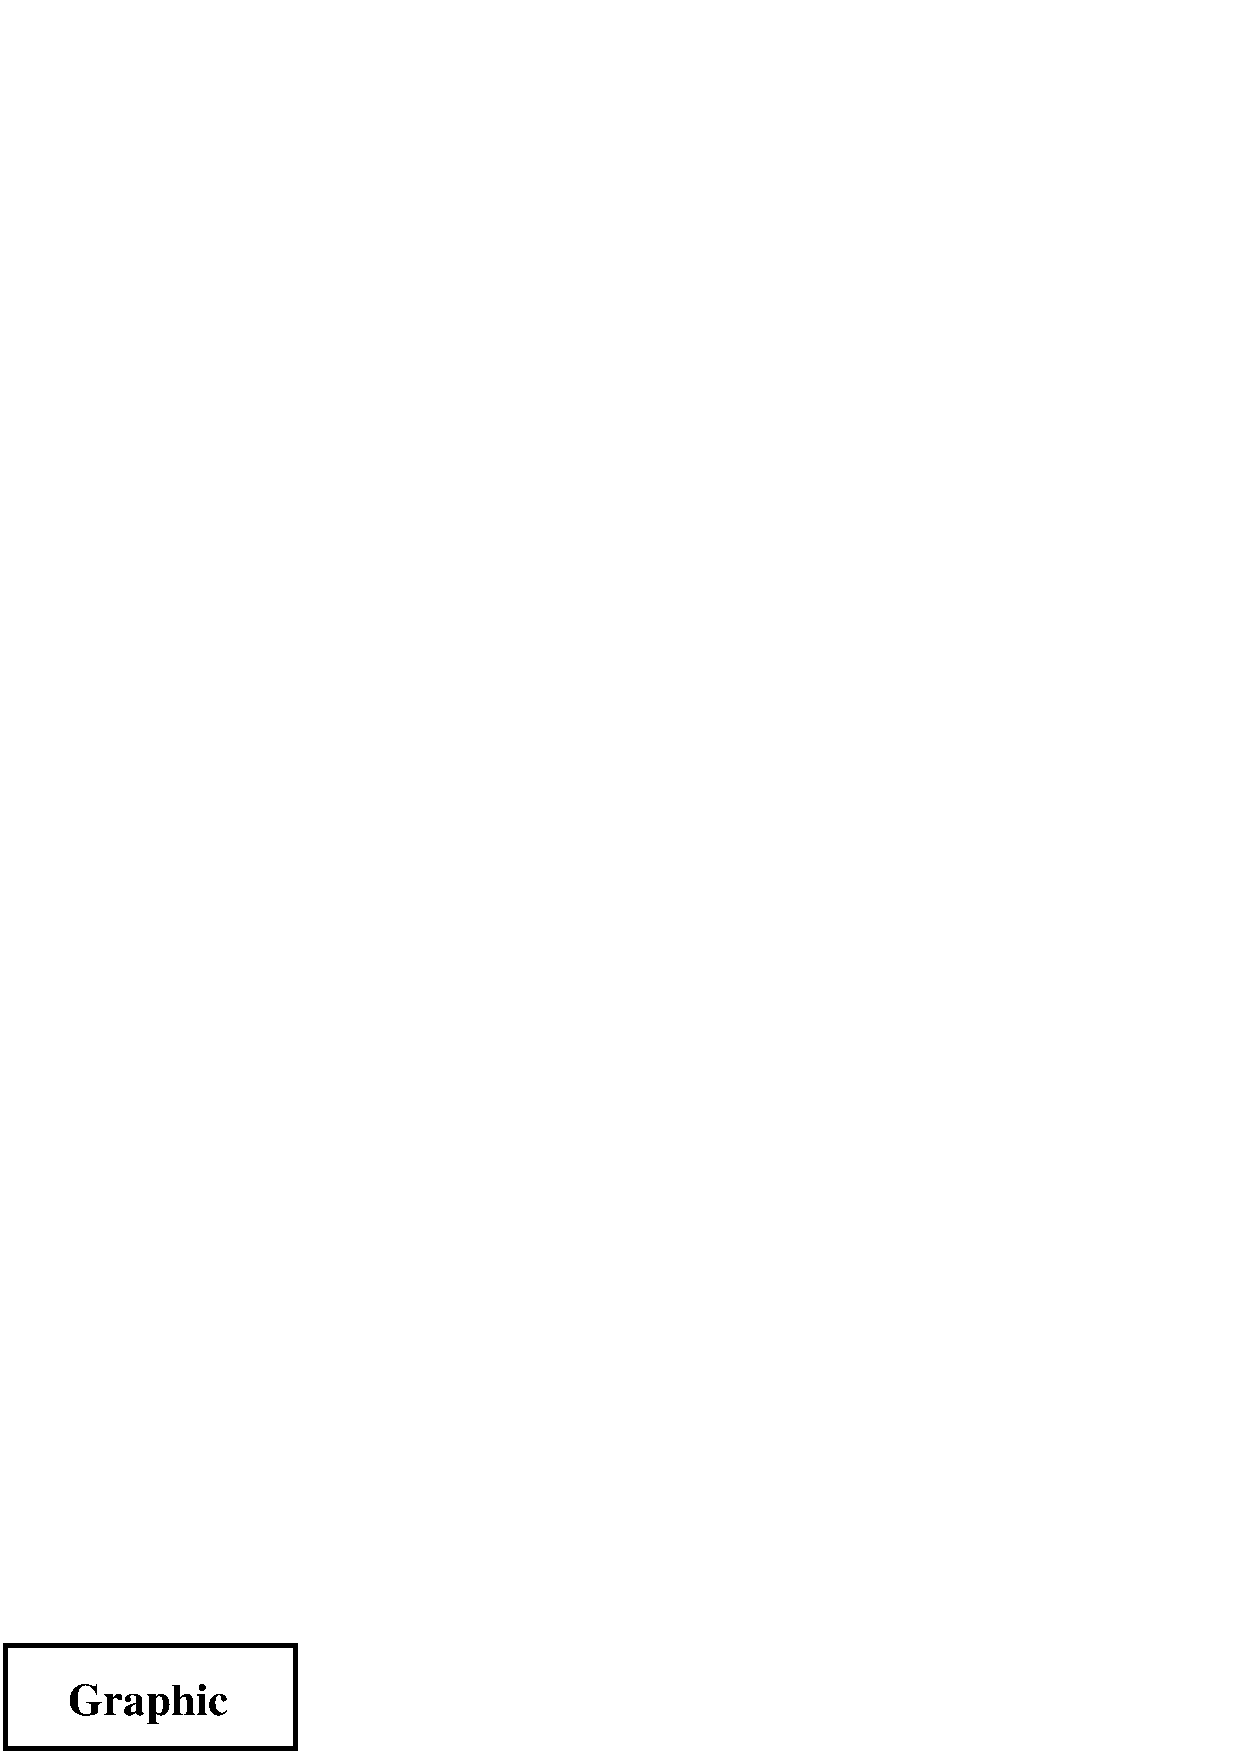
\includegraphics[width=1in]{graphic} 
		\caption{Caption 1}\label{fig:stacked:a}
	\end{minipage}% 
	\hspace{0.04\textwidth}% 
	\begin{minipage}[b]{0.3\textwidth} 
		\centering 
		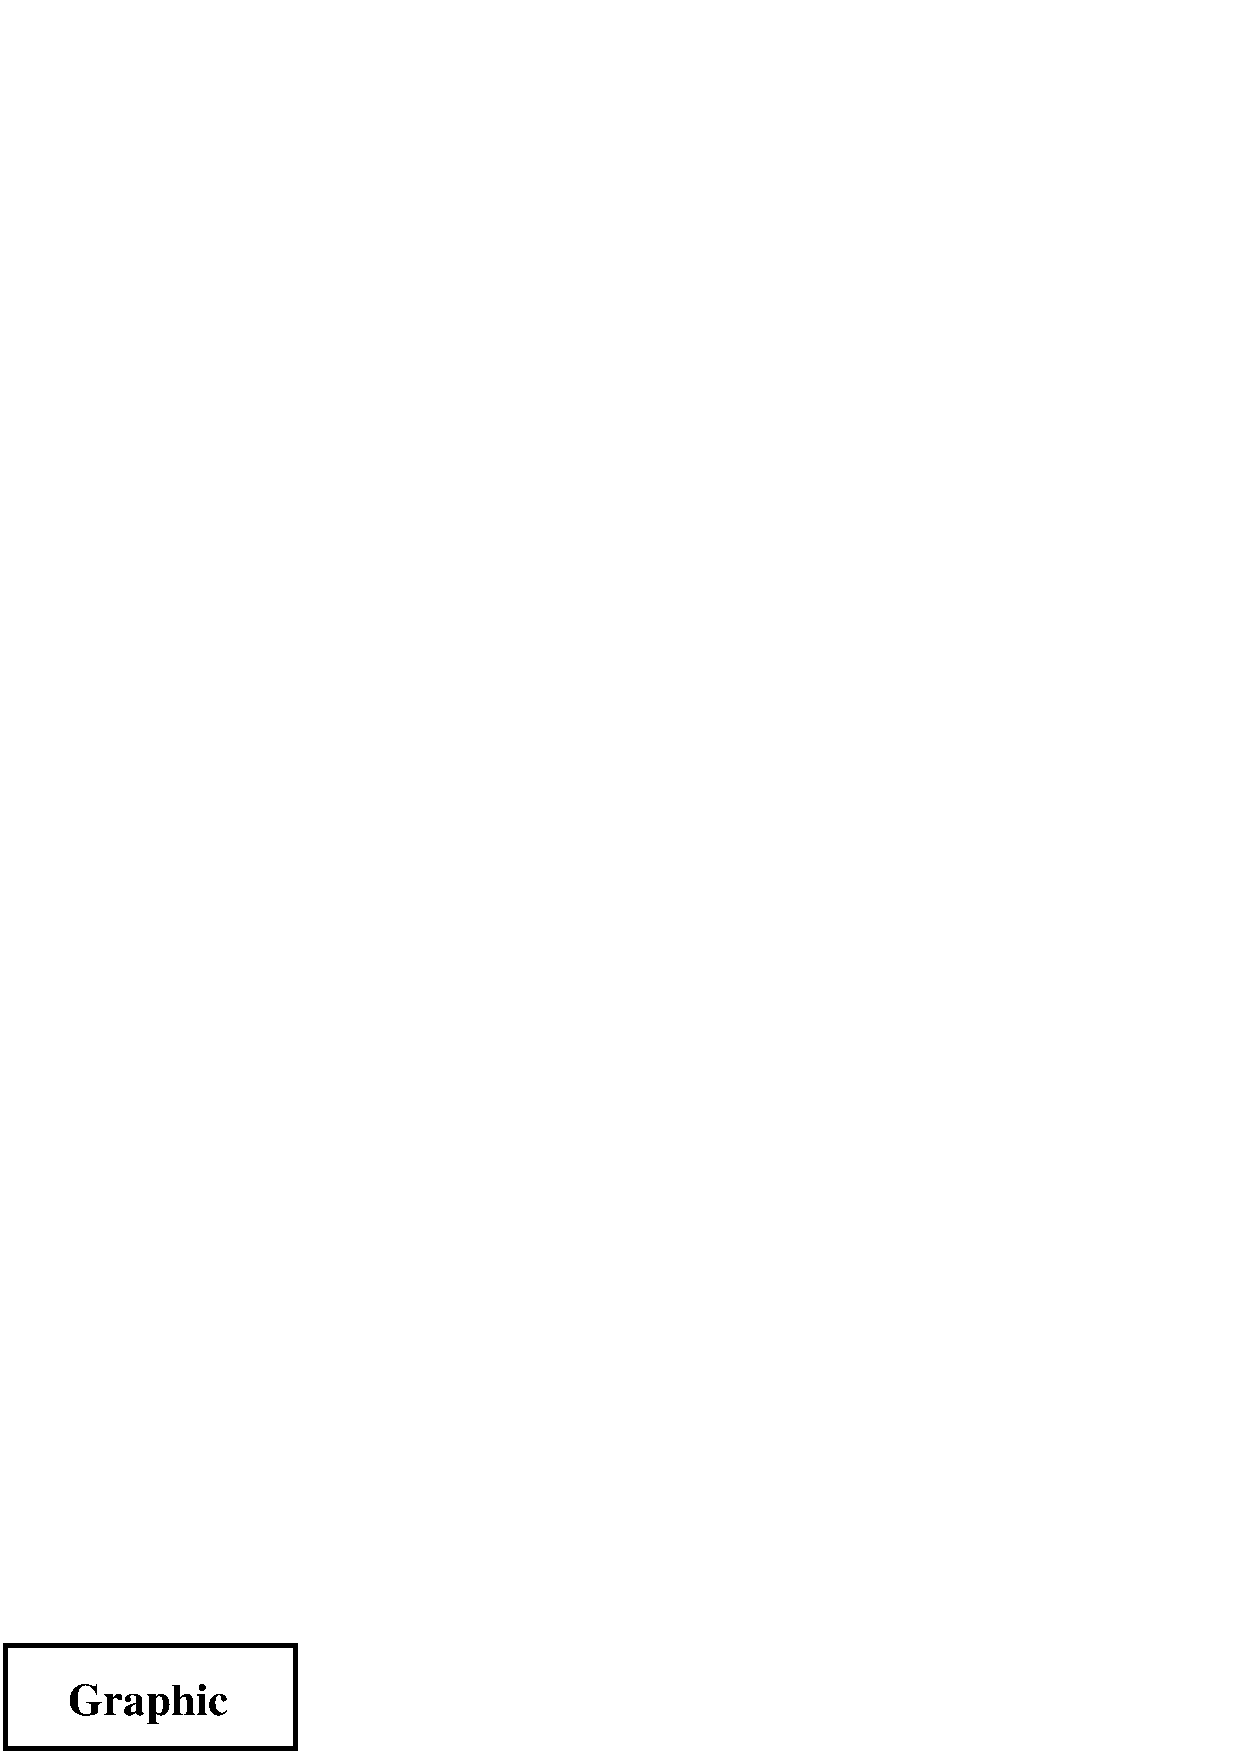
\includegraphics[width=1in]{graphic} 
		\caption{Caption 2} \label{fig:stacked:b}
	\end{minipage}\\[20pt] 
	\begin{minipage}[b]{0.3\textwidth} 
		\centering 
		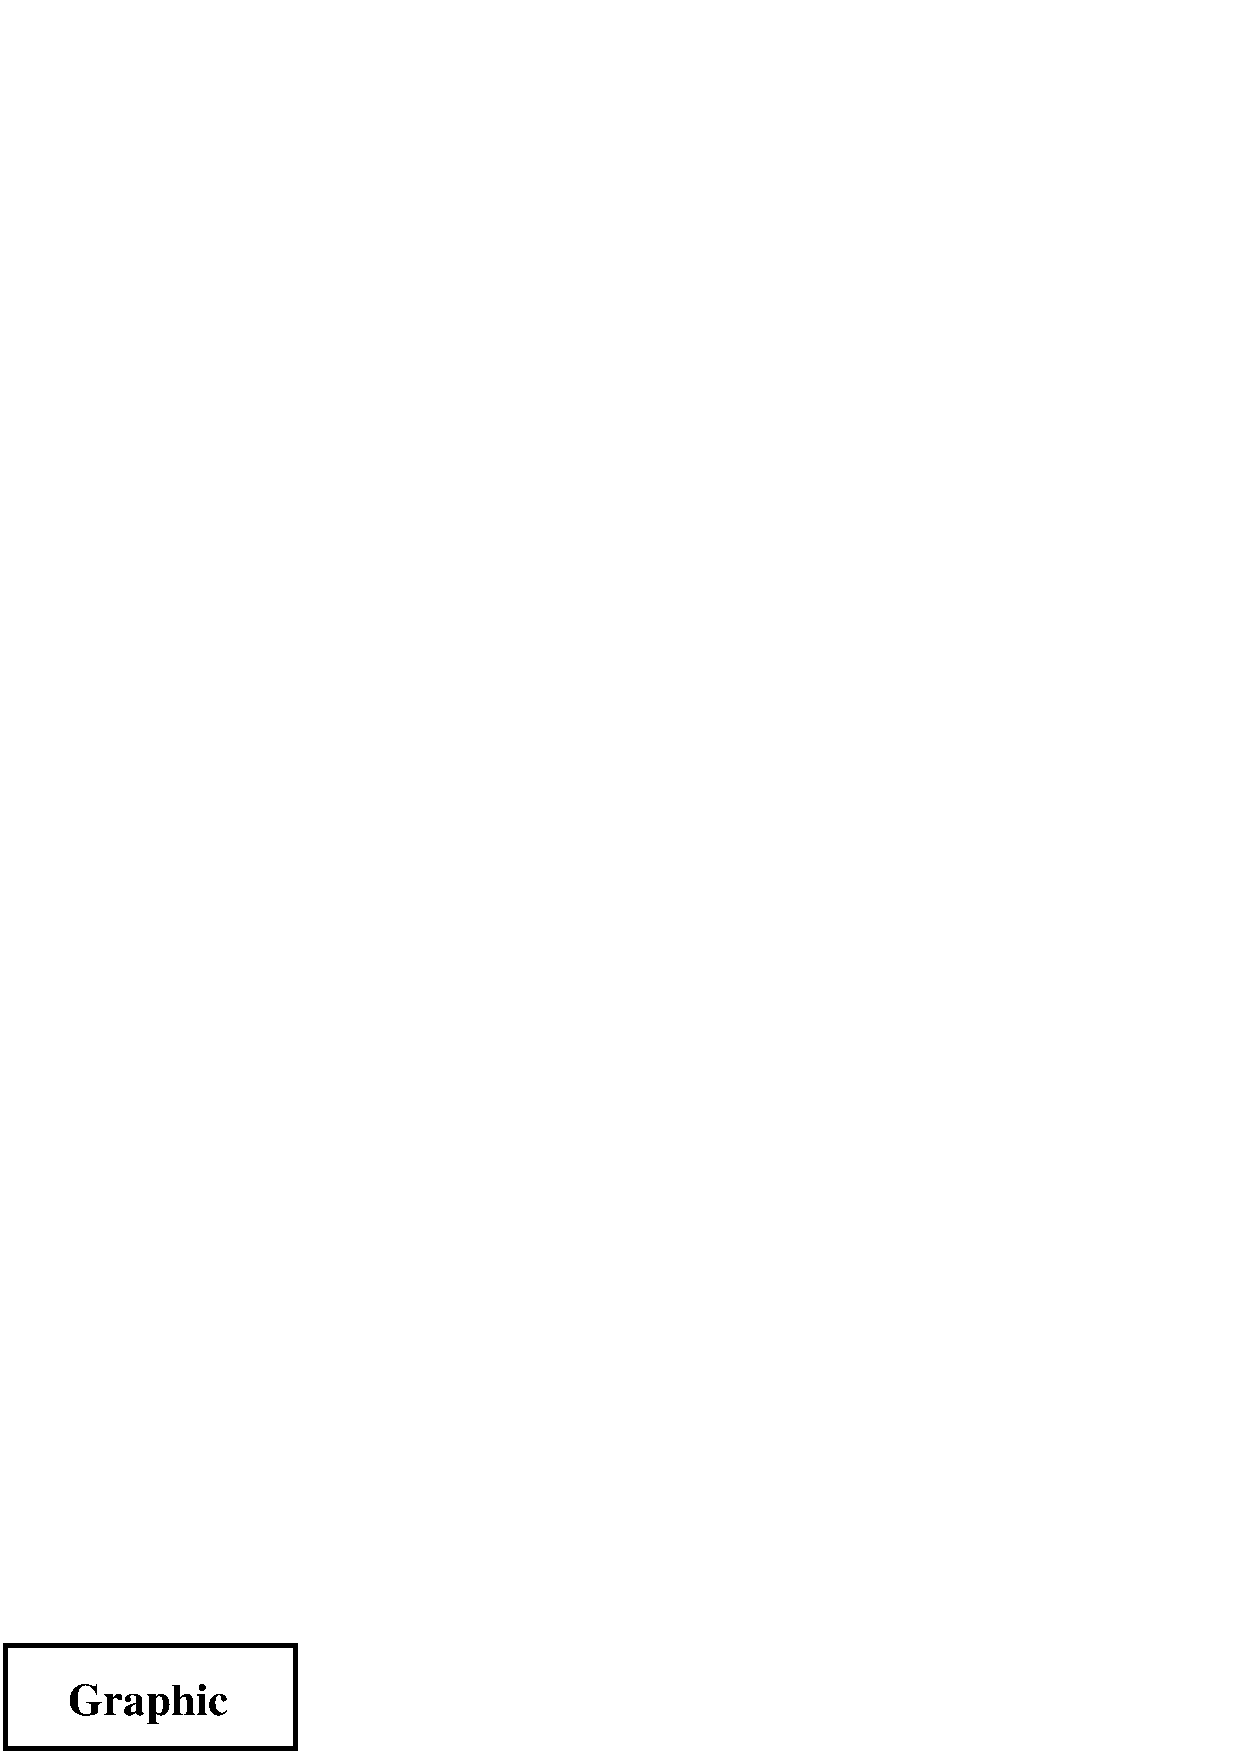
\includegraphics[width=1in]{graphic} 
		\caption{Caption 3} \label{fig:stacked:c}
	\end{minipage}% 
	\hspace{0.04\linewidth}% 
	\begin{minipage}[b]{0.3\textwidth} 
		\centering 
		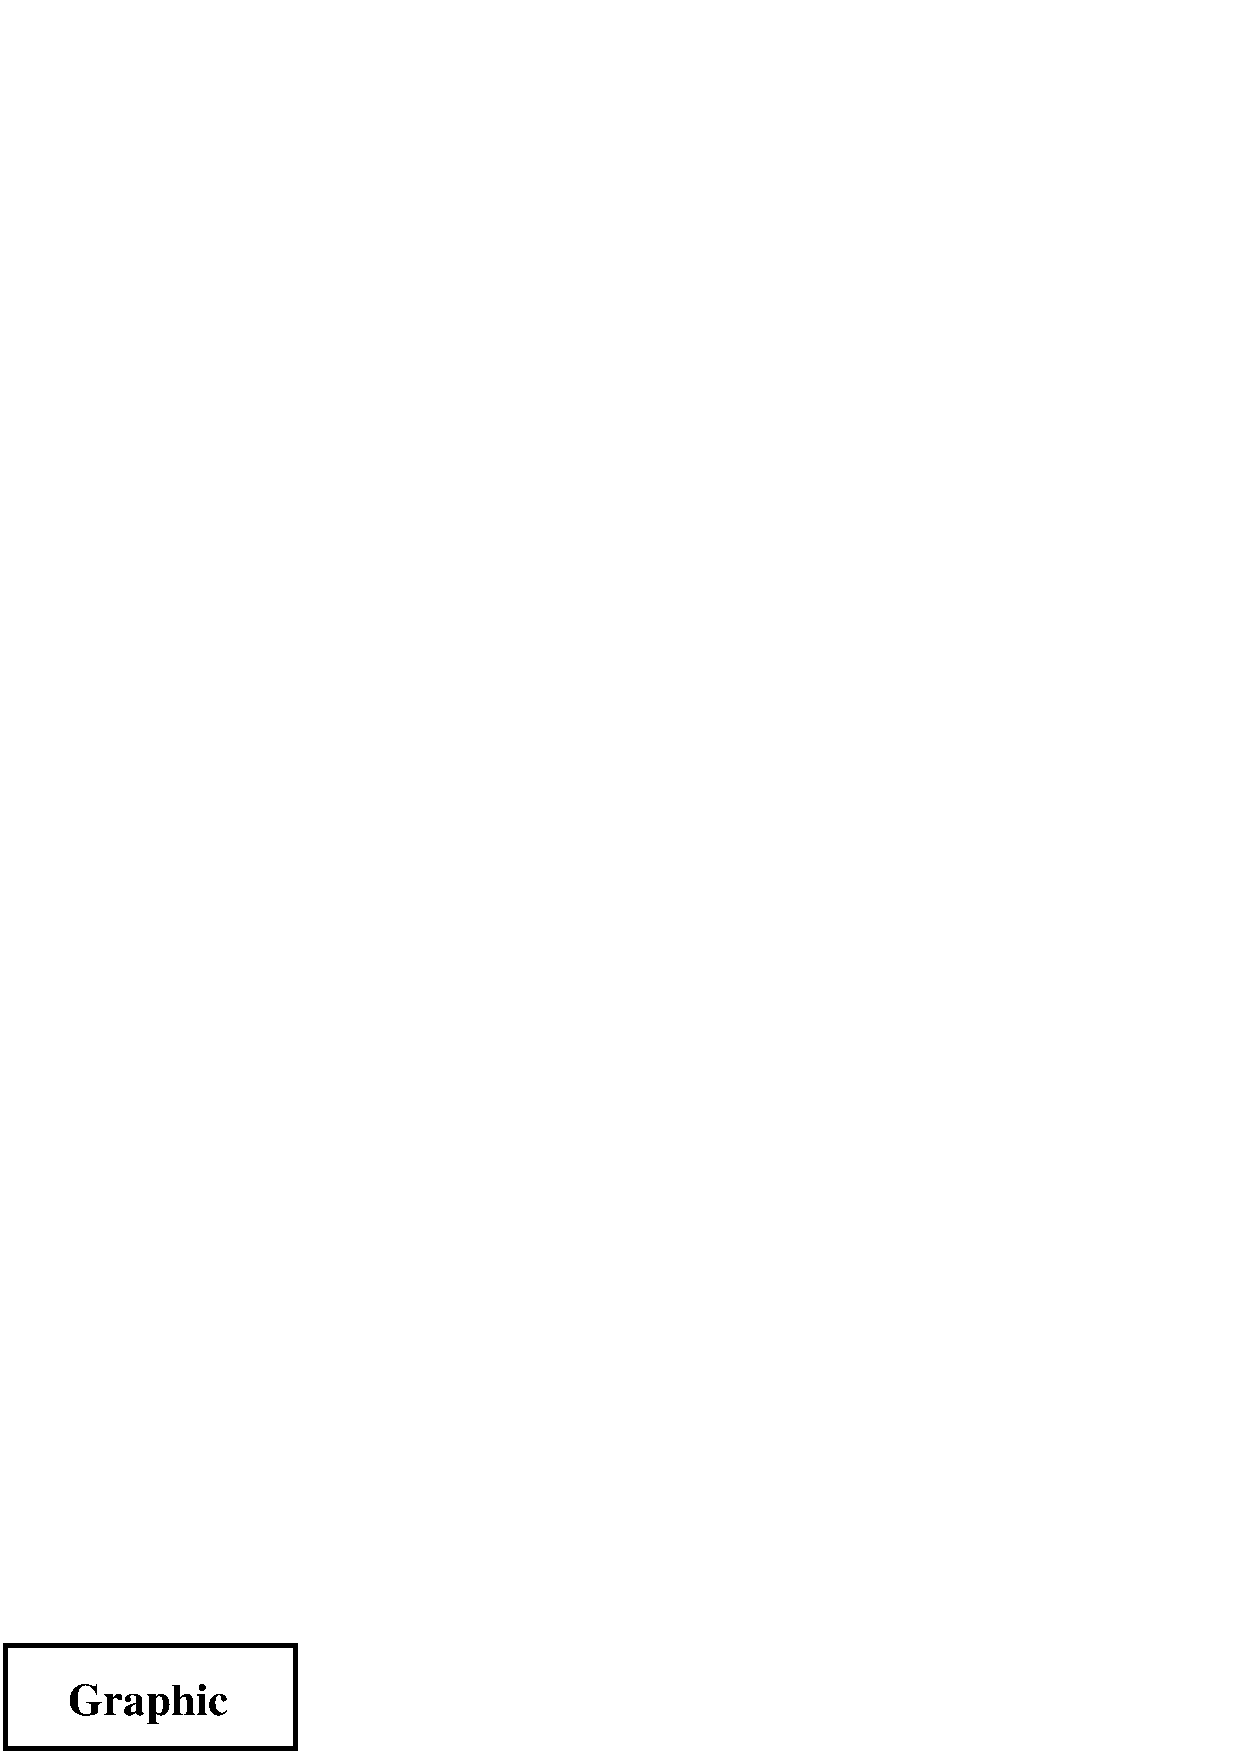
\includegraphics[width=1in]{graphic} 
		\caption{Caption 4} \label{fig:stacked:d}
	\end{minipage}% 
	\hspace{0.04\linewidth}% 
	\begin{minipage}[b]{0.3\textwidth} 
		\centering 
		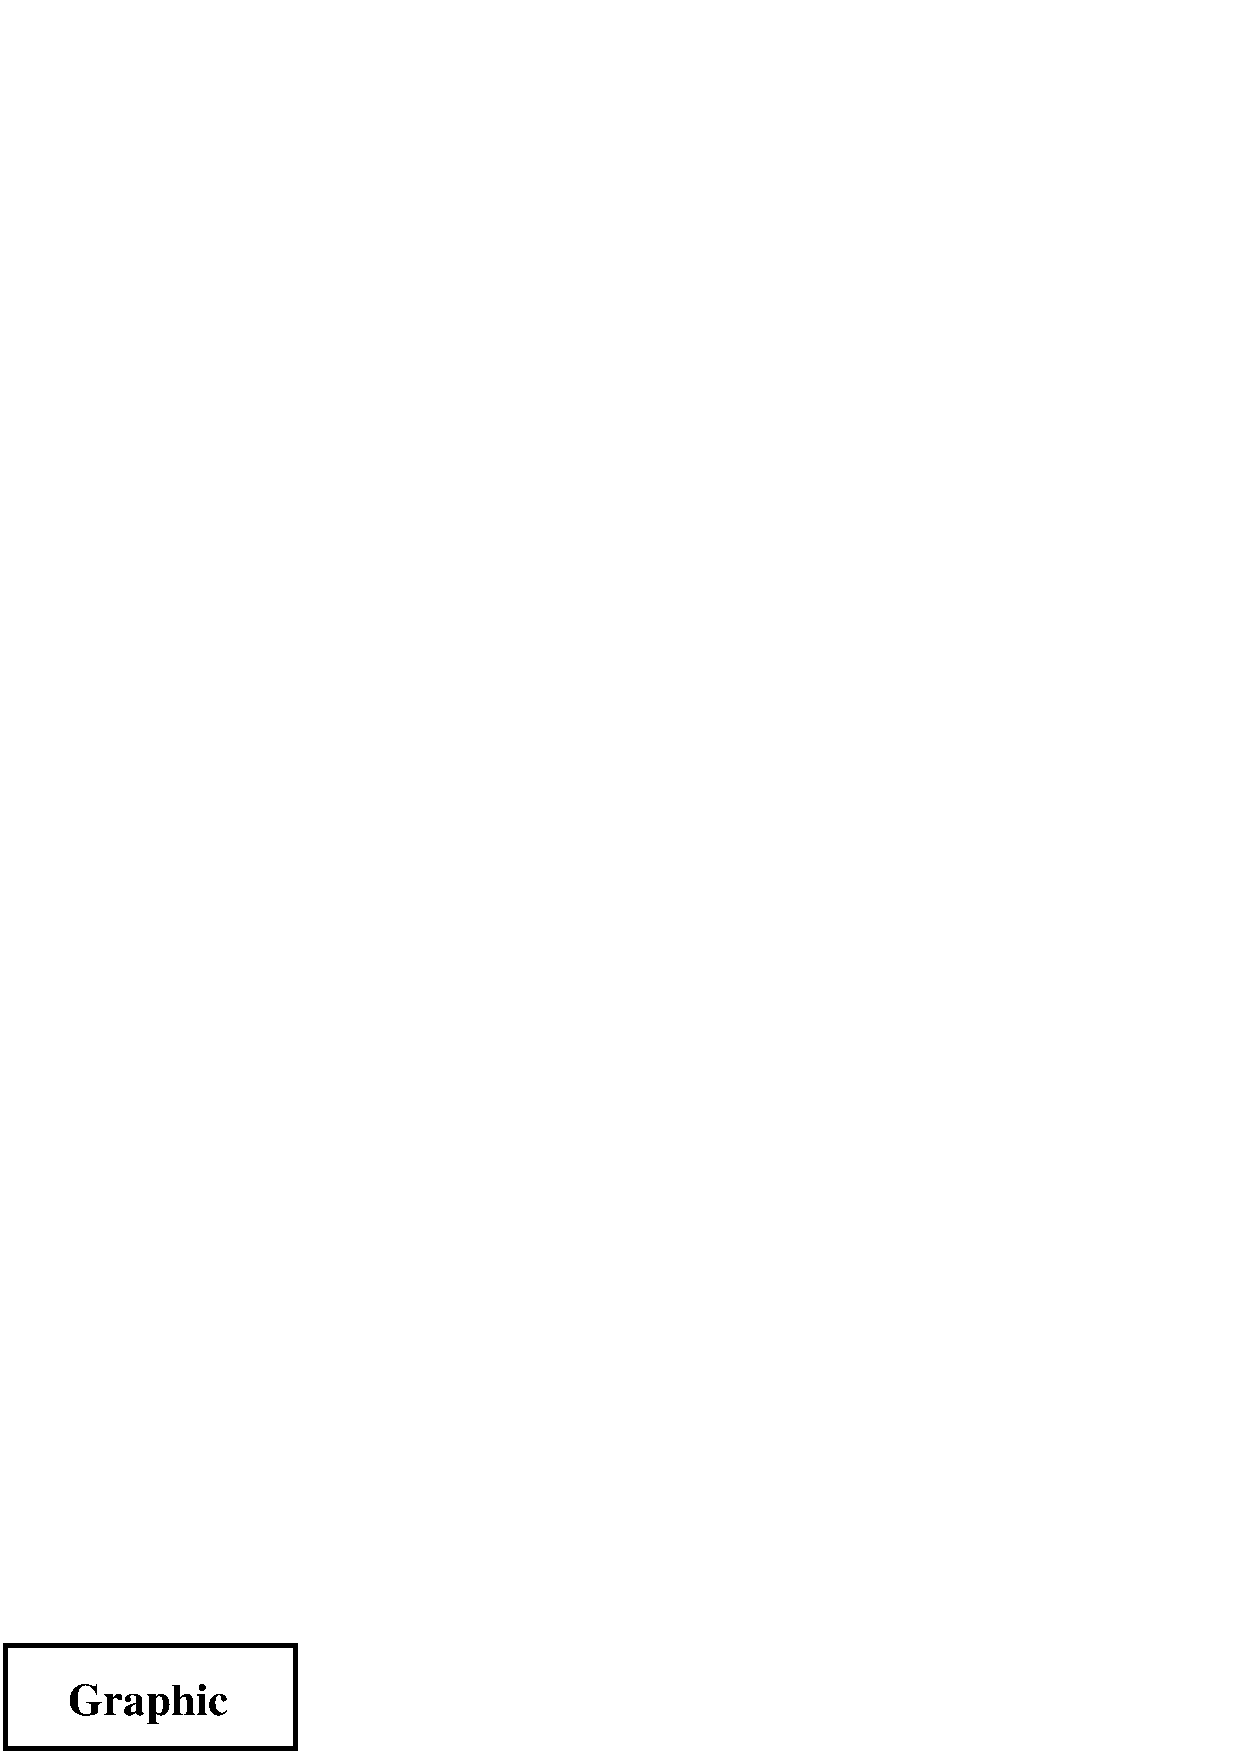
\includegraphics[width=1in]{graphic} 
		\caption{Caption 5} \label{fig:stacked:e}
	\end{minipage} 
\end{figure}

\section{The subfig package}

\section{连续图形}

当两个相邻的图形含有关系较为密切的材料时,常常希望具有相同的
图形编号。因为计数器~\texttt{figure}~中记录了下一图形的编号,
所以可在图形环境前减低~\texttt{figure}~的值使得两幅图形具有
相同的编号。例如:
\begin{Verbatim}[xleftmargin=1cm]
\addtocounter{figure}{-1} 
\begin{figure}
\end{Verbatim}
不过,这样做会使得两幅图形无法被正确区分,导致~\LaTeX{}~的引用
等的混乱。

构造连续图形的最好的方法是使用~\textsf{subfigure}~宏包。
这样既可以使连续的几幅图形具有相同的编号,如~``{\CJKfamily{hei}图}~12'',
且其中的每幅图形也有自己的标记,如~``{\CJKfamily{hei}图}~12(a)''~等。
由于连续的子图位于不同的~\texttt{figure}~环境,所以在两个图形环境
之间,必须减低计数器~\texttt{figure}~的值。
\begin{Verbatim}[xleftmargin=1cm]
\addtocounter{figure}{-1} 
\end{Verbatim}
同时,必须在第二幅子图前将子图的计数器~\texttt{subfigure}~加一。
\begin{Verbatim}[xleftmargin=1cm]
\addtocounter{subfigure}{1}
\end{Verbatim}
例如下面的命令得到两个连续的子图。
\begin{Verbatim}[xleftmargin=1cm]
\begin{figure} 
\centering 
\subfigure[First Part]{% 
\label{fig:graphics:a}% label for subfigure 
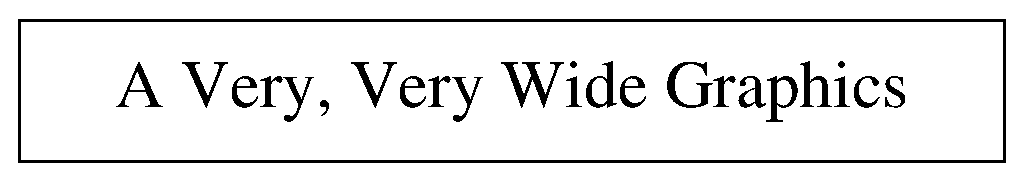
\includegraphics[width=\textwidth]{wide.eps}}% 
\caption{Large Graphics}% 
\label{fig:graphics}% label for figure
\end{figure} 
\addtocounter{figure}{-1} 
\begin{figure} 
\addtocounter{subfigure}{1} 
\centering 
\subfigure[Second Part]{% 
\label{fig:graphics:b}% label for subfigure 
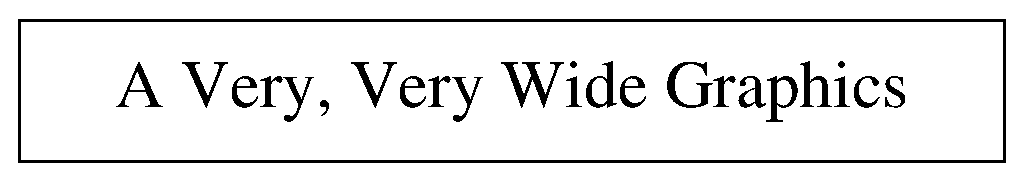
\includegraphics[width=\textwidth]{wide.eps}}% 
\caption{Large Graphics (con't)}% 
\end{figure}
\end{Verbatim}

\begin{figure} 
	\centering 
	\subfigure[First Part]{% 
		\label{fig:graphics:a}% label for subfigure 
		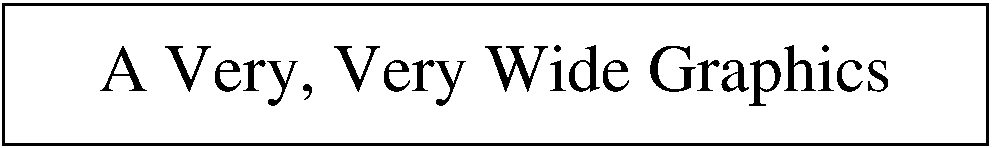
\includegraphics[width=\textwidth]{wide}}% 
	\caption{Large Graphics}%   
	\label{fig:graphics}% label for figure
\end{figure} 
\addtocounter{figure}{-1} 
\begin{figure} 
	\addtocounter{subfigure}{1} 
	\centering 
	\subfigure[Second Part]{% 
		\label{fig:graphics:b}% label for subfigure 
		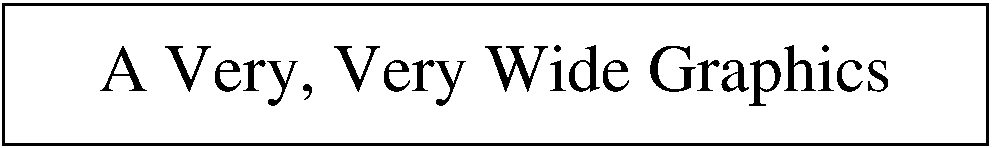
\includegraphics[width=\textwidth]{wide}}% 
	\caption{Large Graphics (con't)}% 
\end{figure}

在这一例子中,每个图形环境中只有一个子图。而当像第~\ref{sec:sidesubfigure}~
节中那样每个图形环境中有多个子图,就需要根据第一个图形环境中子图的个数来
相应地调整计数器~\texttt{subfigure}~的增加值。另外,由于连续图形都是不
同的浮动对像,有可能不出现在连续的页面上。如果出现这种情况,可在最后
一幅连续图形后使用命令~\cmd{FloatBarrier}~来迫使~\LaTeX{}~将连续图形
放置在一起。


\endinput
